\documentclass[a4paper, twoside, 11pt, openright]{article}
\usepackage[utf8]{inputenc}
\usepackage{polski}
\usepackage{float}
\usepackage[T1]{fontenc}

\usepackage{url}
\usepackage{longtable}
\usepackage{a4wide}
\raggedbottom
\usepackage{tabularx, booktabs}

\usepackage[left=3.0cm, right=2.0cm, top=2.5cm, bottom=2.5cm]{geometry}


% PERSONAL data about the thesis
\newcommand{\myTitle}{Metodyka porównania algorytmów prognozy do wspomagania decyzji giełdowych}
\newcommand{\myName}{Nikodem Wiśniewski}
\newcommand{\myNumber}{260907}
\newcommand{\myThesisType}{Praca dyplomowa magisterska}
\newcommand{\myCourse}{Informatyka}
\newcommand{\myProf}{dr hab. inż. Jerzy Balicki, profesor PW}
\newcommand{\myFaculty}{Wydział Matematyki i Nauk Informacyjnych}
\newcommand{\myUni}{Politechnika Warszawska}
\newcommand{\myLocation}{Warszawa}
\newcommand{\myYear}{2019}
\newcommand{\myKeywords}{}
\newcommand{\myKeywordsPL}{}



% DOCUMENT settings


\usepackage{graphicx}
\usepackage{multirow}
\usepackage{indentfirst}
\usepackage{wrapfig}
\usepackage[font=footnotesize, % equivalent to 9 pt font
			labelfont=bf, 
			justification=justified, 
			singlelinecheck=false]{caption} 
%\usepackage[justification=centering]{subcaption} % two images side by side captions
\usepackage{tabularx, booktabs} % pretty LaTeX tables
\usepackage{siunitx} % units SI e.g. \SI{10}{\kilogram\per\meter\square}
\usepackage{mathtools} % amsmath, symbols such as brackets, arrows, equation numbering only for referrenced eqs.
%\usepackage[parfill]{parskip} % spacing between paragraphs instead of indent
%\parfillskip 0pt plus 0.75\textwidth % get rid of widows at the end of paragraphs
\frenchspacing % for "Polish" spaces after the sentence
\usepackage{polski} % Polish rules of hyphenation
\usepackage{dashrule} % for dotted lines in declarations page
\usepackage{emptypage} % removes headers on empty pages
\usepackage{fancyhdr} % header and footer settings
\usepackage{subfigure}
\usepackage{cleveref}


\pagestyle{fancy}
\fancyhf{}
\newcommand{\fncyfront}{%
	\fancyhead[RO]{}
	\fancyfoot[RO]{}
	\fancyhead[LE]{}
	\fancyfoot[LE]{}
	\fancyhead[RE,LO]{}
	\fancyfoot[C]{}
	\renewcommand{\headrulewidth}{0pt}}
\newcommand{\fncymain}{%
	\fancyhead[RO]{{\footnotesize \rightmark}}
	\fancyfoot[RO]{\thepage}
	\fancyhead[LE]{{\footnotesize \leftmark}}
	\fancyfoot[LE]{\thepage}
	\fancyfoot[C]{}
	\renewcommand{\headrulewidth}{0.3pt}}
	
\renewcommand*{\tablename}{Tabela} 
	
\newcolumntype{P}[1]{>{\centering\arraybackslash}p{#1}}
\newcolumntype{M}[1]{>{\centering\arraybackslash}m{#1}}



% FONT settings
\usepackage[T1]{fontenc}

%\renewcommand{\familydefault}{\sfdefault} % change font to sans serif
\usepackage{amsfonts} % mathematical fonts
\usepackage{inconsolata} % monospaced font in urls and \texttt
%\usepackage{url}
%\urlstyle{same}

% DEBUG
\usepackage{lipsum}
\usepackage{etoolbox} % removes page number in table of contents
\patchcmd{\chapter}{plain}{empty}{}{}


\begin{document}
\fncyfront
%*******************************************************
% Titlepage
%*******************************************************
\begin{titlepage}
\begingroup
\begin{center}		
			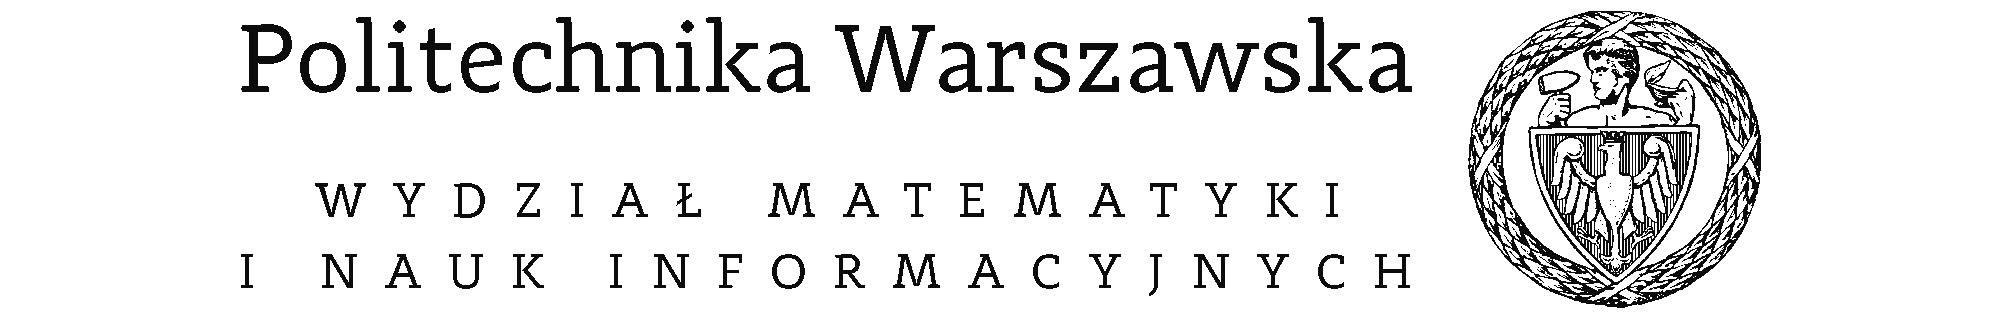
\includegraphics[width=1.0\textwidth]{img/pw_header}
			
			\vspace{1.0cm}
			\fontsize{24}{30}\selectfont\myThesisType
			\fontsize{12}{14}\selectfont
			
			\vspace{0.5cm}
			na kierunku \myCourse \\
			\vspace{1cm}
			{\fontsize{14}{18}\selectfont \myTitle} \\ 
			
			\vspace{1.5cm}
			\fontsize{21}{25}\selectfont \myName \\
			\fontsize{12}{14}\selectfont
			Numer albumu \myNumber \\

			\vspace{6.5cm}
			promotor \\
			\myProf \\
			\vspace{0.5cm}
			\vfill 
			Warszawa, \myYear
        \vfill                      
\end{center}
\endgroup
\end{titlepage}

\cleardoublepage

\begingroup
\fontsize{12pt}{14.4pt}\selectfont

\begin{abstract}

Giełda jest miejscem przyciągającym rzesze inwestorów pragnących pomnożyć swój kapitał. Właściwy handel instrumentami finansowymi na giełdzie pozwala na osiąganie zysków przekraczających zyski z alternatywnych inwestycji takich jak na przykład nieruchomości. Skuteczna inwestycja na giełdzie zazwyczaj opiera się o wybór odpowiednich spółek. Przy aktywnym zarządzaniu portfelem akcji podejmowane decyzje o sprzedaży i kupnie są ważniejsze od doboru spółek. Wiąże się to oczywiście z dużym ryzykiem i wymaga wiedzy z dziedziny ekonomii. Co jeżeli udałoby się opracować model decyzyjny, umożliwiający grę na giełdzie  bez wiedzy eksperckiej? 

\bigskip

Celem niniejszej pracy było stworzenie algorytmu decyzyjnego, który umożliwi skuteczne zarządzanie portfelem inwestycyjnym dowolnej osobie. W pracy opisano charakterystykę giełdy, dostępne dane giełdowe oraz różne podejścia do tematu przewidywania cen na giełdzie. Ponadto podjęto próbę stworzenia algorytmów do prognozowania za pomocą modeli z dziedziny uczenia maszynowego. Zostały wykorzystane takie modele jak: sztuczne sieci neuronowe, maszyny wektorów nośnych, lasy losowe czy też metoda \textit{Light GBM}. Do oceny i porównywania jakości modeli została wykorzystana miara dokładności oraz miara \textit{AUC}. Następnie, w celu dalszej oceny skuteczności, została wykonana symulacja zautomatyzowanego handlu na giełdzie za pomocą prostego algorytmu decyzyjnego wykorzystującego stworzone modele. 


\bigskip

	\noindent \textbf{Słowa kluczowe:} giełda, predykcja, klasyfikacja, sieci neuronowe, SVM, las losowy, Light GBM, uczenie maszynowe, wspomaganie decyzji giełdowych
\end{abstract}

\newpage


\renewcommand{\abstractname}{Abstract}
\begin{abstract}

Thesis title: \textbf{Comparision methodology of some prediction algorithms for stock market decision making}

\bigskip

The stock market is attracting many inverstors willing to earn money. Trading with securities in the right way can outmatch profits made in alternative investments such as real estate. An effective stock market investment usually relies on choosing the proper companies. When actively managing one's investment portfolio (e.g. day trading) accurate decisions about buying and selling securities are far more critical than the company choice. Active trading carries a lot of risk and requires plenty of economical domain knowledge. What if a decision model could be designed, facilitating active investing without expertise?

\bigskip

The goal of this dissertation is to create a decision algorithm, enabling effective investmen portfolio managment for anyone. This work describes stock market features, available data and various approaches to stock price prediction. Moreover this paper attempted creating a prediction algorithm using machine learning techniques. Models such as artificial neural networks, SVM, random forests or \textit{Light GBM} were employed. Model performance was compared using accuracy and the \textit{AUC} metric. Afterwards in order to further analyze model quality a stock market automatic trading simulation was carried out. In this simulation trading was made using above models wrapped with a simple decision algorithm.

	
	\bigskip
	
	
	\noindent \textbf{Keywords:} stock market, predicting, classification, neural networks, SVM, random forest, Light GBM, machine learning, supporting stock market decisions
\end{abstract}

\cleardoublepage


\hfill
\begin{table}[b]
\centering
\begin{tabular}[t]{ccc}
............................................. & \hspace*{100pt} & .............................................\\
podpis promotora & \hspace*{100pt} & podpis autora
\end{tabular}
\end{table}

\fncymain



\cleardoublepage

\tableofcontents

\cleardoublepage

\section{Wprowadzenie}

Giełda z definicji jest miejscem wymiany towarów przez sprzedawców i kupców. Giełdy można podzielić na giełdy towarowe, pieniężne lub usługowe. Wymiany na tradycyjnych giełdach przebiegają przede wszystkim podczas sesji, które są organizowane w określonych dniach i godzinach. Najpopularniejszym rodzajem giełd są giełdy pieniężne, a w szczególności giełdy papierów wartościowych. Największymi giełdami papierów wartościowych są \textit{NYSE (New York Stock Exchange)}\cite{nyse}, \textit{Nasdaq}\cite{nasdaq} oraz \textit{JPX (Japan Exchange Group)}\cite{jpx}. Na każdej z tych giełd w dniach, w których prowadzone są sesje, dochodzi do transakcji opiewających na łączną kwotę rzędu miliardów dolarów amerykańskich.

\bigskip

 Jednym z wymienianych na giełdzie towarów są akcje różnorodnych spółek. Każda spółka, która jest obecna na giełdzie ma przypisany do siebie symbol giełdowy (\textit{ticker}). Symbol giełdowy jest skrótowym kodem do identyfikowania spółek na określonej giełdzie (przykładowe symbole: \textit{GOOGL}, \textit{MSFT}, \textit{AMZN}). Podczas każdej sesji dokonywane są transakcje milionów akcji, których cena regulowana jest przez wolny rynek. Wynikiem tego jest duża zmienność cen i nieprzewidywalność akcji. Jest ona spowodowana między innymi: spekulacjami inwestorów, upublicznianiem informacji o konkretnej spółce (np. raportów finansowych) lub wydarzeniami na arenie politycznej (np. ustawy wpływające na działalność spólek z konkretnego sektora). Poprawne przewidywanie zmian cen giełdowych oznacza dla inwestora możliwość wypracowania zysków na kupnie i sprzedaży akcji.
 
\bigskip

Temat predykcji i spekulacji giełdowych był wielokrotnie poruszany w prasie naukowej. Wielu naukowców pracowało nad predykcją dokładnej wartość ceny akcji na przykład za pomocą sieci radialnych (Guo \& Wang \& Yang \& Miller, 2015 \cite{paper_regression_radial}). Często można spotkać prace traktujące o problemie wyznaczania trendu ceny, a więc problemu klasyfikacji. Klasyfikacja trendu giełdowego za pomocą maszyn wektorów nośnych została opisana między innymi przez \textit{Kim} (2003) \cite{paper_classification_svm}. Większość prac skupia się jednak na na predykcji trendu indeksów, aniżeli konkretnych spółek (Kara \& Boyacioglu \& Baykan, 2011 \cite{paper_classification_index_istanbul}; Patel \& Shah \& Thakkar \& Kotecha, 2015 \cite{paper_classification_index_sp500}). Według najlepszej wiedzy autora tej pracy, brak jest źródeł naukowych opisujących predykcje dla konkretnych spółek giełdowych, wraz z wykorzystaniem przewidywanych wartości do wspomagania decyzji giełdowych. 

\newpage

\section{Modele prognozy na giełdzie oraz kryteria ich oceny}

Poniżej opisane zostały dane giełdowe pochodzące z wielu źródeł, zróżnicowane sposoby na predykcje cen na giełdzie oraz różnorodne kryteria oceny modeli predykcyjnych. 

\subsection{Dane giełdowe}

Istnieje wiele rodzajów danych, które są w większym lub mniejszym stopniu powiązane z giełdą papierów wartościowych. Zbiór informacji, które można wykorzystywać w przewidywaniu cen akcji jest bardzo szeroki, począwszy od cech bezpośrednio opisujących akcje na giełdzie, przez dane opisujące finansową sytuację spółek emitujących akcje, wskaźniki będące statystycznym odzwierciedleniem zmian cen na giełdzie, aż po dane alternatywne takie jak sentyment powiązany z wiadomościami na temat spółek oraz giełdy.

\subsubsection{Dane podstawowe}

Podstawowymi (dziennymi) danymi wynikającymi bezpośrednio z funkcjonowania giełdy są:

\begin{itemize}
\item{Data}
\item{Cena zamknięcia} - cena akcji pod koniec dnia
\item{Cena otwarcia} - cena akcji na początku dnia
\item{Liczba akcji w obrocie danego dnia}
\item{Najniższa cena akcji danego dnia}
\item{Najwyższa cena akcji danego dnia}
\end{itemize}

 Przy korzystaniu z wartości cen akcji należy również uwzględnić podział akcji(tak zwany \textit{split}). Gdy jakaś spółka decyduje się na podział swoich akcji oznacza to, że każda z akcji dzieli się na dwie akcje o cenie wynoszącej połowę pierwotnej ceny. Taki zabieg pozwala na zmniejszenie ceny pojedynczej akcji dzięki czemu może stać się ona dostępna dla większej liczby inwestorów. 
 
\bigskip

Powyższe dane nie wnoszą jednak zbyt wiele informacji ponieważ są odzwierciedleniem powstałego obrotu akcji na giełdzie, a nie jego przyczyną. W związku z dużą losowością ruchów giełdowych, są niewystarczające aby skutecznie przewidzieć zmiany cen akcji. Zawodowi maklerzy do podejmowania swoich decyzji wspomagają się dodatkowo dwoma technikami: \textbf{analizą fundamentalną} oraz \textbf{analizą techniczną}.

\subsubsection{Analiza fundamentalna}

Analiza fundamentalna \cite{fundamentalanalysis} spółek jest analizą kondycji ekonomicznej spółek w zestawieniu z wartością ich akcji. Ten rodzaj analizy ma odpowiedzieć na pytanie czy cena akcji konkretnej spółki odpowiada jej sytuacji na rynku. Przy takim badaniu spółki brane jest pod uwagę wiele różnych czynników, takich jak:
\begin{itemize}
\item{analiza finansowa spółki}
\item{analiza sektorowa}
\item{analiza makroekonomiczna}
\item{analiza ogólnej sytuacji spółki}
\end{itemize}

Ten rodzaj badania spółek jest niezwykle czasochłonny i często wymaga eksperckiej wiedzy w dziedzinie finansów. Dodatkowo analiza fundamentalna wymaga posiadania danych, publicznych aczkolwiek czasami ciężko dostępnych, o spółkach i sektorach, w których się znajdują. Analizę fundamentalną stosuje się w szczególności przy inwestycjach długoterminowych (np. kilka miesięcy).

Najsłynniejszym analitykiem technicznym świata jest \textit{Warren Buffet} prezes amerykańskiego holdingu \textit{Berkshire Hathaway \cite{berkeshire}}. 

\subsubsection{Analiza techniczna}

Analiza techniczna \cite{technicalanalysis} jest zbiorem technik mających na celu wspomaganie inwestora w podejmowaniu decyzji na podstawie historycznych danych giełdowych. Analiza ta bada zachowania rynku oraz poszukuje trendów np. poprzez analizę kształtów wykresów giełdowych. Szczególnie istotne są liczne wskaźniki techniczne oraz narzędzia analizy statystycznej.

Najpopularniejsze wskaźniki techniczne obejmują:
\begin{itemize}
\item{\textbf{SMA} (ang. Simple Moving Average)} - średnia krocząca. Jest to średnia cen z kilku ostatnich dni (np. 3, 7, 14, 30),
\item{\textbf{EMA} (ang. Exponential Moving Average)} - wykładnicza średnia krocząca. Jest to wykładnicza średnia cen z kilku ostatnich dni (np. 3, 7, 14, 30),
\item{\textbf{MACD} (ang. Moving Average Convergence Divergence)} -  miara zbieżności i rozbieżności średnich ruchomych,
\item{\textbf{RSI} (ang. Relative Strength Index)} -  wskaźnik siły względnej określający siłę trendu,
\item{\textbf{oscylator stochastyczny}} -  wskaźnik momentum i siły trendu.
\end{itemize}

\subsubsection{Źródło danych}

W pracy zostało wykorzystane darmowe źródło danych giełdowych \textit{Alpha Vantage} \cite{alphavantage}. Jest to API (ang. Application Programming Interface) pozwalające na pobranie historycznych danych giełdowych dla konkretnej spółki poprzez podanie odpowiedniego symbolu giełdowego. Dostępne są zarówno podstawowe dane giełdowe jak i wskaźniki analizy technicznej. 

\bigskip

Na giełdach papierów wartościowych są obecne tysiące spółek. Ze względu na ograniczone zasoby obliczeniowe oraz dostępność danych badania zostały przeprowadzone na spółkach z giełdy \textit{NASDAQ} o największej kapitalizacji.

\subsection{Predykcja}

Na rysunku \ref{img:alphabet_history} widoczne są zmiany cen akcji spółki \textit{Alphabet Inc.} w latach 2004-2018. Analizując ten wykres z łatwością można wskazać daty, w których opłacalnym było zainwestowanie w akcje, aby następnie je sprzedać w póżniejszym terminie by osiągnąć zysk. Niestety stwierdzenie czy wartość akcji w przyszłości spadnie, czy wzrośnie, nie jest tak trywialne jak odczytywanie danych historycznych. Przewidywanie przyszłych cen akcji jest głównym zajęciem zarówno inwestorów indywidualnych jak i instytucjonalnych. Skuteczne odgadywanie przyszłych wzrostów lub spadków cen pozwoliłoby na osiąganie ponadprzeciętnych zysków i unikanie strat. O trudności tego zadania mogą świadczyć takie teorie jak \textit{hipoteza błądzenia losowego} czy też \textit{hipoteza rynku efektywnego}. Zgodnie z \textit{hipotezą błądzenia losowego} \cite{randwalk}, krótkoterminowo, ceny akcji zmieniają się według nieprzewidywalnych schematów. Zmiany minutowe cen akcji są więc dużo trudniejsze do przewidzenia niż zmiany dobowe. \textit{Hipoteza rynku efektywnego} \cite{efficientmarket} opiera się na założeniu iż ceny obecne na giełdzie całkowicie odwzorowują wszystkie dostępne informacje na rynku. Oznacza to, że próby wyprzedzenia innych inwestorów na podstawie szybkiej reakcji na pojawiające się informacje nie będą skuteczne. Obie te hipotezy mają zarówno swoich zwolenników jak i krytyków.

\begin{figure}[H]
\centering 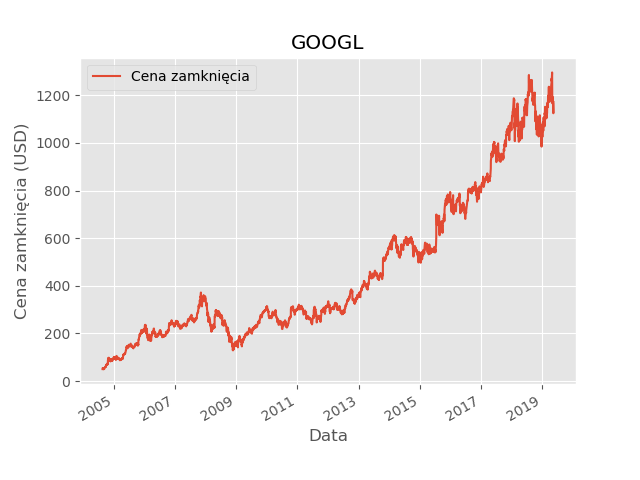
\includegraphics[scale=0.9]{img/GOOGL_adj_close.png}
\caption{Wykres cen akcji spółki \textit{Alphabet Inc} (opracowanie własne)}
\label{img:alphabet_history}
\end{figure}

Rysunek \ref{img:alphabet_history} ilustruje fakt, że ceny zamknięcia akcji tworzą szereg czasowy. Dotyczy to także pozostałych charakterystyk akcji, takich jak cena otwarcia, liczba akcji w obrocie danego dnia, najniższa cena akcji czy najwyższa cena akcji danego dnia. Fakt ten ma istotny wpływ na sposób używania i przetwarzania danych giełdowych.

\subsubsection{Zakres prognozy}

Przed przystąpieniem do konstruowania modeli predykcyjnych należy zdefiniować co tak naprawdę warto przewidywać, każda akcja ma bowiem kilka atrybutów. Najbardziej pożytecznym parametrem akcji, którego wykorzystanie daje inwestorowi największe szanse na zysk jest \textbf{cena zamknięcia}. Znajomość ceny zamknięcia z kolejnego dnia daje inwestorowi cały czas trwania sesji giełdowej na podjęcie skutecznych decyzji inwestycyjnych. Jest to najczęściej wybierany parametr akcji przy przewidywaniu ceny. Przykładem parametru, który nie jest istotny jest liczba akcji w obrocie z kolejnych dni, ta liczba sama w sobie nie niesie informacji o spadku lub wzroście cen.

\bigskip

Po wybraniu celu prognozy należy również określić jej przedział czasowy. Ceny na giełdzie można przewidywać dla dowolnego przedziału czasu. Może to być zarówno okres jednej minuty jak i kilku miesięcy. Przy gwarancji doskonałych prognoz, im większa częstotliwość dokładnego przewidywania ceny tym lepiej. Wynika to z tego iż inwestor może szybciej reagować na zachodzące zmiany i w większym stopniu wykorzystywać pozyskaną wiedzę zwiększając zyski. Z drugiej strony opierając się na \textit{hipotezie błądzenia losowego} można zauważyć, że zmiany w małych przedziałach czasowych są dużo bardziej zaburzone przez losowe wahania ceny. To z kolei sprawia iż krótkoterminowe ruchy cen mogą okazać się nie do przewidzenia. W celu utrzymania kompromisu pomiędzy użytecznością modelu, a jego odpornością na losowość giełdy, za okres predykcji został wybrany \textbf{jeden dzień}.
 
\subsubsection{Prognozowanie - regresja czy klasyfikacja?}

Do tematu prognozowania cen akcji można podejść na dwa sposoby:
\begin{itemize}
\item{\textbf{dokładny}, przewidywanie konkretnych wartości cen akcji,}
\item{\textbf{binarny}, predykcja wzrostu lub spadku ceny - tak zwana predykcja trendu.}
\end{itemize}

Potencjalnie korzystniejszym podejściem jest przewidywanie dokładnych cen akcji, gdyż jest to dokładniejsze aproksymowanie ceny. Jednakże z perspektywy inwestora istotniejszym od dokładnych wartości ceny są trendy. To właśnie różnice w cenach akcji pozwalają zarobić na ich obrocie. Wobec tego zamiast przewidywania dokładnej ceny zamknięcia warto przewidywać wzrosty oraz spadki cen. W przeciwieństwie do danych ciągłych, wyjściowe dane dyskretne  dają jasny sygnał o działaniach jakie należy podjąć aby zarobić. Z tego powodu jako podstawowe wyjście z modeli predykcyjnych wybrany został \textbf{trend binarny}.

\bigskip

Ze względu na to jak przebiega obrót akcjami, binarne przewidywanie z dnia na dzień może jednak okazać się niedostosowane do rzeczywistości. Akcje kupuje i sprzedaje się za pomocą domu maklerskiego, który pobiera prowizje za każdą transakcję. Obecnie najniższe prowizje na polskim rynku są na poziomie $0,19\%$ za transakcję. Pojedyncza operacja dająca zarobić na przewidzianej cenie wymaga kupienia, a następnie sprzedania akcji, wobec czego łączna prowizja wyniesie przy zaokrągleniu $0,4\%$. Wszystkie wahania cen poniżej tej wartości są teoretycznie bez znaczenia dla inwestora, ponieważ nie da się na nich zarobić. W związku z powyższym wnioskowaniem należy zastosować model dyskretny, będący rozwinięciem modelu binarnego o dodatkową klasę - klasę utrzymania ceny w pewnych ramach. Wyszczególnione są wówczas trzy klasy:
\begin{itemize}
\item spadek ceny poniżej $0,4\%$
\item wzrost ceny powyżej $0,4\%$
\item utrzymanie zmiany ceny w przedziale $(-0,4; 0,4)\%$
\end{itemize}

Dla potwierdzenia zasadności takiego modelu, należy upewnić się że dzienne wahania cen na giełdzie są wystarczające. Na rysunku \ref{img:googl_pct_change_last_30} można zaobserwować, iż zmiany w kursie często przekraczają $0,4\%$ w związku z czym transakcje przynoszące zysk można wykonywać regularnie. Ten wniosek potwierdza zasadność takiej konstrukcji modeli. W związku z większym stopniem złożoności takiej klasyfikacji, może okazać się iż dane wejściowe nie pozwalają na odseparowanie tych trzech klas. 

\begin{figure}[H]
\centering 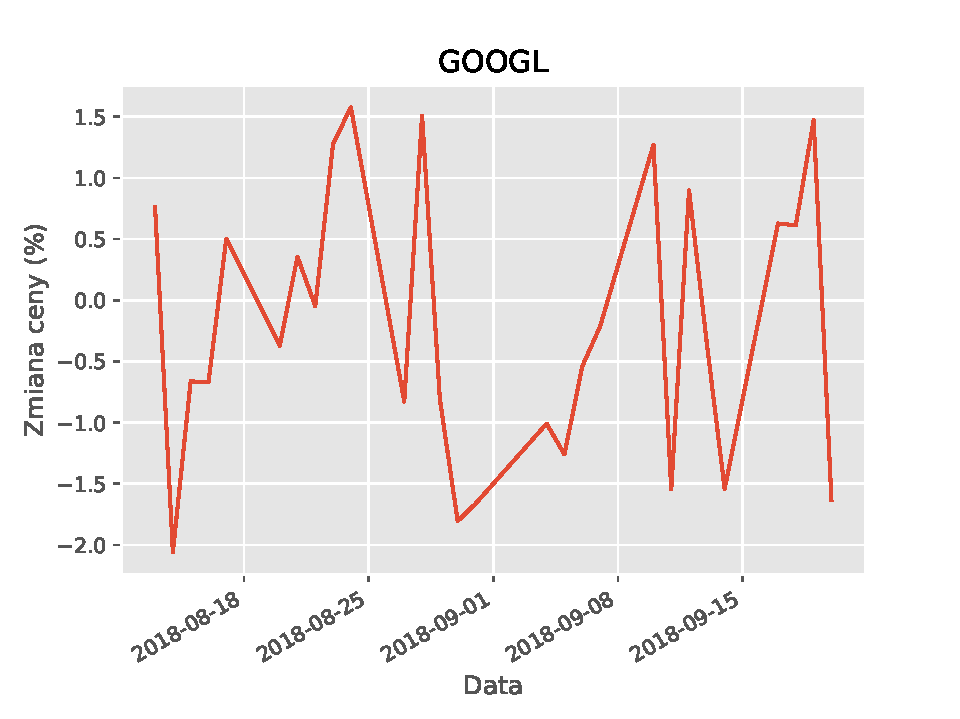
\includegraphics[scale=0.9]{img/googl_pct_change_last_30}
\caption{Dzeinna zmiana ceny akcji spółki \textit{GOOGL} z 30 dni (opracowanie własne)}
\label{img:googl_pct_change_last_30}
\end{figure}

\subsection{Kryteria oceny modeli predykcji}

Porównywanie jakości i wydajności jest nierozłącznym elementem tworzenia i testowania metod uczenia maszynowego. Istnieje wiele sposobów na realizację tego nietrywialnego zadania, które jak się okazuje, często wymaga porównywania modeli na kilku płaszczyznach. Najpopularniejszymi miarami porównawczymi są:
\begin{itemize}
\item procent prawidłowych klasyfikacji
\item pole AUC pod krzywą ROC
\item częściowy indeks Gini
\item metryka F1
\item współczynnik Briera
\item statystyka Kołomogrowa-Smirnova
\end{itemize}

\subsubsection{Macierz błędu}

W przypadku klasyfikacji dwuklasowej na klasy A i B każdą predykcję można przypisać do jednej z 4 grup:
\begin{itemize}
\item True Positive (TP) - gdy przewidziano klasę A dla etykiety A
\item False Negative (FN) - gdy przewidziano klasę B dla etykiety A
\item False Positive (FP) - gdy przewidziano klasę A dla etykiety B
\item True Negative (TN) - gdy przewidziano klasę B dla etykiety B
\end{itemize}

Graficzną reprezentację podziału klasyfikacji na powyższe kategorie nazywamy \textit{macierzą błędu}. Zastosowanie miar opartych o tablicę błędów dla problemów z większą liczbą klas wymaga dodatkowych kroków. W celu policzenia wartości TP, FN, FP i TN należy wyróżnić konkretną klasę, a pozostałe klasy należy zagregować w sztuczną klasę przeciwną. W ten sposób należy wyliczyć konkretną miarę tyle razy ile jest klas. Ostatecznym krokiem w celu uzyskania jednolitej oceny modelu jest na przykład wyliczenie średniej ważonej z wyników dla każdej z klas.


\subsubsection{Procent prawidłowych klasyfikacji}

Jednym z najprostszych sposobów do oceny dokładności klasyfikatorów jest określenie procentu prawidłowych przypisań przykładu do klasy. Metoda ta potrafi dawać złudzenie zadowalających wyników, w których występują duże różnice w licznościach poszczególnych klas. Rozważmy dla takiego zadania naiwny model przypisujący do każdego postawionego przykładu klasę, której liczność jest największa. Wówczas wyniki procentowe prawidłowej klasyfikacji będą wprost proporcjonalne do różnicy w liczności klasy największej w stosunku do innych klas. W większości przypadków pomimo dobrego wyniku taki model będzie uznany za bezużyteczny. Wobec tego tę miarę jakości należy stosować wraz z innymi miarami, które nie są podatne na tego typu zaburzenia.

\subsubsection{Pole AUC pod krzywą ROC}

Krzywa ROC (ang. Receiver Operating Characteristic)\cite{roc} jest narzędziem, która opisuje dokładność klasyfikatora za pomocą oceny jego czułości i precyzji. Precyzją modelu nazywa się stosunek $\frac{TP}{TP+FP}$, zaś czułość jest oznaczona przez $\frac{TP}{TP+FN}$.

\bigskip

Zdefiniujmy wartości \textit{True Positive Rate (TPR)} oraz \textit{False\ Positive\ Rate (FPR)}:

\numberwithin{equation}{subsubsection}

\begin{equation}
TPR = \frac{TP}{TP+FN}
\end{equation}
\begin{equation}
FPR = \frac{FP}{FP+TN}
\end{equation}

Klasyfikatory w większości przypadków nie zwracają dokładnego wyniku przypisania przykładu do klasy. Zazwyczaj wynikiem klasyfikacji jest liczba rzeczywista z przedziału $[0, 1]$, którą można identyfikować jako prawdopodobieństwo. Można przyjąć że jeżeli klasyfikator zwróci $0$ oznacza to przypisanie do klasy A, zaś $1$ oznacza przypisanie do klasy B. Dla wartości z zakresu $(0, 1)$ przypisuje się pewną wartość progową rozgraniczającą obie klasy. Dla tego progu mniejsze od niego wartości przypisujemy do klasy A, zaś resztę do klasy B. Intuicyjnie jest to zazwyczaj połowa przedziału czyli $0.5$.

Krzywa ROC jest graficzną reprezentacją skuteczności modelu klasyfikacyjnego. Jest ona skonstruowana poprzez wykreślenie stosunku $TPR$ do $FPR$ dla różnych progów rozgraniczających klasy. Na rysunku \ref{img:roc} widać przykładowe krzywe ROC dla klasyfikatorów różnej jakości.


%source: https://towardsdatascience.com/understanding-auc-roc-curve-68b2303cc9c5
\begin{figure}[H]%
\centering
\subfigure[Krzywa ROC dla modelu, który nie jest w stanie rozdzielić klas]{%
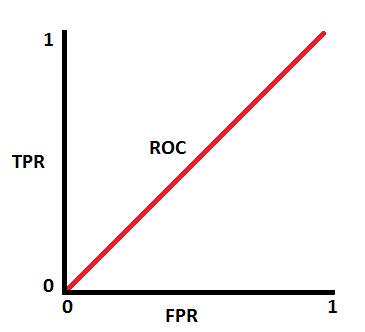
\includegraphics[scale=0.55]{img/roc_1.png}}%
\qquad
\subfigure[Krzywa ROC przykładowego klasyfikatora]{%
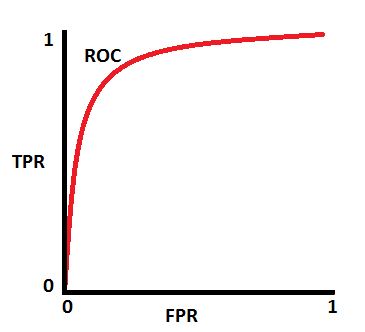
\includegraphics[scale=0.55]{img/roc_2.png}}%
\qquad
\subfigure[Krzywa ROC dla modelu idealnego]{%
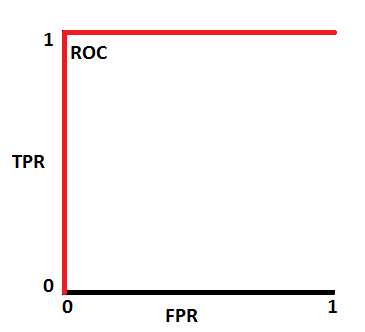
\includegraphics[scale=0.55]{img/roc_3.png}}%
\caption{Przykładowe krzywe ROC \cite{roccurves} }% (źródło: https://towardsdatascience.com/understanding-auc-roc-curve-68b2303cc9c5).}
\label{img:roc}
\end{figure}


Porównanie różnych klasyfikatorów za pomocą krzywej ROC odbywa się poprzez porównanie pola pod krzywymi czyli AUC (ang. Area Under the Curve). Im większe pole pod krzywą ROC dla danego klasyfikatora tym lepsza jest jego jakość. Pole pod krzywą dla modelu idealnego wynosi $1$, zaś dla modelu losowego $0.5$. Warto zauważyć że dla wartości pola poniżej 0.5  korzystnym zabiegiem jest zamiana przedziałów dla klas.

\subsubsection{F1}

Metryka F1 jest średnią harmoniczną metryk czułości i precyzji (wyrażona wzorem $F1=2*\frac{precyzja*czulosc}{precyzja+czulosc}$). Metryka ta jest dobrym narzędziem pozwalającym określić za pomocą jednej wartości jakość modelu, biorąc pod uwagę precyzję jak i czułość modelu. Osiąga ona w najlepszym przypadku wartość 1, zaś w najgorszym wartość 0. 

\subsubsection{Współczynnik Briera}

Współczynnik Briera (ang. Brier score)\cite{brier} jest metodą oceny modeli klasyfikujących opisana wzorem:

$$	BS=\frac{1}{N} \sum_{t=1}^{N} \sum_{i=1}^{R}(f_{ti}-o_{ti})^2 $$

\begin{itemize}
\item $N$ to liczba predykcji,
\item $R$  to liczba możliwych klas
\item $f_{ti}$ to prawdopodobieństwo, które wyznaczył klasyfikator, przypisania przykładu $t$ do klasy $i$,
\item $o_{ti}$ to rzeczywiste przypisanie przykładu do danej klasy (0 gdy przykład nie jest tej klasy, oraz 1 gdy przykład należy do tej klasy).
\end{itemize}

W związku z powyższą definicją, miara ta może zostać wykorzystana w przypadku modeli, które na swoim wyjściu zwracają prawdopodobieństwo przypisania przykładu do każdej z klas. Wobec tego nie każdy model można ocenić tą metryką. Istotnym spostrzeżeniem jest fakt iż w przeciwieństwie do innych metryk, współczynnik Briera modelu idealnego wynosi $0$, zaś im gorszy model tym większy współczynnik.

\subsubsection{Statystyka Kołmogorowa-Smirnova}

Statystyka Kołmogorowa-Smirnova (ang. Kolmogrow-Smirnov Test) \cite{kolsmirtest} pozwala ocenić jakość klasyfikatora binarnego na podstawie stopnia separacji rozkładu dwóch klas. Ocena dokonywana jest przez zmierzenie maksymalnej odległości między wkyresami dystrybuant rozkładu jednej i drugiej klasy. Niech $F(x)$ to dystrybuanta rozkład klasy 1, zaś $G(x)$ to dystrybuanta rozkładu klasy 2. Wówczas statystyka Kołmogorowa-Smirnova opisana jest wzorem:

$$D_{n,m}=\sup_x|F(x)-G(x)|$$

Metryka ta daje wartość 100 dla modelu idealnego, zaś 0 dla modelu losowego.

\subsubsection{Dobór metryki}

Porównanie modeli klasyfikujących jest zadaniem trywialnym tylko dla specyficznych problemów. W tych przypadkach można wykorzystać procent prawidłowych klasyfikacji jako jedyną miarę jakości modeli. W bardziej złożonych przypadkach, gdy dochodzi do dysproporcji w licznościach klas, ta podstawowa miara zostaje w pewien sposób zafałszowana. Innym aspektem, który może być brany pod uwagę przy ocenie klasyfikatorów jest różnica w wadze błędu z grupy \textit{FP}, względem błędu z grupy \textit{FN}. Te problemy należy rozwiązywać poprzez używanie różnorodnych miar do porównywania modeli. Używanie wielu metryk może być przydatne w szczególności gdy dwa modele mają podobne wartości dla jednej z miar.

\bigskip

W zagadnieniu predykcji giełdowych sprowadzonym do klasyfikacji, można posłużyć się \textit{procentem prawidłowych klasyfikacji} jako podstawową miarą porównawczą. Wynika to z faktu, iż dla większości spółek różnica w licznościach klas mieści się w granicach kilku do kilkunastu procent całego zbioru danych. Taka dysproporcja jest jednak na tyle znacząca, że dla porównywania modeli o bliskich wynikach trzeba stosować dodatkową miarę porównawczą. Ze względu na niewrażliwość na dysproporcje w licznościach klas oraz swoją popularność, jako drugą metrykę wykorzystano \textit{pole AUC pod krzywą ROC}.


\subsection{Uczenie modeli - specyfika szeregów czasowych}

Każdy proces uczenia modeli sztucznej inteligencji zwieńczony jest analizą jakości. Zazwyczaj taką analizę przeprowadza się poprzez wydzielenie pewnej części zbioru danych i oznaczenia jej jako zbioru testowego. Reszta zbioru danych zwana jest zbiorem treningowym (rysunek \ref{img:train_test_split}). Taki podział wszystkich próbek pozwala na używanie części treningowej do nauki modelu, zaś części testowej do jego oceny. Ocena modelu na podstawie próbek, któych model nie widział podczas procesu uczenia daje wiarygodne wyniki.

\begin{figure}[H]
\centering 
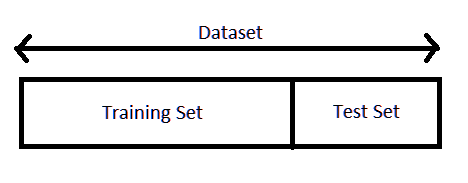
\includegraphics[scale=0.5]{img/train_test_split.png}
\caption{Podział danych na zbiór treningowy i testowy \cite{train_test_split}}
\label{img:train_test_split}
\end{figure}

Ten model podziału jest najbardziej powszechny pośród zagadnień klasyfikacyjnych ze względu na swoją prostotę i odporność na zjawisko przeuczenia (ang. overfitting). Dane giełdowe jako szeregi czasowe posiadają dodatkową cechę - umiejscowienie próbek na osi czasu. Wykorzystanie faktu, iż kolejne próbki danych pojawiają się stopniowo wraz z upływem czasu, pozwala na udoskonalenie metody doboru danych do uczenia się. Uczenie i ocena metodą kroczącą (ang. walk forward) polega na stopniowym powiększaniu zbioru danych treningowych o kolejne próbki ze zbioru testowego podczas procesu oceny jakości. 

\textit{Przykład:} podczas oceny jakości model przewiduje cenę za pomocą próbki z dnia $t$ mając do uprzedniej nauki wszystkie próbki od $t_0$ do $t-1$. Po tej predykcji próbka z dnia $t$ zostaje wcielona do zbioru uczącego. Model może, ale nie musi, zostać ponownie poddany procesowi uczenia przed przystąpieniem do oceny jakości dla predykcji kolejnej próbki $t+1$. Proces ten zobrazowany jest na rysunku \ref{img:train_test_split_time_series}. Na niebiesko oznaczono próbki zbioru treningowego, na czerwono zaś próbkę zbioru testowego podlegającą ocenie.

\begin{figure}[H]
\centering 
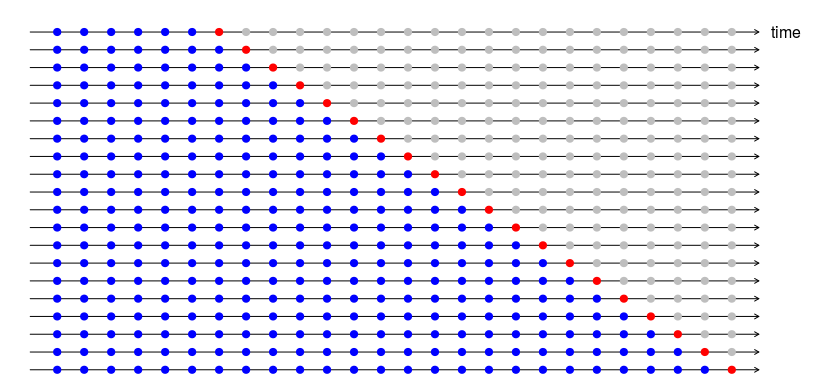
\includegraphics[scale=0.75]{img/train_test_split_time_series.png}
\caption{Podział danych na zbiór treningowy i testowy metodą kroczącą \cite{train_test_split_time_series}}
\label{img:train_test_split_time_series}
\end{figure}

Wykorzystanie metody kroczącej do podziału zbioru danych pozwala zmaksymalizować ilość informacji przekazanych do modelu podczas procesu uczenia, a tym samym poprawia końcowe wyniki klasyfikacji. 


\subsection{Wnioski i uwagi}

Do zagadnienia predykcji cen na giełdzie można podchodzić na kilka sposobów. Najbardziej intuicyjnym rozwiązaniem z perspektywy początkującego inwestora, jest model, który na wyjściu wyznacza jaką akcję powinien wykonać inwestor w stosunku do akcji konkretnej spółki. Doświadczony makler do wyznaczania cen zapewne wybrałby model regresyjny, który poza określeniem trendu daje możliwość oceny jak duże są wahania ceny. Dzięki temu mógłby dobrać spółki, dla których wzrost cen będzie największy. Przy ocenie jakości regresji błąd jest zazwyczaj określany za pomocą odległości przewidywanej wartości ceny od rzeczywistej wartości ceny. Informacja że dany model aproksymuje wartość ceny z błędem $\pm 5 \$$ jest ciężka do zinterpretowania wprost. Na podstawie takiej oceny makler nie jest w stanie bezpośrednio stwierdzić czy taki model nadaje się do użycia na giełdzie. Dla zagadnienia klasyfikacji błąd jest określony jako $\%$ prawidłowych klasyfikacji, więc daje dużo lepsze wyobrażenie na temat jakości i możliwości wykorzystania modelu do obrotu akcjami.

\bigskip



\newpage

\section{Analiza i przetwarzanie danych}

Przed przystąpieniem do wyboru modeli należy zastanowić się nad danymi jakie będą służyć do ich uczenia. Wybór odpowiednich cech, analiza zebranych informacji oraz przetworzenie ich, wykracza poza zakres uczenia maszynowego tworząc własną dziedzinę zwaną inżynierią i analizą danych. Odpowiedni dobór i obróbka danych wejściowych często daje większe korzyści niż dopracowywanie modeli przewidujących i optymalizacja ich parametrów. 

\subsection{Wybrane cechy}

Spośród dostępnych danych do uczenia modeli wybrane zostały: 
\begin{itemize}
\item podstawowe dane giełdowe oraz ich modyfikacje,
\item wybrane wskaźniki analizy technicznej oraz ich modyfikacje.
\end{itemize}

Analiza fundamentalna ze względu na swoją długoterminową naturę (raporty finansowe spółek publikowane kwartalnie) jest mało istotna przy dziennych predykcjach giełdowych. Dodatkowo istnieje mało darmowych źródeł danych analizy fundamentalnej. Z tych względów zostanie ona pominięta w tej pracy.

\bigskip

Wszystkie dane wejściowe, wraz z opisami, zaprezentowane są w tabeli \ref{tab:data_columns_table}. Wszystkie dane mają charakter dzienny. Najnowsze informacje pochodzą z dnia \textit{t}, zaś przewidywaną ceną jest cena z dnia \textit{t+1}.

\begin{longtable}[c]{| m{0.5cm} m{5cm} m{10cm}|} 

\toprule
  Lp. & Oznaczenie & Opis\\
\midrule
\endhead
\midrule

\caption{Wybrane cechy i ich opis}
\label{tab:data_columns_table}
\endfoot

\bottomrule
\caption{Wybrane cechy i ich opis}
\label{tab:data_columns_table}
\endlastfoot


 1 & $C_t$ & Cena zamknięcia w dniu $t$. \\ 
 2 & $O_t$ & Cena otwarcia w dniu $t$. \\
 3 & $H_t$ & Najwyższa cena w dniu $t$. \\
 4 & $L_t$ & Najniższa w dniu $t$. \\
 5 & $V_t$ & Liczba akcji w obrocie w dniu $t$. \\
 6 & $HL\_PCT$ & Różnica pomiędzy $H_t$ a $L_t$ wyrażona w procentach.\\
 7 & $SMA_5$ & Średnia krocząca z 5 dni. \\
 8 & $SMA_{10}$ & Średnia krocząca z 10 dni. \\\
  9 & $SMA_{20}$ & Średnia krocząca z 20 dni. \\
 10 & $SMA\_DIFF$ & $SMA_{10}-SMA_{5}$ \\
 11 & $SMA\_DIFF2$ & $SMA_{20}-SMA_{5}$ \\
 12 & $TR$ & (ang. True Range) różnica pomiędzy najniższą ceną, a najwyższą ceną danego dnia. \\
 13 & $MACD$ & Wskaźnik wyliczany z różnicy dwóch wykładniczych średnich kroczących.\\
 14 & $MACD\_SIGNAL$ & Wykładnicza średnia krocząca ze wskaźnika MACD \\
 15 & $ROC_{5}$ & (ang. Rate of Change) Wskaźnik liczący procentową różnicę w cenie między dniem $t$ a $t-5$. \\
 16 & $ROC_{10}$ & (ang. Rate of Change) Wskaźnik liczący procentową różnicę w cenie między $t$ a $t-10$. \\
 17 & $ROC\_DIFF$ & $ROC_{10}-ROC_{5}$ \\
  18 & $MOM_{5}$ & Momentum - różnica w cenie między $t$ a $t-5$.  \\
 19 & $MOM_{10}$ & Momentum - różnica w cenie między $t$ a $t-10$. \\
 20 & $MOM\_DIFF$ & $MOM_{10}-MOM_{5}$ \\
  21 & $WILLR_{5}$ & \textit{Williams` \%R} - wskaźnik niedosycenia/przesycenia ceny z ostatnich 5 dni. \\
 22 & $WILLR_{10}$ & \textit{Williams` \%R} - wskaźnik niedosycenia/przesycenia ceny z ostatnich 10 dni.  \\
 23 & $WILLR\_DIFF$ & $WILLR_{10}-WILLR_{5}$ \\
  24 & $APO_{5}$ & Oscylator ceny z 5 dni. \\
 25 & $APO_{10}$ & Oscylator ceny z 10 dni.  \\
 26 & $APO\_DIFF$ & $APO_{10}-APO_{5}$ \\
  27 & $RSI_{5}$ & Wskaźnik siły względnej - oscylator siły trendu z 5 dni. \\
 28 & $RSI_{10}$ & Wskaźnik siły względnej - oscylator siły trendu z 10 dni.\\
 29 & $RSI\_DIFF$ & $RSI_{10}-RSI_{5}$ \\
  30 & $ADX_{5}$ & Wskaźnik siły trendu z 5 dni. \\
 31 & $ADX_{10}$ & Wskaźnik siły trendu z 10 dni. \\
 32 & $ADX\_DIFF$ & $ADX_{10}-ADX_{5}$ \\
 33 & $CCI_{5}$ & (ang. Commodity Channel Index) Oscylator z 5 dni. \\
 32 & $CCI_{10}$ & (ang. Commodity Channel Index) Oscylator z 10 dni. \\
 34 & $CCI\_DIFF$ & $CCI_{10}-CCI_{5}$ \\
 35 & $AD$ & linia \textit{Chaikin A/D}.  \\
 36 & $STOCH\_K$ & Oscylator stochastyczny \textit{Slow \%K}. \\
 37 & $STOCH\_D$ & Oscylator stochastyczny \textit{Slow \%D}.\\
 39 & $STOCH\_K\_DIFF$ & $STOCH\_K_{t}-STOCH\_K_{t-1}$ \\
 40 & $STOCH\_D\_DIFF$ & $STOCH\_D_{t}-STOCH\_D_{t-1}$  \\
 41 & $DISPARITY_{5}$ &  $\frac{C_t}{SMA_5}\times 100$ \\
 42 & $DISPARITY_{10}$ & $\frac{C_t}{SMA_10}\times 100$ \\
 43 & $DISPARITY_{20}$ & $\frac{C_t}{SMA_20}\times 100$ \\
 44 & $BANDS\_DIFF_{10}$ & $BOLL\_UP_{10} - BOLL\_LOW_{10}$ - różnica górnej i dolnej wartości wstąg Bollingera z 10 dni.  \\
 45 & $BANDS\_DIFF_{20}$ & $BOLL\_UP_{20} - BOLL\_LOW_{20}$ - różnica górnej i dolnej wartości wstąg Bollingera z 20 dni.  \\
46 & $PRICE\_BANDS\_UP_{10}$ & $(C_t-BANDS\_UP_{10})\div BANDS\_UP_{10}$ - wskaźnik oparty o wstęgi Bollingera.  \\
 47 & $PRICE\_BANDS\_LOW_{10}$ & $(C_t-BANDS\_LO_{10})\div BANDS\_LOW_{10}$ - wskaźnik oparty o wstęgi Bollingera.\\
 48 & $PRICE\_BANDS\_UP_{20}$ & $(C_t-BANDS\_UP_{20})\div BANDS\_UP_{20}$ - wskaźnik oparty o wstęgi Bollingera.\\
 49 & $PRICE\_BANDS\_LOW_{20}$ & $(C_t-BANDS\_LOW_{20})\div BANDS\_LOW_{20}$ - wskaźnik oparty o wstęgi Bollingera.\\
     
\end{longtable}

\subsection{Przetwarzanie wstępne}

Po wybraniu odpowiednich danych należy przystąpić do ich pobrania. Pobrane dane nie są jednak gotowe do wykorzystania w procesie uczenia maszynowego. Zbiory informacji, w szczególności te pobrane z internetu, należy traktować zgodnie z zasadą ograniczonego zaufania. Wobec braku gwarancji jakości, dane powinny zostać zbadane pod względem integralności oraz poprawności. Spośród najczęstszych problemów wymienić można: 
\begin{itemize}
    \item brakujące informacje,
    \item duplikacja danych,
    \item dane nominalne (np. łańcuchy znaków),
    \item błędy pomiarowe.
\end{itemize}

W celu eliminacji błędnych danych należy je usunąć lub zastąpić wybraną wartością np. średnią wartością z danej cechy. Jeśli chodzi o dane nominalne stosowana jest \textbf{binaryzacja}. Polega ona na odpowiednim przekształceniu cechy na wektor cyfr. Po wyeliminowaniu powyższych problemów dane warto przetworzyć takimi metodami jak \textbf{normalizacja} czy \textbf{standaryzacja}. Służą one do przeskalowania zakresu możliwych wartości do przedziału $[0,1]$ lub $[-1,1]$. Taki zabieg polepsza wydajność modeli uczenia maszynowego.

\bigskip

\subsubsection{Niestacjonarność szeregów czasowych}

Na rysunku \ref{img:non_stationary_adjusted_close} zauważyć można zjawisko niestacjonarności. Jest to cecha związana z autokorelacją zmiennych szeregów czasowych. Oznacza to iż kolejne wyrazy szeregu zależą w jakimś stopniu od poprzednich. Dla cen akcji ta zależność jest ewidentna, cena każdego dnia jest oparta o cenę z dnia poprzedniego. 

\begin{figure}[H]
\centering 
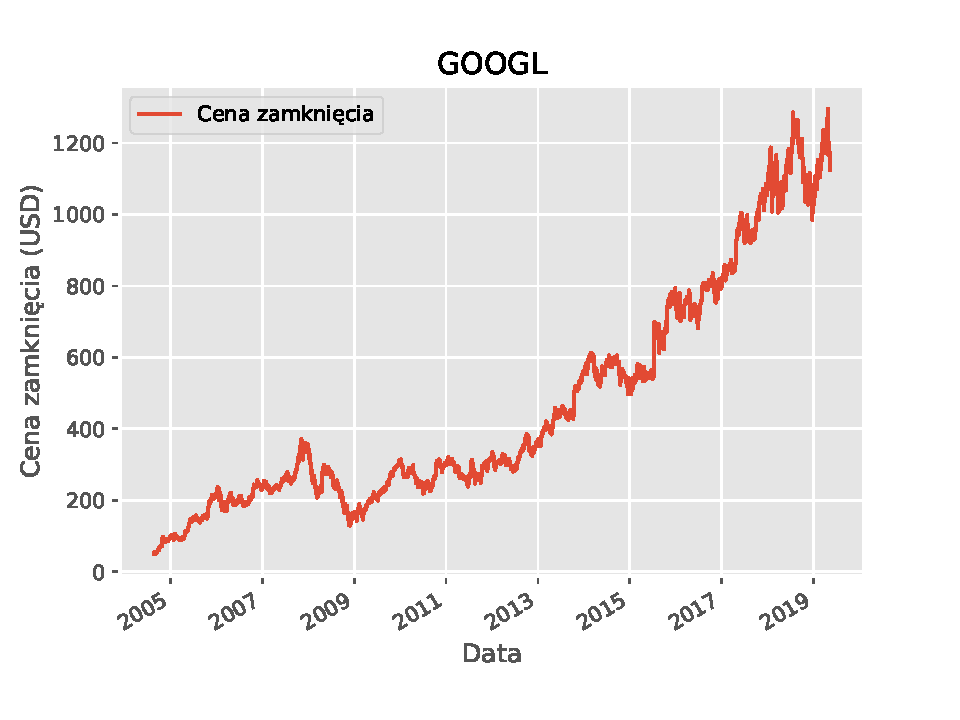
\includegraphics[scale=0.9]{img/GOOGL_adj_close.pdf}
\caption{Wykres cen akcji spółki \textit{Alphabet Inc} (opracowanie własne)}
\label{img:non_stationary_adjusted_close}
\end{figure}

Zjawisko niestacjonarności szeregów czasowych negatywnie wpływa na wykorzystywanie ich do uczenia maszynowego. Wszystkie zmienne, których dotyczy ten problem trzeba odpowiednio dostosować przed użyciem do uczenia modeli. Najbardziej powszechną metodą radzenia sobie z niestacjonarnością jest różnicowanie (ang. \textbf{differencing}). Jest to prosta metoda polegająca na wyliczeniu różnicy pomiędzy kolejnymi elementami w szeregu. W ten sposób zmienna $x_t$ jest zastąpiona przez $x'_t=x_t-x_{t-1}$. Wynik takiego przetworzenia dla ceny zamknięcia spółki \textit{Alphabet Inc} widoczny jest na rysunku \ref{img:stationary_adjusted_close}.

%TODO zamienić na tabelki

\begin{figure}[H]
\centering 
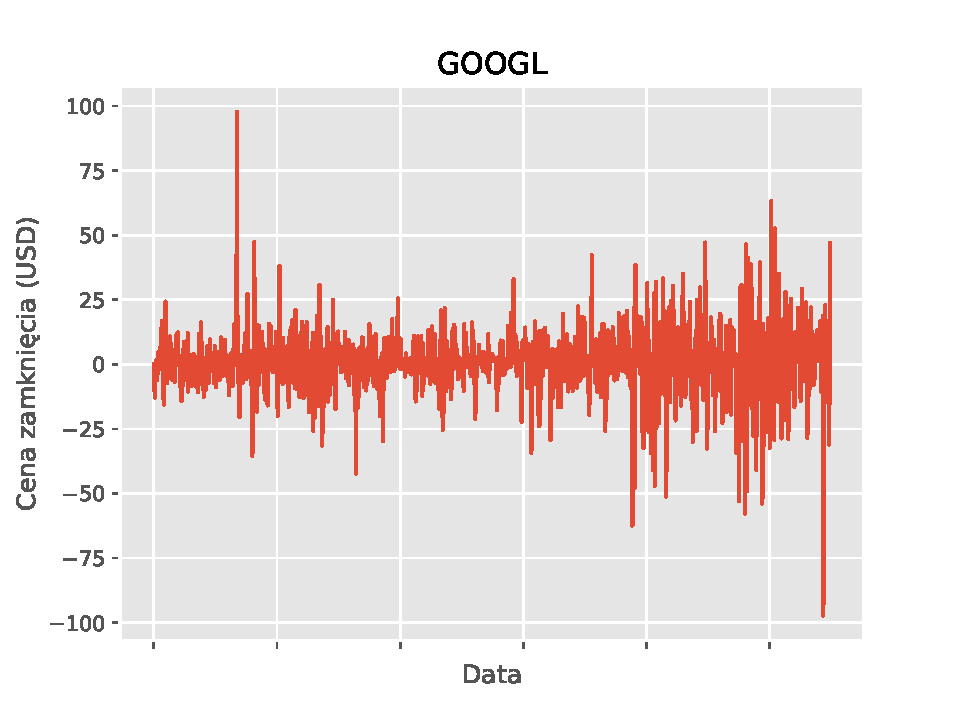
\includegraphics[scale=0.9]{img/adjusted_close_stationary.pdf}
\caption{Wykres cen akcji spółki \textit{Alphabet Inc} po przetworzeniu (opracowanie własne)}
\label{img:stationary_adjusted_close}
\end{figure}

\subsubsection{Wyznaczenie etykiet}

W procesie nadzorowanego uczenia maszynowego poza danymi wejściowymi potrzeba również etykiet, tj. zbioru pożądanych odpowiedzi. W przypadku regresyjnej predykcji cen zamknięcia w dniu $t$ etykietą jest cena zamknięcia z dnia $t+1$. Etykietę dla każdego wiersza danych wejściowych można więc uzyskać poprzez dodanie kolumny ceny zamknięcia przesuniętej o jeden dzień wstecz (zilustrowane na rysunku \ref{img:regression_label_creation}). 

\begin{figure}[H]
\centering 
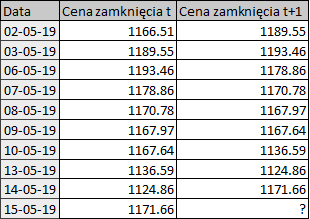
\includegraphics[scale=0.9]{img/label_creation.png}
\caption{Przykładowe dane dla spółki \textit{Alphabet Inc}}
\label{img:regression_label_creation}
\end{figure}

W celu osiągnięcia etykiet do klasyfikacji potrzeba wykonać dodatkowe kroki. Korzystając z nowej kolumny można obliczyć różnicę pomiędzy $C_t$, a $C_{t+1}$ . Wyznaczenie etykiety trendu do klasyfikacji binarnej sprowadza się do wyliczenia funkcji $sgn(C_{t+1}-C_{t})$ (rysunek \ref{img:binary_label_creation}). 

\begin{figure}[H]
\centering 
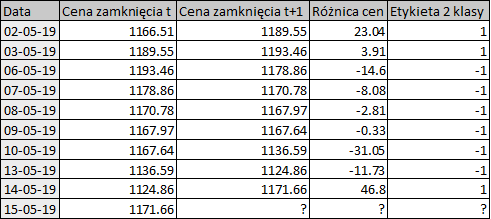
\includegraphics[scale=0.9]{img/label_creation2.png}
\caption{Przykładowe dane dla spółki \textit{Alphabet Inc}}
\label{img:binary_label_creation}
\end{figure}

 W przypadku klasyfikacji podzielonej na 3 klasy wyznaczenie etykiety sprowadza się do obliczenia procentowej różnicy pomiędzy cenami zamknięcia - $100*(C_{t+1}-C_t)/C_t$. Tak wyliczoną różnicę procentową można wykorzystać do przypisania etykiecie wartości $-1, 0, 1$ w zależności od wybranego progu opłacalności. Przykładowe obliczenia zostały zilustrowane na rysunku \ref{img:classification_label_creation}.

\begin{figure}[H]
\centering 
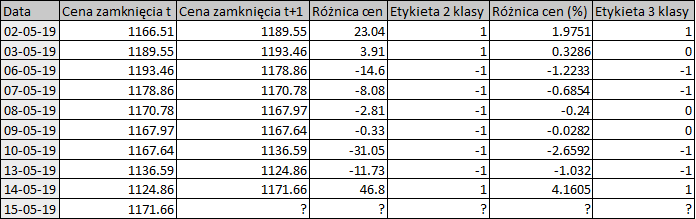
\includegraphics[scale=0.9]{img/label_creation3.png}
\caption{Przykładowe dane dla spółki \textit{Alphabet Inc}}
\label{img:classification_label_creation}
\end{figure}

\subsubsection{Redukcja danych wejściowych}

Redukcja rozmiaru danych wejściowych jest zagadnieniem pozwalającym na poradzenie sobie ze zbyt dużą liczbą danych wejściowych. Jeżeli dwie zmienne są ze sobą mocno skorelowane, wówczas jedną z nich można odrzucić bez utraty zawartych w niej informacji. Macierz korelacji par zmiennych wejściowych przedstawiona jest na rysunku \ref{img:correlation}. Analizując macierz korelacji zauważyć można że duża część zmiennych jest ze sobą mocno skorelowana (wartości bliskie $1$ oznaczają wysoką korelację, 0 brak korelacji, zaś $-1$ negatywną korelację).

\begin{figure}[H]
\centering 
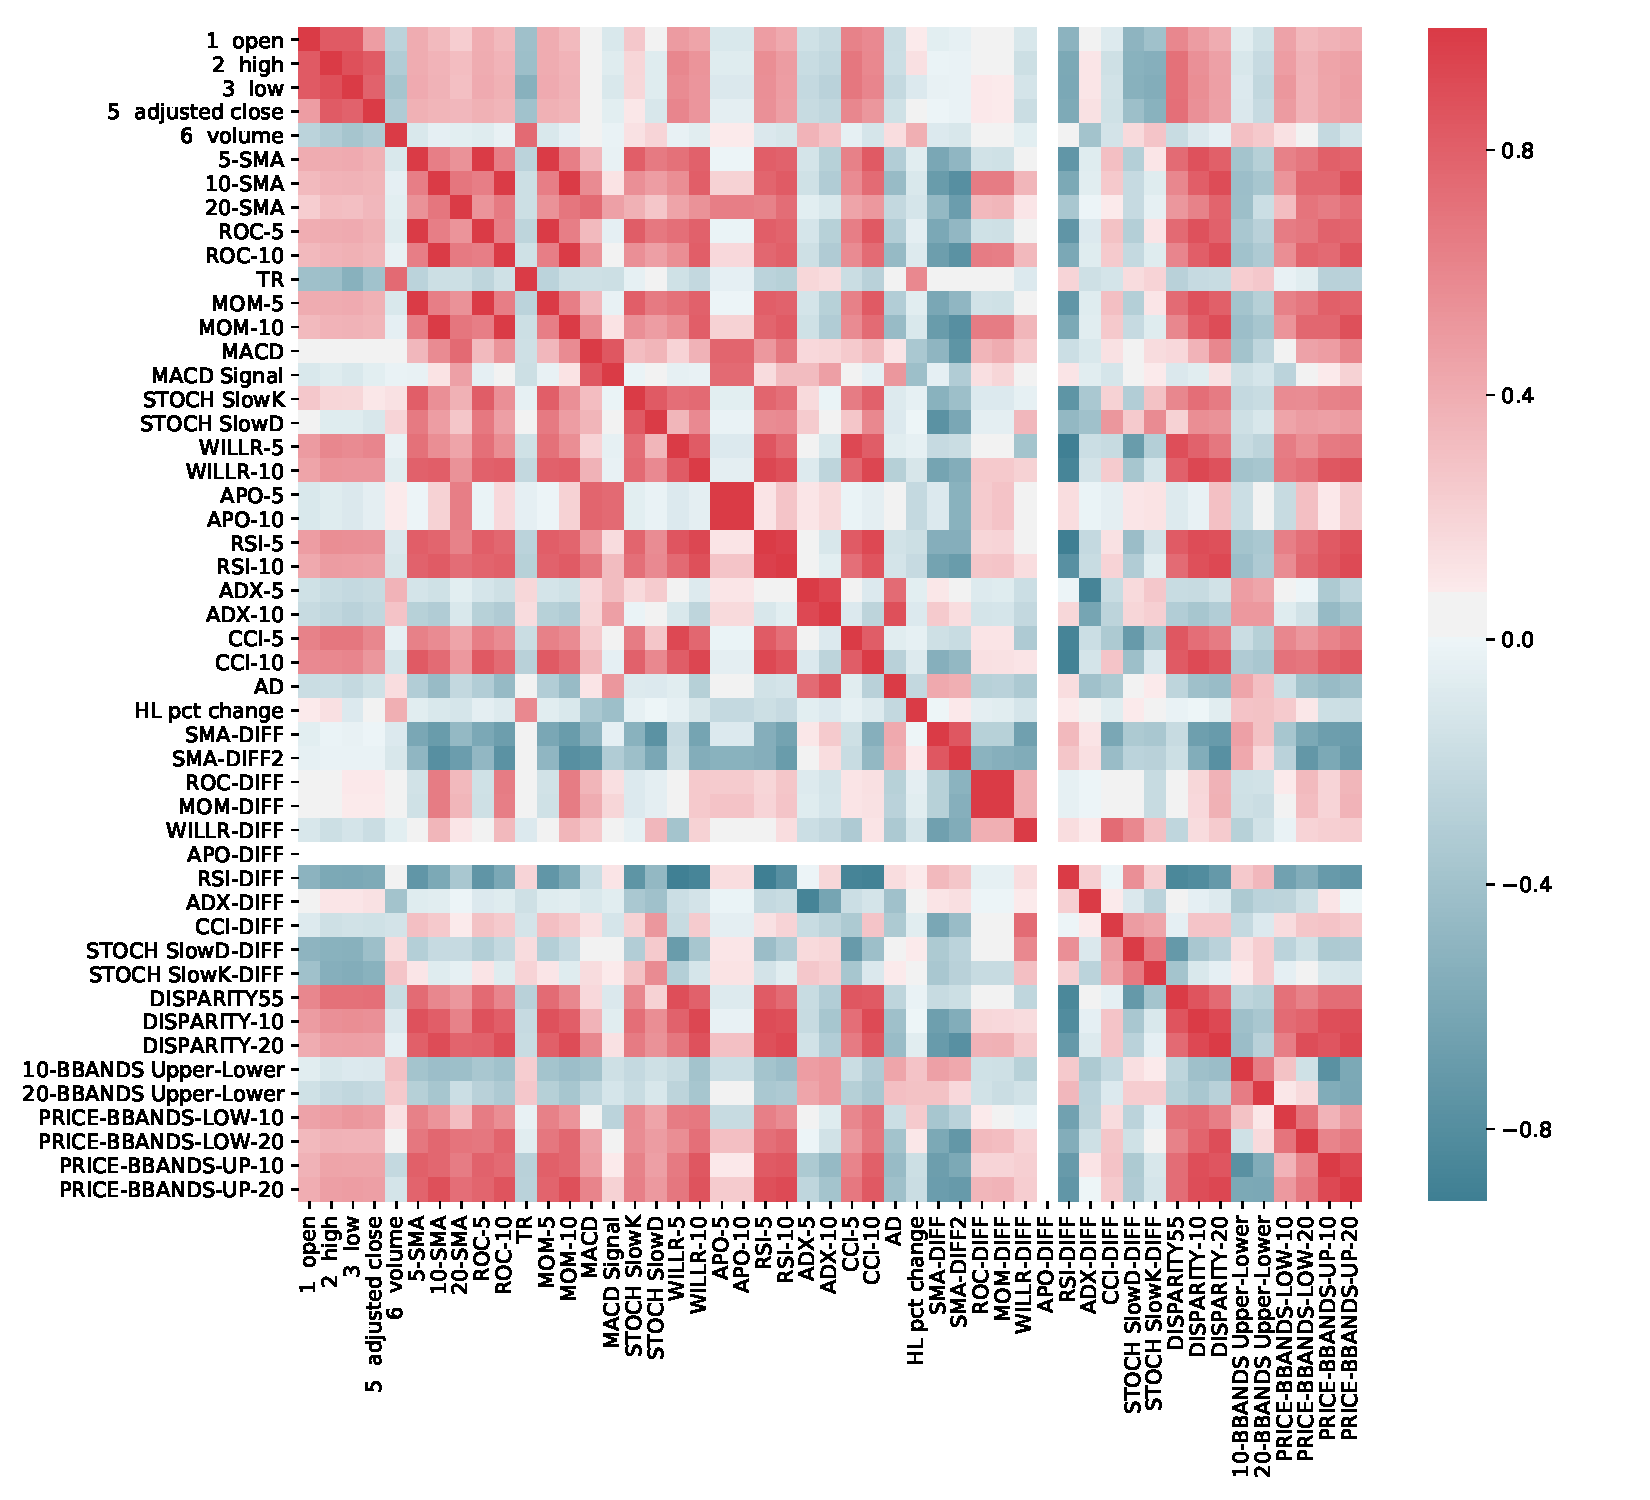
\includegraphics[scale=0.6]{img/corr_matrix.pdf}
\caption{Macierz korelacji par zmiennych (opracowanie własne)}
\label{img:correlation}
\end{figure}

Dla par zmiennych o najwyższej korelacji można usunąć jedną ze zmiennych, ponieważ powiela ona informacje już zawarte w drugiej zmiennej.  W tabeli \ref{tab:ccorr_table1} zostały wylistowane pary zmiennych o najwyższej korelacji. Ze zbioru wejściowego usunięte zostały zmienne z kolumny \textit{Zmienna 2}.


\begin{table}[H]
\centering
\begin{tabular}{ |c|c|c| } 
 \hline
Zmienna 1 & Zmienna 2 &  Stopień korelacji \\
 \hline
APO-5 & APO-10 &  1.000000 \\
 \hline
10-SMA & MOM-10 &  1.000000 \\
 \hline
5-SMA & MOM-5 &  1.000000 \\
 \hline
5-SMA & ROC-5 &  0.997665 \\
 \hline
10-SMA & ROC-10 &  0.996666 \\
 \hline
RSI-5 & RSI-10 &  0.964811 \\  
 \hline
\end{tabular}
\caption{Tabela najbardziej skorelowanych par zmiennych}
\label{tab:ccorr_table1}
\end{table}


Po odrzuceniu najmocniej skorelowanych danych można skorzystać z jednej z metod redukcji wymiaru zadania wejściowego jaką jest \textbf{analiza głównych składowych} (ang. principal component analysis). Jest to statystyczna metoda analizy czynnikowej, która modyfikuje układ współrzędnych w taki sposób aby maksymalizować wariancję kolejncyh zmiennych. Dzięki temu tworzona jest nowa przestrzeń obserwacji, w której najwięcej zmienności przedstawiają początkowe czynniki. Metode ta opiera się o macierz korelacji lub macierz kowariancji stworzonej z danych wejściowych. Rozmiar wejścia redukowany jest poprzez wybranie czynników, które reprezentują największą część wariancji w zbiorze danych. Stosunek liczby wybranych zmiennych do proocenta całkowitej wariancji zbioru danych przedstawiony jest na rysunku \ref{img:pca_variance}. Zawarcie $90\%$ wariancji wymaga użycia 8 składowych,  $95\%$ wariancji wymaga użycia 12 składowych, $99\%$ wariancji wymaga użycia 19 składowych. Wybranie wartości $99\%$ wariancji pozwala ograniczyć rozmiar wejściowego wektora o ponad połowę bez utraty informacji w nim zawartych.

\begin{figure}[H]
\centering 
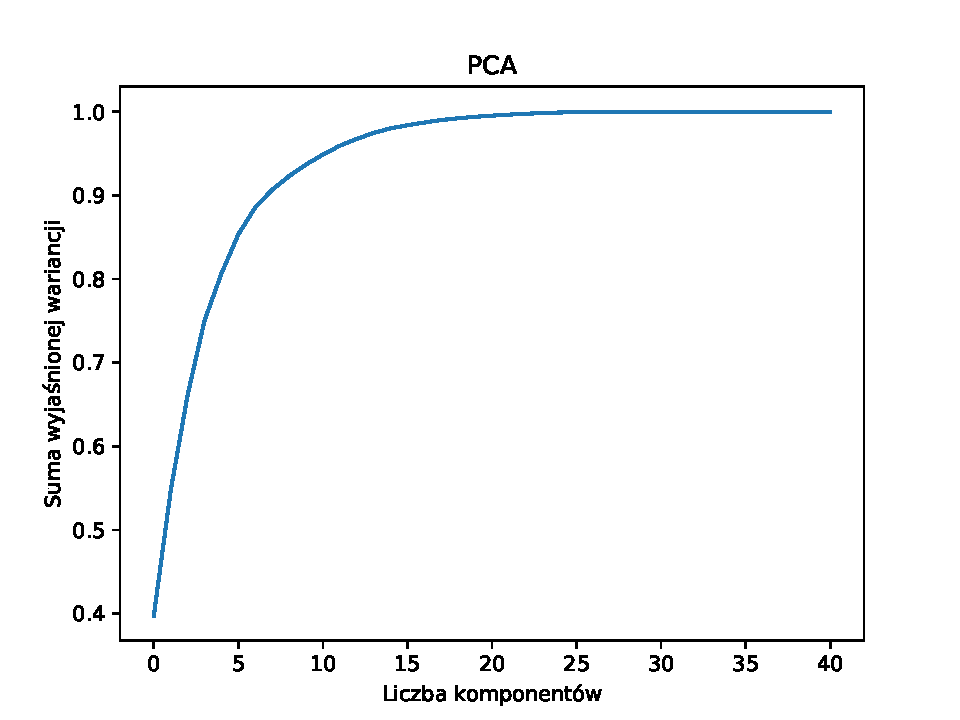
\includegraphics[scale=0.9]{img/pca_variance.pdf}
\caption{Liczba składowych, a całkowita wariancja zbioru (opracowanie własne)}
\label{img:pca_variance}
\end{figure}

\newpage

\section{Wybrane algorytmy do prognozowania}

Istnieje wiele algorytmów mogących posłużyć do zagadnień klasyfikacji lub regresji. W tym rozdziale omówione zostały klasyfikatory, które później zostały użyte do predykcji na danych giełdowych.

\subsection{SVM}

Maszyny wektorów nośnych (ang. Support-Vector Machines)\cite{svm} są zbiorem klasyfikatorów mających na celu wyznaczenie hiperpłaszczyzn rozdzielających klasy z zachowaniem maksymalnego marginesu rozdzielającego (rysunek \ref{img:wiki_svm}). W podstawowej wersji klasyfikatory SVM potrafią sktuecznie klasyfikować problemy separowalne liniowo.


\begin{figure}[H]
\centering 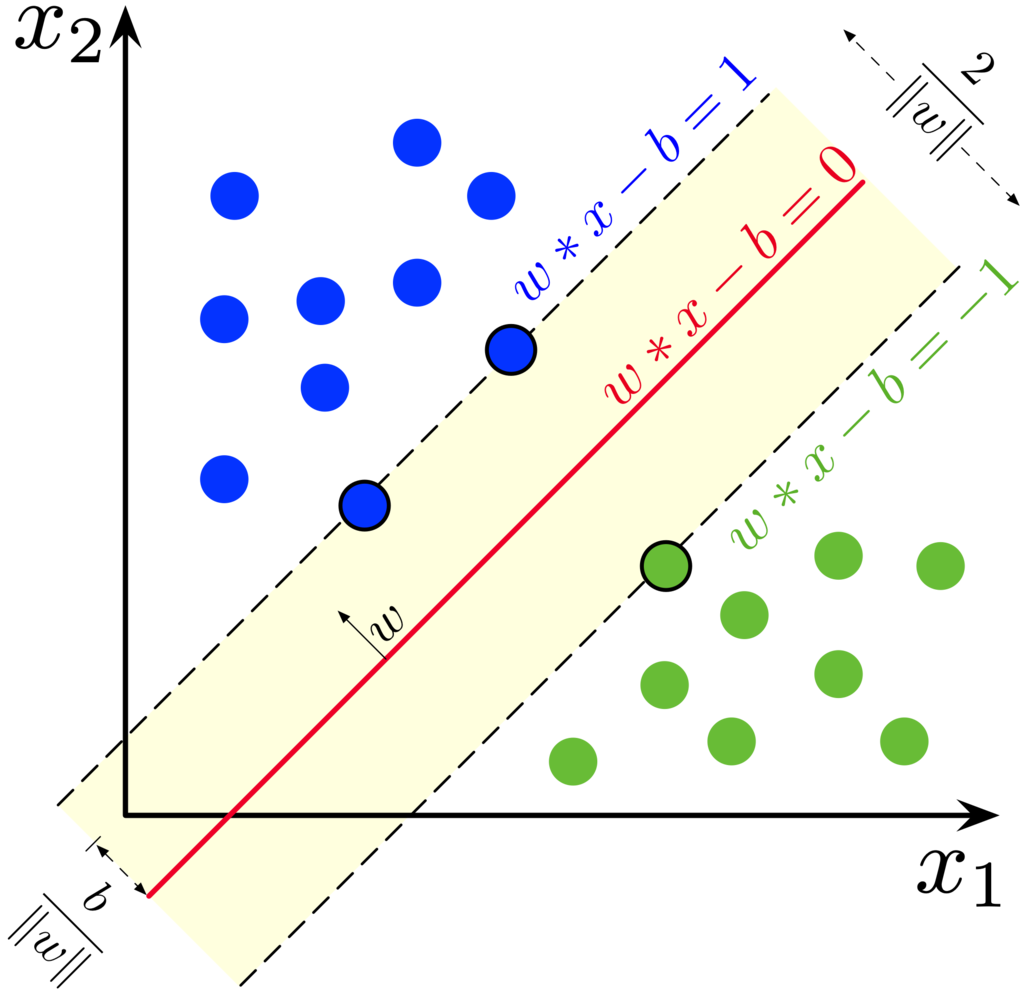
\includegraphics[scale=0.9]{img/svm.png}
\caption{Hiperpłaszczyzna rozdzielająca zbiór z maksymalnym marginesem \cite{wikisvm}}
\label{img:wiki_svm}
\end{figure}

W celu używania maszyn wektorów nośnych do klasyfikacji problemów nieliniowych stosuje się przekształcanie przestrzeni zadania za pomocą funkcji jądrowych. Wprowadzają one dodatkowe wymiary do zadania, w których znalezienie hiperpłaszczyzny rozdzielającej klasy może okazać się prostsze (rysunek \ref{img:wiki_svm2}). Do najpopularniejszych funkcji jądrowych zalicza się funkcje: liniową (zachowującą wymiar zadania w niezmienionym stanie), wielomianową, radialną czy też sigmoidalną.


\begin{figure}[H]
\centering 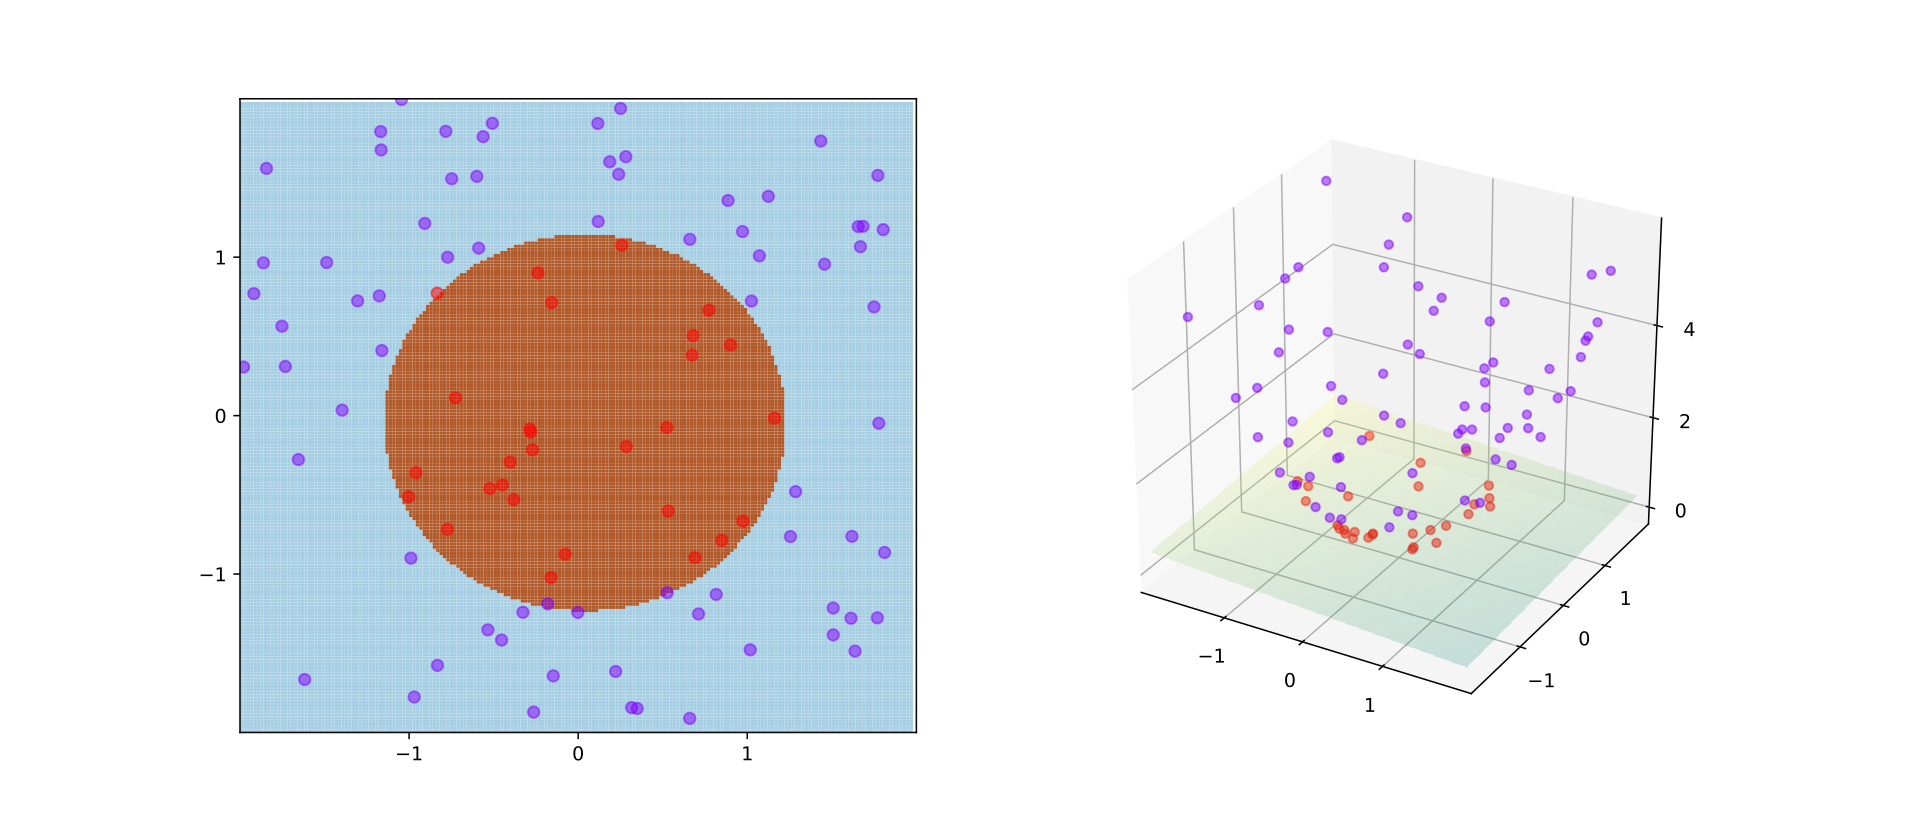
\includegraphics[scale=0.2]{img/svm2.png}
\caption{Ten sam problem zaprezentowany w dwóch oraz trzech wymiarach \cite{wikisvm}}
\label{img:wiki_svm2}
\end{figure}


\subsection{Sztuczne sieci neuronowe}

Sieci neuronowe \cite{neural-nets} są zbiorem modeli matematycznych służących do realizacji obliczeń, bądź przetwarzania sygnałów. Inspirowane działaniem mózgu, swoją nazwę czerpią z upodobnienia struktury do naturalnych neuronów oraz łączących je synaps. Głównymi zastosowaniami sieci neuronowych są zadania regresji, klasyfikacji oraz generowania danych. 

\bigskip

Podstawowym elementem sieci neuronowej jest neuron, który na wejściu przyjmuje dane wejściowe, przetwarza i zwraca pojedynczy sygnał wyjściowy. Przetwarzanie sygnału przez neuron z polega zazwyczaj na zsumowaniu sygnałów dochodzących do niego, a następnie obliczenie wartości funkcji aktywacji. Uzyskana wartość z funkcji aktywacji jest przekazywana jako wyjście z neuronu (rysunek \ref{img:neural-net}). Funkcje aktywacji mogą wprowadzić element nieliniowy do modelu dzięki czemu sieci neuronowe mogą posłużyć do klasyfikacji zbiorów, które nie są separowalne liniowo. Dodatkowo połączenia między neuronami posiadają przypisaną wagę mającą bezpośredni wpływ na wartość sygnału przechodzącego między nimi.

\bigskip

Wiodącym schematem uczenia sieci neuronowych jest korzystanie z przykładów, z których każdy ma etykietę czyli oczekiwaną wartość wyjściową. Każdy z przykładów jest przetwarzany przez sieć neuronową, następnie przez zestawienie wartości wyjściowej sieci z etykietą (odpowiednią funkcją straty) można wyliczyć błąd sieci dla danego przykładu. Ostatnim krokiem jest poprawa wag w sieci neuronowej według wybranej metody propagacji wstecznej. Problem optymalizacji sieci neuronowej sprowadzany jest do problemu optymalizacji funkcji poprzez modyfikację wag na połączeniach między neuronami. Metoda ta zaliczana jest do nauczania z nauczycielem (ang. supervised learning). Najczęściej stosowanymi metodami optymalizacji są algorytmy spadku gradientowego. 

\bigskip

Przy wykorzystywaniu sieci neuronowych głównym problemem, z którym zmagają się naukowcy jest odpowiedni dobór parametrów i algorytmów. Spośród elementów wymagających odpowiedniego dobrania wymienić można następujące:
\begin{itemize}
\item liczba warstw sieci,
\item liczba neuronów w każdej z warstw ukrytych,
\item wykorzystane funkcje aktywacji,
\item algorytm optymalizacyjny,
\item funkcja straty.
\end{itemize}


\subsubsection{Sieci typu MLP}

Jednym z najprostszych przykładów sieci neuronowych jest perceptron wielowarstwowy (ang. multilayer perceptron) \cite{mlp}. Taka sieć składa się z warstwy wejściowej, z dowolnej ilości warstw ukrytych oraz z warstwy wyjściowej. W tym rodzaju sieci neuronowych, sygnał wyjściowy dowolnego neuronu jest traktowany jako sygnał wejściowy każdego z neuronów z kolejnej warstwy (rysunek \ref{img:neural-net}). 

\bigskip

\begin{figure}[H]
\centering 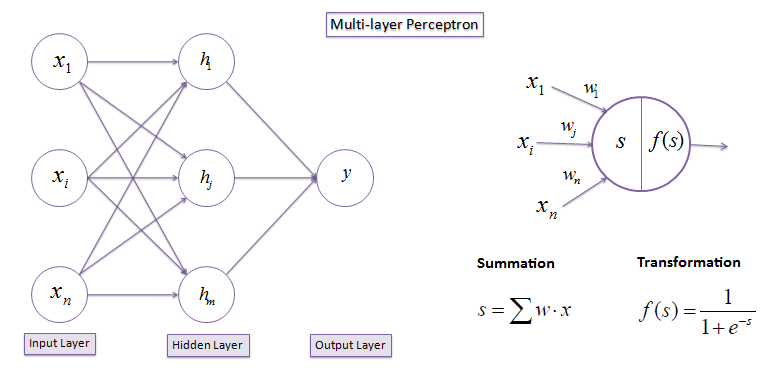
\includegraphics[scale=0.7]{img/nn.png}
\caption{Schemat sieci neuronowej typu MLP \cite{mlpnn}}
\label{img:neural-net}
\end{figure}

Najprostszą implementacja sieci do predykcji danych giełdowych jest sieć przyjmująca na wejściu wektor informacji o akcjach spółki z jednego dnia, zwracająca na wyjściu przewidywaną wartość ceny akcji następnego dnia. Perceptron wielowarstwowy można również zaprojektować tak, aby na wyjściu zwracał wynik klasyfikacji, czyli procentowy wynik przypisania danych wejściowych do każdej z możliwych klas. W tej pracy badane były sieci neuronowe klasyfikujące dane wejściowe według trzech klas: spadek wartości poniżej pewnego progu, utrzymanie wartości w ramach tego progu oraz wzrost wartości powyżej tego progu. 

\subsection{Random forest}

Las losowy (ang. Random Forest)\cite{randforest} jest modelem opartym o drzewa decyzyjne służącym do klasyfikacji lub regresji. Drzewa decyzyjne są graficzną metodą wspomagania procesu decyzyjnego. W przypadku zagadnień uczenia maszynowego drzewa decyzyje najprościej zobrazować na przykładzie problemu klasyfikacji binarnej. Na rysunku \ref{img:wiki_dec_tree} przedstawione jest drzewo decyzyjne dla problemu predykcji losu pasażerów statku Titanic. Drzewo to oparte jest o trzy cechy: płeć, wiek oraz liczbę rodzeństwa oraz współmałżonków (\textit{sibsp}). 

\begin{figure}[H]
\centering 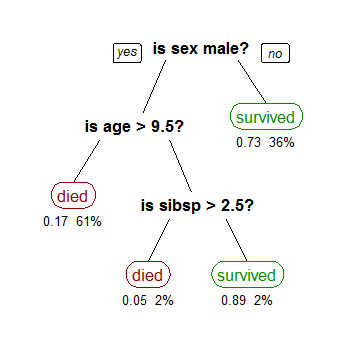
\includegraphics[scale=0.6]{img/decision_tree.png}
\caption{Drzewo decyzyjne dla problemu klasyfikacji losu pasażerów statku Titanic \cite{wikidecisiontree}}
\label{img:wiki_dec_tree}
\end{figure}

Dla złożonych zagadnień predykcji takich jak przewidywanie trendu giełdy, drzewa decyzyjne okazują się zbyt prostym modelem. Las losowy jest rozwinięciem koncepcji drzew decyzyjnych w zakresie metod zespołowych. Głównym założeniem jest stworzenie wielu drzew decyzyjnych i opieranie końcowego wyniku na podstawie poszczególnych wyników każdego z drzew. W celu wprowadzenia różnorodności podczas konstrukcji węzłów drzew, losowane są cechy spośród których będą dobrane cechy decyzyjne w danym węźle. Metoda ta zazwyczaj daje dużo lepsze efekty niż pojedyncze drzewa decyzyjne, oraz często pomaga w ograniczaniu zjawiska przeuczania (ang. overfitting).  

\subsection{Light GBM}

\textit{Light GBM} (Light Gradient Boosting Machine)\cite{lgbm} jest algorytmem z rodziny \textit{gradient boosting decision trees}. Algorytmy te oparte są o zespół drzew decyzyjnych. W przeciwieństwie do metody \textit{lasu losowego} konstrukcja kolejnych drzew jest wykonywana w sposób sekwencyjny, oraz zależny od wyników poprzednich drzew. Dzięki takiemu zabiegowi, zespół drzew dąży do ulepszenia swoich wyników jako całości. Algorytm \textit{light GBM} przewyższa inne algorytmy ze swojej klasy takie jak \textit{XGBoost} dzięki innemu podejściu do tworzenia drzew. Podczas gdy większość algorytmów powiększa drzewa decyzyjne wgłąb (\textit{level-wise}  rysunek \ref{img:level-wise}), \textit{light GBM} powiększa drzewa decyzyjne ze względu na liście (\textit{leaf-wise} rysunek \ref{img:leaf-wise}). Ten zabieg wraz z innymi optymalizacjami sprawia, że algorytm ten osiąga porównywalne wyniki do innych algorytmów ze swojej klasy, przy dużym skrócenia czasu uczenia się. 


\begin{figure}[H]%
\centering
\subfigure[Konstrukcja drzewa algorytmu \textit{light GBM}]{%
\label{img:level-wise}
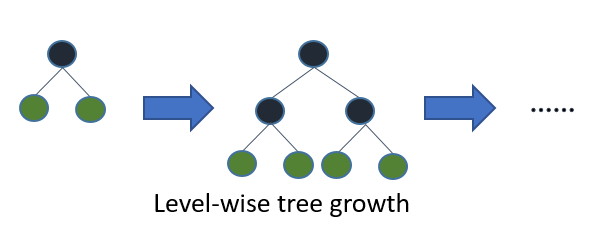
\includegraphics[scale=0.46]{img/lgbm-level-wise.png}}%
\qquad
\subfigure[Konstrukcja drzewa algorytmu \textit{light GBM}]{%
\label{img:leaf-wise}
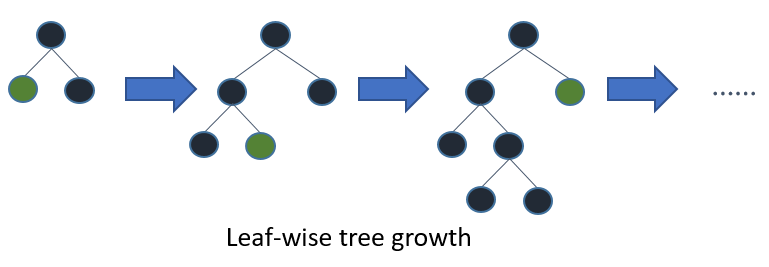
\includegraphics[scale=0.46]{img/lgbm-leaf-wise.png}}%
\caption{Porównanie konstrukcji drzew algorytmów z rodziny \textit{gradient boosting decision trees}}
\label{img:level-leaf-wise}
\end{figure}


\subsection{Wnioski i uwagi}

Predykcja kursu cen na giełdzie jest zagadnieniem zaawansowanym pod względem trudności i złożoności danych. Z tego powodu w tej pracy zastosowane zostały różnorodne modele klasyfikacyjne zgodne z najnowszymi trendami w dziedzinie uczenia maszynowego. Użycie zarówno tradycyjnych modeli sieci neuronowych jak i nowoczesnych technik takich jak algorytm \textit{Light GBM} pozwoliło na obszerne badanie w zakresie poszukiwania najlepszego klasyfikatora.

\newpage

\section{Eksperymenty numeryczne}

W poniższym rozdziale zostały opisane przeprowadzone eksperymenty numeryczne z wykorzystaniem różnych modeli predykcyjnych. Głównym celem tego rozdziału jest taki dobór modelu wraz z jego hiperparametrami, aby zmaksymalizować wybrane miary jakości. Podstawowym założeniem jest nauczanie modelu dla każdej ze spółek osobno (od zera), gdyż mogą one prezentować różną dynamikę i charakterystykę danych. Testy i optymalizacje były wykonyawne dla pojedynczej spółki \textit{GOOGL}, ze względu na ograniczenia mocy obliczeniowej i czasu. Końcowe porównywanie jakości różnych modeli zostało wykonane na podstawie wyników 10 spośród największych spółek z giełdy \textit{NASDAQ}. Wybrane spółki wraz z ich kapitalizacją rynkową zostały przedstawione w tabeli \ref{tab:biggest_companies}.


\begin{table}[H]
    \centering
    \begin{tabular}{|c|c|}
    \hline
        \textbf{Spółka} & \textbf{Kapitalizacja (mld USD)} \\ \hline
        MSFT & 1014.94 \\ \hline 
        AMZN & 920.5 \\ \hline 
        AAPL & 886.81 \\ \hline 
        GOOGL & 754.16 \\ \hline 
        FB & 517.6 \\ \hline 
        CSCO & 234.37 \\ \hline 
        PEP & 186.06 \\ \hline 
        INTC & 206.79 \\ \hline 
        AMGN & 107.4 \\ \hline 
        QCOM & 83.54 \\ \hline 
    \end{tabular}
    \caption{Spółki wykorzystane do oceny jakości nauczonych modeli}
    \label{tab:biggest_companies}
\end{table}

Wszystkie eksperymenty dla każdego zestawu parametrów zostały przeprowadzone 3 razy, a wartości dokładności i AUC zostały uśrednione. Czas uczenia jest czasem wykonania 3 iteracji testu dla danego zestawu parametrów. W rozdziale zawarto jedynie opis optymalizacji parametrów dających najciekawsze wyniki oraz te parametry, których zmiana przyniosła największą poprawę.

\bigskip

Parametrem rozpatrywanym z osobna przy każdym z modeli jest użycie metody \textit{PCA} do wstępnego przetworzenia danych. W tabeli \ref{tab:pca_component_number} przedstawiona została liczba zmiennych w zależności od wybranej wariancji przy reudukowaniu rozmiaru wektora wejściowego. Jak widać zmniejszenie wariancji o jedną tysięczną pozwala na ograniczenie rozmiaru wejściowych problemów o $\frac{1}{4}$, a zmniejszenie o jedną setną redukuje rozmiar aż o połowę. Nie można jednak z góry, bez testów, przesądzić jak ograniczanie rozmiaru zadania wpłynie na końcowe wyniki. 


\begin{table}[H]
    \centering
    \begin{tabular}{|c|c|}
    \hline
        \textbf{PCA (wariancja)} & \textbf{Liczba zmiennych} \\ \hline
        0.8000 & 4 \\ \hline 
        0.9000 & 8 \\ \hline 
        0.9500 & 12 \\ \hline 
        0.9700 & 16 \\ \hline 
        0.9800 & 18 \\ \hline 
        0.9900 & 23 \\ \hline
        0.9990 & 31 \\ \hline 
        0.9999 & 34 \\ \hline 
        Brak & 41 \\ \hline 
    \end{tabular}
    \caption{Wybrana wartość wariancji, a liczba zmiennych po wykonaniu PCA}
    \label{tab:pca_component_number}
\end{table}

\bigskip

Kolejnym parametrem rozpatrywanym przy każdym modelu jest \textbf{rozmiar zbioru testowego} w kontekście uczenia metodą kroczącą. Domyślnie modele były uczone w jednej iteracji metody kroczącej z wielkością zbioru testowego równej $0.2$ całego zbioru danych. Dzieląc zbiór testowy na mniejsze części, w każdej iteracji włączając już przetestowane próbki danych do zbioru treningowego, potencjalnie powiększany jest zbiór informacji przekazywanych modelom w trakcie uczenia. Taki zabieg jest powinien pozwolić na poprawę wyników i zbliżenie scenariusza testów do rzeczywistego wykorzystywania modelu predykcyjnego do handlu na giełdzie, gdzie model może być regularnie douczany wraz z upływem czasu. Poza maksymalnym rozmiarem zbioru testowego równego $0.2$ całego zbioru danych, wykorzystane zostały rozmiary $360, 180, 90, 45$ oraz $22$. Po każdym powiększeniu zbioru treningowego o nowe próbki modele były uczone od zera, a ich jakość była oceniana na podstawie kolejnej partii zbioru testowego.

\subsection{SVM}

Początkowo do testów SVM wykorzystane zostały domyślne parametry z biblioteki \textit{sklearn} \cite{bib:sklearnsvm}. Analizę optymalizacji maszyn wektorów nośnych należy zacząć od wyboru odpowiedniej funkcji jądra. Tabele \ref{tab:svm_kernel_binary} oraz \ref{tab:svm_kernel_discrete} przedstawiają wyniki klasyfikacji w zależności od wybranej funkcji jądra. W obu przypadkach klasyfikacji maszyny wektorów nośnych dają wyniki zbliżone do klasyfikacji metodą losową. W klasyfikacji binarnej najlepszy wynik uzyskała funkcja wielomianowa (ang. \textit{poly}). Jednak warto zauważyć iż dla tej funkcji metryka AUC jest bliska 0.5, podczas gdy SVM z funkcją rbf uzyskał AUC na poziomie 0.514.

\begin{table}[H]
    \centering
    \begin{tabular}{|c|c|c|c|}
    \hline
        \textbf{Funkcja jądra} & \textbf{Dokładność} & \textbf{AUC} & \textbf{Czas (s)} \\ \hline
linear  &  0.514132 &  0.500202 &    4.120035 \\ \hline
poly    &  \textbf{0.530283} &  0.501429 &    2.902045 \\ \hline
rbf     &  0.518170 &  \textbf{0.504402} &    3.482025 \\ \hline
sigmoid &  0.515478 &  0.504246 &    3.676025 \\ \hline
    \end{tabular}
    \caption{SVM: wyniki klasyfikacji binarnej w zależności od wykorzystanej funkcji jądrowej}
    \label{tab:svm_kernel_binary}
\end{table}

 Na rysunku \ref{img:svm_kernel_histograms_poly} przedstawiony został histogram predykcji dla funkcji wielomianowej, zaś na rysunku \ref{img:svm_kernel_histograms_rbf} histogram predykcji dla funkcji rbf. SVM z funkcją wielomianową osiąga lepszy wynik dokładności ponieważ w większości przypadków zwraca tę samą klasę. Taka obserwacja powtarza się za każdym razem gdy wynik miary AUC jest równy lub bliski 0.5. Z tego względu pomimo gorszej dokładności, funkcja \textit{rbf} okazała się lepsza.


\begin{figure}[H]%
\centering
\subfigure[Histogram predykcji dla jądra \textit{poly}]{%
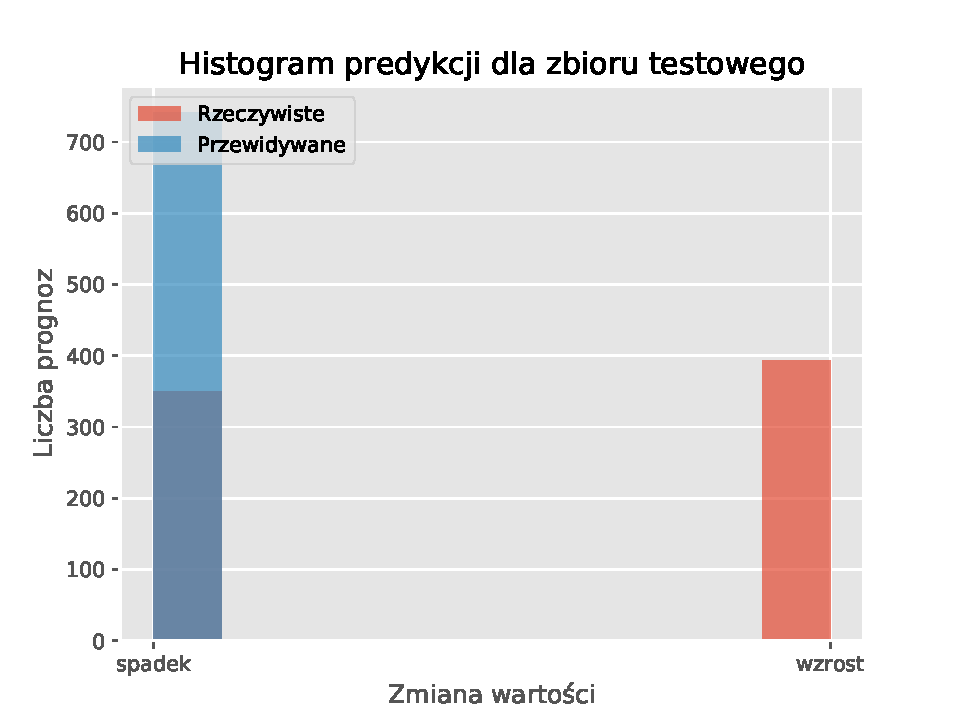
\includegraphics[scale=0.46]{img/svm_poly_hist.pdf}
\label{img:svm_kernel_histograms_poly}}%
\qquad
\subfigure[Histogram predykcji dla jądra \textit{rbf}]{%
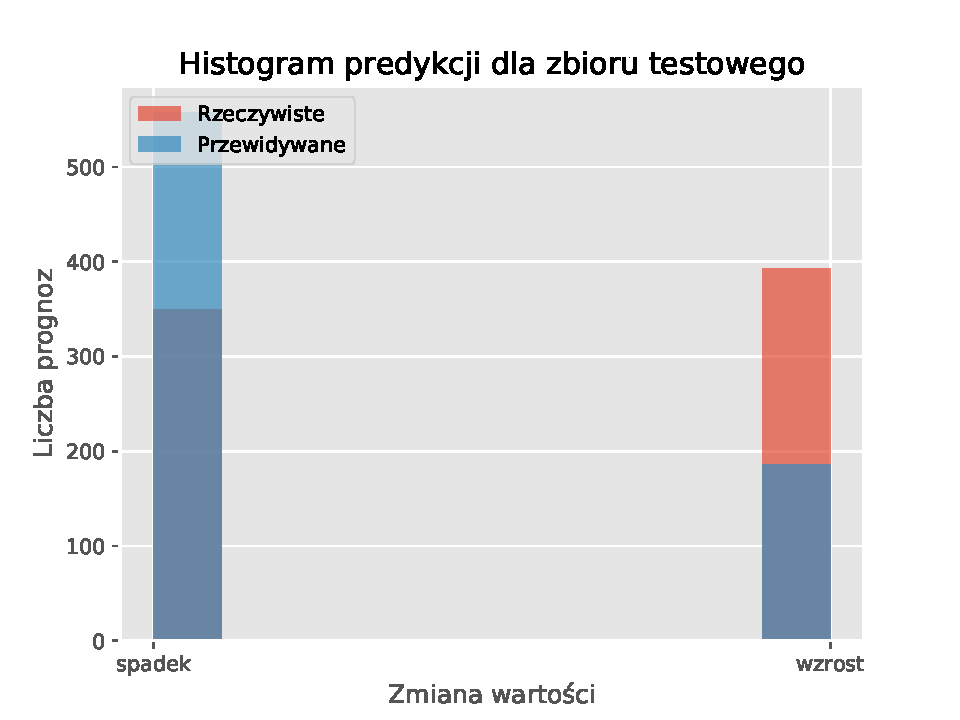
\includegraphics[scale=0.46]{img/svm_rbf_hist.pdf}
\label{img:svm_kernel_histograms_rbf}}%

\caption{Wykresy przedstawiające histogram predykcji dla poszczególnych klas w zależności od jądra (opracowanie własne)}
\label{img:svm_kernel_histograms}
\end{figure}

Dla klasyfikacji na 3 klasy najlepszy wynik dokładności daje \textit{liniowa} funkcja jądra, jednak lepsza względem miary AUC jest ponownie funkcja \textit{rbf}. W kolejnych testach dla obu klasyfikacji była wykorzystywana funkcja jądra \textit{rbf}.

\begin{table}[H]
    \centering
    \begin{tabular}{|c|c|c|c|}
    \hline
        \textbf{Funkcja jądra} & \textbf{Dokładność} & \textbf{AUC} & \textbf{Czas (s)} \\ \hline
linear  &  \textbf{0.383580} &  0.530851 &   10.743992 \\ \hline
poly    &  0.379542 &  0.517911 &    3.436018 \\ \hline
rbf     &  0.371467 &  \textbf{0.536517} &    4.302981 \\ \hline
sigmoid &  0.363392 &  0.518139 &    4.008035 \\ \hline
    \end{tabular}
    \caption{SVM: wyniki klasyfikacji na 3 klasy w zależności od wykorzystanej funkcji jądrowej}
    \label{tab:svm_kernel_discrete}
\end{table}


Kolejnym testem było porównanie wyników klasyfikacji w zależności od użycia metody PCA. W tabelach \ref{tab:svm_pca_binary} oraz \ref{tab:svm_pca_discrete} zostały przedstawione wyniki klasyfikacji w zależności od zachowanej wariancji danych przy użyciu metody PCA. Do klasyfikacji binarnej została wybrana wariancja $0.999$, zaś do klasyfikacji 3 klasy nie została użyta metoda PCA. W obu przypadkach różnice wynikające z użycia tej metody są marginalne.

\begin{table}[H]
    \centering
    \begin{tabular}{|c|c|c|c|}
    \hline
        \textbf{PCA} & \textbf{Dokładność} &  \textbf{AUC} &  \textbf{Czas (s)} \\ \hline
0.8                &  0.524899 &  0.497434 &    1.402048 \\ \hline
0.85               &  0.527591 &  0.496481 &    1.552432 \\ \hline
0.9                &  \textbf{0.534320} &  0.496668 &    1.660337 \\ \hline
0.95               &  0.518170 &  0.500580 &    2.294639 \\ \hline
0.97               &  0.519515 &  0.506320 &    2.853679 \\ \hline
0.98               &  0.520861 &  0.502179 &    3.790034 \\ \hline
0.99               &  0.514132 &  0.500845 &    2.595666 \\ \hline
0.999 				&  0.518170 &  \textbf{0.508287} &    2.823455 \\ \hline
0.9999             &  0.518170 &  0.499701 &    2.962357 \\ \hline
Brak                &  0.518170 &  0.501021 &    3.428985 \\ \hline
    \end{tabular}
    \caption{SVM: wyniki klasyfikacji binarnej w zależności od wybranej wartości wariancji w metodzie PCA}
    \label{tab:svm_pca_binary}
\end{table}

Dla klasyfikacji wieloklasowej widoczny jest proporcjonalny spadek miary AUC przy zmniejszaniu użytej wariancji w metodzie PCA. Wynika to ze zmniejszania liczby danych wejściowych, co zmniejsza ilość informacji przekazywanych do modelu.

\begin{table}[H]
    \centering
    \begin{tabular}{|c|c|c|c|}
    \hline
        \textbf{PCA} & \textbf{Dokładność} &  \textbf{AUC} &  \textbf{Czas (s)} \\ \hline
0.8                &  0.379542 &  0.514385 &    1.982013 \\ \hline
0.85               &  0.378197 &  0.524374 &    2.111366 \\ \hline
0.9                &  0.382234 &  0.522026 &    2.248027 \\ \hline
0.95               &  0.379542 &  0.526517 &    2.530379 \\ \hline
0.97               &  \textbf{0.383580} &  0.531114 &    2.652357 \\ \hline
0.98               &  0.379542 &  0.534494 &    2.765672 \\ \hline
0.99               &  0.378197 &  0.535341 &    2.966672 \\ \hline
0.999			   &  0.370121 &  0.535625 &    3.547385 \\ \hline
0.9999             &  0.371467 &  0.536259 &    4.062329 \\ \hline
Brak                &  0.371467 &  \textbf{0.537476} &    4.936680 \\ \hline
    \end{tabular}
    \caption{SVM: wyniki klasyfikacji na 3 klasy w zależności od wybranej wartości wariancji w metodzie PCA}
    \label{tab:svm_pca_discrete}
\end{table}


Następnym optymalizowanym parametrem był parametr kary \textit{C}. Wpływa on na wielkość marginesu separacji hiperpłaszczyzny od danych. Im większa wartość \textit{C} tym mniejszy margines. Domyślną wartością \textit{C} jest 1. Niestety manipulacja tym parametrem również nie pozwoliła na poprawę wyników (tabela \ref{tab:svm_c_binary} oraz \ref{tab:svm_c_discrete}). Najlepszą wartością \textit{C} dla klasyfikacji binarnej okazała się wartość domyślna 1, zaś dla klasyfikacji na 3 klasy wybrana została wartość 10. 


\begin{table}[H]
    \centering
    \begin{tabular}{|c|c|c|c|}
    \hline
        \textbf{C} & \textbf{Dokładność} & \textbf{AUC} & \textbf{Czas (s)} \\ \hline
0.005 &  0.528937 &  0.500000 &    2.808055 \\ \hline
0.01  &  0.528937 &  0.500685 &    2.804866 \\ \hline
0.1   &  \textbf{0.528937} &  0.500000 &    2.768114 \\ \hline
0.5   &  0.520861 &  0.500000 &    2.731033 \\ \hline
1.0   &  0.518170 &  \textbf{0.506115} &    2.789680 \\ \hline
5.0   &  0.497981 &  0.499756 &    2.813997 \\ \hline
10.0  &  0.493943 &  0.490091 &    2.746713 \\ \hline
25.0  &  0.487214 &  0.489592 &    3.164728 \\ \hline
50.0  &  0.492598 &  0.494963 &    3.536671 \\ \hline
100.0 &  0.502019 &  0.501905 &    4.065111 \\ \hline

    \end{tabular}
    \caption{SVM: wyniki klasyfikacji binarnej w zależności wykorzystanego parametru C}
    \label{tab:svm_c_binary}
\end{table}


\begin{table}[H]
    \centering
    \begin{tabular}{|c|c|c|c|}
    \hline
        \textbf{C} & \textbf{Dokładność} & \textbf{AUC} & \textbf{Czas (s)} \\ \hline
0.005 &  0.378197 &  0.530304 &    3.846018 \\ \hline
0.01  &  0.378197 &  0.533718 &    3.948358 \\ \hline
0.1   &  0.378197 &  0.531298 &    4.161030 \\ \hline
0.5   &  0.380888 &  0.534350 &    4.173678 \\ \hline
1.0   &  0.371467 &  0.536236 &    4.281026 \\ \hline
5.0   &  0.352624 &  0.536422 &    4.293353 \\ \hline
10.0  &  0.374159 &  \textbf{0.539444} &    4.433025 \\ \hline
25.0  &  \textbf{0.380888} &  0.538117 &    5.024735 \\ \hline
50.0  &  0.355316 &  0.536604 &    5.575662 \\ \hline
100.0 &  0.351279 &  0.536096 &    6.036690 \\ \hline
    \end{tabular}
    \caption{SVM: wyniki klasyfikacji na 3 klasy w zależności wykorzystanego parametru C}
    \label{tab:svm_c_discrete}
\end{table}


Na koniec wykonane zostały testy dokładności w zależności od rozmiaru zbioru testowego w kontekście uczenia SVM metodą kroczącą. Z wyników w tabelach \ref{tab:svm_walk_forward_binary} oraz \ref{tab:svm_walk_forward_discrete} można zauważyć iż ta optymalizacja dała najlepszą poprawę wyników. W przypadku użycia zbioru testowego o 360 próbkach dokładność klasyfikacji wzrosła aż o 4\%, a dla klasyfikacji wieloklasowej 2.5\%. Biorąc pod uwagę również miarę AUC dla klasyfikacji binarnej został wybrany zbiór testowy o 45 prókach, zaś dla klasyfikacji na 3 klasy wybrana została liczba 90 próbek.


\begin{table}[H]
    \centering
    \begin{tabular}{|c|c|c|c|}
    \hline
        \textbf{Rozmiar zbioru testowego} & \textbf{Dokładność} & \textbf{AUC} & \textbf{Czas (s)} \\ \hline
max                        &   0.518170 &  0.506115 &    2.789680 \\ \hline
360.0                         &  \textbf{0.558112} &  0.505209 &    9.710351 \\ \hline
180.0                         &  0.549219 &  0.502204 &   16.300354 \\ \hline
90.0                          &  0.529118 &  0.502368 &   27.596030 \\ \hline
45.0                          &  0.529412 &  \textbf{0.512139} &   51.312350 \\ \hline
22.0                          &  0.520310 &  0.507897 &  104.139698 \\ \hline

    \end{tabular}
    \caption{SVM: wyniki klasyfikacji binarnej w zależności od rozmiaru zbioru testowego}
    \label{tab:svm_walk_forward_binary}
\end{table}



\begin{table}[H]
    \centering
    \begin{tabular}{|c|c|c|c|}
    \hline
        \textbf{Rozmiar zbioru testowego} & \textbf{Dokładność} & \textbf{AUC} & \textbf{Czas (s)} \\ \hline
max                       &  0.374159 &  0.539444 &    4.433025 \\ \hline
360.0                         &  0.402264 &  0.535808 &   17.586026 \\ \hline
180.0                         &  \textbf{0.402834} &  0.550035 &   26.971038 \\ \hline
90.0                          &  0.385252 &  \textbf{0.550752} &   47.326667 \\ \hline
45.0                          &  0.377238 &  0.547582 &   89.569035 \\ \hline
22.0                          &  0.389424 &  0.546290 &  183.732708 \\ \hline
    \end{tabular}
    \caption{SVM: wyniki klasyfikacji na 3 klasy w zależności od rozmiaru zbioru testowego}
    \label{tab:svm_walk_forward_discrete}
\end{table}
    
W końcowych testach dla obu rodzajów klasyfikacji został użyty zbiór testowy o 360 próbkach.

\subsection{Sieci neuronowe}

Sieci neuronowe posiadają wiele parametrów, których zmiana może znacznie wpłynąć jakość klasyfikacji. Pierwszym analizowanym parametrem, był parametr wariancji przy redukcji rozmiaru problemu metodą PCA. Wyniki testów klasyfikacji binarnej dla różnych progów wariancji, zostały przedstawione w tabeli \ref{tab:nn_pca_binary}.  Najlepszy wynik $\sim 0.53$ AUC został uzyskany przy zachowaniu 0.999 wariancji zbioru danych wejściowych.

\begin{table}[H]
    \centering
    \begin{tabular}{|c|c|c|c|}
    \hline
        \textbf{PCA} & \textbf{Dokładność} &  \textbf{AUC} &  \textbf{Czas (s)} \\ \hline
0.8                &  0.531180 &  0.523126 &   49.905135 \\ \hline
0.85               &  0.523105 &  0.484570 &   40.372782 \\ \hline
0.9                &  0.533872 &  0.526000 &   41.801608 \\ \hline
0.95               &  0.528488 &  0.517909 &   43.106699 \\ \hline
0.97               &  \textbf{0.542844} &  0.525625 &   36.604079 \\ \hline
0.98               &  0.531180 &  0.513949 &   32.071058 \\ \hline
0.99               &  0.523105 &  0.508930 &   36.366585 \\ \hline
0.999              &  0.536563 &  \textbf{0.530908} &   40.616403 \\ \hline
0.9999             &  0.528488 &  0.511761 &   37.257610 \\ \hline
Brak               &  0.543742 &  0.524570 &   15.667901 \\ \hline

    \end{tabular}
    \caption{MLP: wyniki klasyfikacji binarnej w zależności od wybranej wartości wariancji}
    \label{tab:nn_pca_binary}
\end{table}

Takie same testy zostały przeprowadzone dla klasyfikacji na 3 klasy. Wyniki zostały zaprezentowane w tabeli \ref{tab:nn_pca_discrete}. Najlepsze wyniki zostały uzyskane wówczas gdy dane nie zostały przetworzone metodą PCA.

\begin{table}[H]
    \centering
    \begin{tabular}{|c|c|c|c|}
    \hline
        \textbf{PCA} & \textbf{Dokładność} &  \textbf{AUC} &  \textbf{Czas (s)} \\ \hline
0.8                &  0.380888 &  0.544181 &  113.261235 \\ \hline
0.85               &  0.372813 &  0.533684 &   96.453397 \\ \hline
0.9                &  0.381786 &  0.543038 &   94.264481 \\ \hline
0.95               &  0.371467 &  0.533985 &   98.159968 \\ \hline
0.97               &  0.375056 &  0.527683 &   90.220092 \\ \hline
0.98               &  0.369224 &  0.528660 &   75.099063 \\ \hline
0.99               &  0.384029 &  0.536447 &   67.764308 \\ \hline
0.999              &  0.385823 &  0.541818 &   72.476670 \\ \hline
0.9999             &  0.382683 &  0.545369 &   64.853820 \\ \hline
Brak                &  \textbf{0.392553} &  \textbf{0.548908} &   62.872527 \\ \hline
    \end{tabular}
    \caption{MLP: wyniki klasyfikacji na 3 klasy w zależności od wybranej wartości wariancji}
    \label{tab:nn_pca_discrete}
\end{table}

Przy następnych testach dla klasyfikacji binarnej została wykorzystana wartość wariancji $0.999$, zaś do klasyfikacji na 3 klasy dane nie były redukowane metodą PCA.

\bigskip

Następnym parametrem zbadanym podczas uczenia sieci jest liczba warstw ukrytych wraz z liczbą neuronów w każdej z warstw. Dla uproszczenia eksperymentów liczba warstw ukrytych w sieci neuronowej została ograniczona do wartości \{0, 1, 2\}, zaś liczba neuronów w każdej z warstw była taka sama. Wyniki mierzone miarą AUC dla klasyfikacji binarnej zostały przedstawione w tabeli \ref{tab:nn_layers_binary}. Dla tego rodzaju klasyfikacji najlepszym modelem okazał się model sieci neuronowej złożony z jednej z warstwy wejściowej, jednej warstwy ukrytej o 10 neuronach oraz warstwy wyjściowej. Uzyskał on wynik \textbf{0.532} AUC i $\sim 54\%$ dokładności.


Model bez warstwy ukrytej w przypadku klasyfikacji binarnej okazuje się najlepszy najprawdopodobniej ze względu na pojedynczy neuron w warstwie wyjściowej. Taka uproszczona architektura pozwala na znalezienie odpowiednich zależności w danych bez dodawania warstw ukrytych. Wyniki wydają się być odwrotnie proporcjonalne do liczby użytych neuronów, lecz nie odbiegają znacznie od najlepszego wyniku.

\begin{table}[H]
    \centering
    \begin{tabular}{|c|c|c|c|c|c|c|c|c|c|c|c|}
        \hline
         & &  \multicolumn{10}{c|}{Liczba neuronów w każdej warstwie}  \\ \hline
        \multirow{4}{*}{Warstwy} & & 0 & 2 & 3 & 4 & 5 & 6 & 7 & 8 & 9 & 10  \\ \cline{2 - 12}
			& 0 & 0.509 & - & - & - & - & - & - & - & - & - \\ \cline{2 - 12} 
			& 1 & - &  0.512 &  0.526 &  0.516 &  0.517 &  0.52 &  0.526 &  0.513 &  0.516  & \textbf{0.532} \\ \cline{2 - 12} 
			& 2 & - & 0.515 &    0.51 &   0.526 &   0.514 &    0.52 &     0.5 &   0.524 &   0.518 & 0.518 \\ \cline{2 - 12} \hline

    \end{tabular}
    \caption{MLP: wartości miary AUC dla różnych konfiguracji warstw ukrytych i liczby neuronów dla klasyfikacji binarnej (wyniki zaokrąglone)}
    \label{tab:nn_layers_binary}
\end{table}

Analogicznie do klasyfikacji binarnej został przeprowadzony test dla klasyfikacji na 3 klasy, wyniki przedstawiono w tabeli \ref{tab:nn_layers_discrete}. Najlepszy wynik \textbf{0.858} AUC ($\sim 68\%$ dokładności) został osiągnięty przy użyciu jednej warstwy ukrytej o 10 neuronach. W odróżnieniu do klasyfikacji binarnej, warstwa wyjściowa posiada 3 neurony, a co za tym idzie, potrzebna jest bardziej skomplikowana architektura sieci do uzyskania optymalnego wyniku. Zauważyć można również iż wykorzystanie wielu warstw ukrytych o małej liczbie neuronów znacznie pogarsza wynik co jest spowodowane zbyt małą liczbą połączeń między kolejnymi warstwami by zachować zależności między danymi.

\begin{table}[H]
    \centering
    \begin{tabular}{|c|c|c|c|c|c|c|c|c|c|c|c|}
        \hline
         & &  \multicolumn{10}{c|}{Liczba neuronów w każdej warstwie}  \\ \hline
        \multirow{4}{*}{Warstwy} & & 0 & 2 & 3 & 4 & 5 & 6 & 7 & 8 & 9 & 10  \\ \cline{2 - 12}
			& 0 & 0.549 & - & - & - & - & - & - & - & - & - \\ \cline{2 - 12} 
			& 1 & - & 0.534 &  0.551 &  0.536 &  0.537 &  0.538 &  0.541 &  0.551 &  \textbf{0.565} & 0.556 \\ \cline{2 - 12} 
			& 2 & - & 0.527 &   0.543 &   0.535 &   0.548 &   0.548 &   0.544 &   0.539 &   0.542 &   0.545  \\ \cline{2 - 12} \hline

    \end{tabular}
    \caption{MLP: wartości miary AUC dla różnych konfiguracji warstw ukrytych i liczby neuronów dla klasyfikacji na 3 klasy (wyniki zaokrąglone)}
    \label{tab:nn_layers_discrete}
\end{table}

W kolejnych testach do klasyfikacji binarnej nie zostały użyte warstwy ukrytne, zaś do klasyfikacji na 3 klasy była wykorzystywana jedna warstwa ukryta z 10 neuronami.

\bigskip

Kolejnym analizowanym parametrem był rozmiar zbioru testowego wykorzystywanego w każdej iteracji uczenia modelu metodą kroczącą. Tabela \ref{tab:nn_walk_forward_test_binary} przedstawia wyniki dla różnych rozmiarów zbioru testowego. Skonstruowanie modelu na nowo i ponowne nauczanie po 360 sesjach giełdy poprawiło początkowy wynik o $\sim 6\%$ jednak bez poprawy miary AUC. W kolejnych testach ucząc model od nowa co 180, 90, 45 przetestowanych próbek, otrzymywany był podobny wynik w kontekście dokładności jednak stopniowo rosła miara AUC. Najlepszy wynik dla klasyfikacji binarnej został osiągnięty przy 11 próbkach w zbiorze testowym. Dzięki tak prostemu zabiegowi dokładność modelu ulepszyła się aż o $\sim 15\%$. Niestety wraz ze zmniejszaniem zbioru testowego znacząco zwiększa się czas przeprowadzanego testu. Uniemożliwiło to przetestowanie zbiorów testowych o mniejszej liczbie próbek. W prawdziwych warunkach nie jest to jednak problemem, gdyż ponowne stworzenie modelu każdego dnia na podstawie zbioru treningowego powiększonego o jedną próbkę trwa jedynie około minuty na przeciętnym laptopie. Najprawdopodobniej im częstsze są aktualizacje zbioru testowego tym lepiej.

\begin{table}[H]
    \centering
    \begin{tabular}{|c|c|c|c|}
    \hline
        \textbf{Rozmiar zbioru testowego} & \textbf{Dokładność} &  \textbf{AUC} &  \textbf{Czas (s)} \\ \hline 
max                           &  0.545666 &  0.532053 &   35.540564 \\  \hline
360                         &  0.603811 &  0.526711 &    55.064094 \\  \hline
180                         &  0.599391 &  0.543832 &   117.292397 \\  \hline
90                         &  0.585974 &  0.550549 &   253.321093 \\  \hline
45                         &  0.618500 &  0.577297 &   679.401087 \\  \hline
22                          &  0.653227 &  0.594625 &  2481.258675 \\  \hline
11                          &  \textbf{0.694853} &  \textbf{0.617139} &  3332.849607 \\ \hline
    \end{tabular}
    \caption{MLP: wyniki klasyfikacji binarnej w zależności od rozmiaru zbioru testowego}
    \label{tab:nn_walk_forward_test_binary}
\end{table}

W tabeli \ref{tab:nn_walk_forward_test_discrete} przestawione zostały wyniki dla klasyfikacji na 3 klasy. Tutaj, analogicznie do prostszego zagadnienia klasyfikacji, widać znaczną poprawę wyników przy przeuczaniu modelu raz na miesiąc lub częściej. Wynik dokładności wzrósł aż o $\sim 18\%$ dla zbioru testowego o 11 próbkach. Jak widać dane wejściowe z kolejnych dni muszą być w pewnym stopniu unikalne jeżeli regularne dodawanie ich do zbioru treningowego tak istotnie poprawia wydajność modelu.

\begin{table}[H]
    \centering
    \begin{tabular}{|c|c|c|c|}
    \hline
        \textbf{Rozmiar zbioru testowego} & \textbf{Dokładność} &  \textbf{AUC} &  \textbf{Czas (s)} \\ \hline
max                           &  0.405497 &  0.565743 &   38.663478 \\ \hline
360                         &  0.473350 &  0.564853 &   53.011780 \\ \hline
180                         &  0.463864 &  0.574608 &   129.239635 \\ \hline
90                        &  0.468935 &  0.591316 &   286.016509 \\ \hline
45                          &  0.482523 &  0.586196 &   725.585042 \\ \hline
22                         &  0.520761 &  0.603951 &  2186.040966 \\ \hline
11                          &  \textbf{0.587010} &  \textbf{0.630126} &  4452.325083 \\ \hline

    \end{tabular}
    \caption{MLP: wyniki klasyfikacji na 3 klasy w zależności od rozmiaru zbioru testowego}
    \label{tab:nn_walk_forward_test_discrete}
\end{table}

Ostatecznie dla klasyfikacji binarnej oraz klasyfikacji trójklasowej zostały użyte zbiory testowe z 11 próbkami.

\subsection{Random forest}

Testy lasów losowych rozpoczęte zostały od analizy przetworzenia danych metodą PCA. Najlepsze wyniki klasyfikacji binarnej zostały uzyskane przy wybraniu wariancji o wartości $0.9999$, zaś dla klasyfikacji dyskretnej najlepszy wynik został osiągnięty przy użyciu wartości $0.99$. (tabele \ref{tab:rf_pca_binary} oraz \ref{tab:rf_pca_discrete}). W przypadku obu problemów domyślne wartości parametrów w zestawieniu z różnymi wartościami wariancji nie były wystarczające aby przekroczyć dokładność klasyfikatora wybierającego zawsze najliczniejszą klasę.

\begin{table}[H]
    \centering
    \begin{tabular}{|c|c|c|c|}
    \hline
        \textbf{PCA} & \textbf{Dokładność} & \textbf{AUC} & \textbf{Czas (s)} \\ \hline
0.8                &  0.509197 &  0.507391 &    0.761020 \\ \hline
0.85               &  0.501310 &  0.501343 &    0.968029 \\ \hline
0.9                &  0.507402 &  0.507414 &    0.997705 \\ \hline
0.95               &  0.505608 &  0.503373 &    0.947346 \\ \hline
0.97               &  0.499776 &  0.500465 &    1.110348 \\ \hline
0.98               &  0.505608 &  0.501081 &    1.115674 \\ \hline
0.99               &  0.505608 &  0.502540 &    1.109342 \\ \hline
0.999			   &  0.502916 &  0.500568 &    1.320368 \\ \hline
0.9999             &  \textbf{0.512337} &  \textbf{0.509109} &    1.317005 \\ \hline
Brak                &  0.487214 &  0.494583 &    1.646342 \\ \hline
    \end{tabular}
    \caption{Random forest: wyniki klasyfikacji binarnej w zależności od wybranej wartości wariancji w metodzie PCA}
    \label{tab:rf_pca_binary}
\end{table}
\begin{table}[H]
    \centering
    \begin{tabular}{|c|c|c|c|}
    \hline
        \textbf{PCA} & \textbf{Dokładność} & \textbf{AUC} & \textbf{Czas (s)} \\ \hline
0.8                &  0.366981 &  0.530468 &    0.785003 \\ \hline
0.85               &  0.362046 &  0.529749 &    0.972335 \\ \hline
0.9                &  0.359803 &  0.531703 &    1.020022 \\ \hline
0.95               &  0.356214 &  0.534884 &    1.139678 \\ \hline
0.97               &  0.363840 &  0.532332 &    1.161355 \\ \hline
0.98               &  0.360700 &  0.535334 &    1.268677 \\ \hline
0.99               &  \textbf{0.371467} &  \textbf{0.533416} &    1.220346 \\ \hline
0.999		       &  0.353970 &  0.528446 &    1.461351 \\ \hline
0.9999             &  0.344998 &  0.529919 &    1.463011 \\ \hline
Brak                &  0.340063 &  0.527937 &    1.730347 \\ \hline
    \end{tabular}
    \caption{Random forest: wyniki klasyfikacji na 3 klasy w zależności od wybranej wartości wariancji w metodzie PCA}
    \label{tab:rf_pca_discrete}
\end{table}

Podstawowym parametrem przy używaniu modelu lasu losowego jest dobór odpowiedniej liczby drzew, tworzących las. W poprzednim teście ten parametr miał wartość 100. Im więcej drzew zostaje użyte tym bardziej wydłuża się czas obliczeń, jednak zwiększa się liczba elementów biorących udział w predykcji co potencjalnie może polepszać wyniki klasyfikacji. Tabele \ref{tab:rf_estimators_binary} oraz \ref{tab:rf_estimators_discrete} przedstawiają wyniki klasyfikacji w zależności od liczby drzew w lesie. Niestety dobór większej liczby drzew tylko nieznacznie poprawia otrzymywane wyniki, jednocześnie znacznie wydłużając czas obliczeń. Dla obu typów klasyfikacji najlepszy wynik uzyskał las liczący 1000 drzew.

\begin{table}[H]
    \centering
    \begin{tabular}{|c|c|c|c|}
    \hline
        \textbf{Liczba drzew} & \textbf{Dokładność} & \textbf{AUC} & \textbf{Czas (s)} \\ \hline
25         &  0.489064 &  0.489766 &    4.097520 \\ \hline
50         &  0.510777 &  0.497981 &    7.935522 \\ \hline
300        &  0.526597 &  0.509428 &   46.976032 \\ \hline
100        &  0.519908 &  0.504696 &   15.782012 \\ \hline
200        &  0.516855 &  0.500553 &   31.111518 \\ \hline
500        &  0.530207 &  0.508128 &   79.370979 \\ \hline
1000       &  \textbf{0.536895} &  \textbf{0.513701} &  167.971013 \\ \hline
1500       &  0.530844 &  0.510723 &  235.584647 \\ \hline
2000       &  0.524128 &  0.503414 &  386.938110 \\ \hline
    \end{tabular}
    \caption{Random forest: wyniki klasyfikacji binarnej w zależności od liczby utworzonych drzew}
    \label{tab:rf_estimators_binary}
\end{table}

\begin{table}[H]
    \centering
    \begin{tabular}{|c|c|c|c|}
    \hline
        \textbf{Liczba drzew} & \textbf{Dokładność} & \textbf{AUC} & \textbf{Czas (s)} \\ \hline
25         &  0.375962 &  0.544072 &    4.654499 \\ \hline
50         &  0.351224 &  0.527772 &    8.893512 \\ \hline
100       &  0.388278 &  0.544457 &   17.790018 \\ \hline
200        &  0.385810 &  0.551537 &   38.911032 \\ \hline
300        &  0.385863 &  0.554436 &   52.376497 \\ \hline
500        &  0.384005 &  0.549873 &   95.120014 \\ \hline
1000       &  0.380289 &  \textbf{0.555435} &  209.299582 \\ \hline
1500       &  0.384536 &  0.552294 &  309.298568 \\ \hline
2000      &  \textbf{0.393720} &  0.550339 &  368.229640 \\ \hline
    \end{tabular}
    \caption{Random forest: wyniki klasyfikacji na 3 klasy w zależności od liczby utworzonych drzew}
    \label{tab:rf_estimators_discrete}
\end{table}

Ostatnim przeanalizowanym parametrem podobnie jak dla poprzednich modeli jest rozmiar zbioru testowego dla uczenia metodą kroczącą. W przeciwieństwie do modelu sieci neuronowych metoda lasu losowego nie wykazuje poprawy podczas iteracyjnej ewaluacji modelu (tabele \ref{tab:rf_walk_forward_binary} oraz \ref{tab:rf_walk_forward_discrete}). Dla klasyfikacji binarnej najlepsze wyniki są uzyskane przy jednokrotnym nauczeniu oraz ewaluacji modelu, co oznacza że lasy losowe nie są w stanie przyswoić nowych informacji ponad te zawarte w podstawowym zbiorze treningowym.

\begin{table}[H]
    \centering
    \begin{tabular}{|c|c|c|c|}
    \hline
        \textbf{Rozmiar zbioru testowego} & \textbf{Dokładność} & \textbf{AUC} & \textbf{Czas (s)} \\ \hline
max                         & \textbf{0.536895} &  \textbf{0.513701} &  167.971013 \\ \hline
360                         &  0.516033 &  0.508988 &    5.581545 \\ \hline
180                         &  0.528705 &  0.500111 &    9.069501 \\ \hline
90                          &  0.529092 &  0.512414 &   18.859000 \\ \hline
45                          &  0.519182 &  0.515216 &   35.510000 \\ \hline
22                          &  0.510982 &  0.507777 &   70.693982 \\ \hline

    \end{tabular}
    \caption{Random forest: wyniki klasyfikacji binarnej w zależności od rozmiaru zbioru testowego}
    \label{tab:rf_walk_forward_binary}
\end{table}

Dla problemu klasyfikacji wieloklasowej wynik poprawił się nieznacznie przy użyciu zbioru testowego o 180 próbkach, jednak taka poprawa może być związana z  niedeterminizmem nauczania lasów losowych.

\begin{table}[H]
    \centering
    \begin{tabular}{|c|c|c|c|}
    \hline
        \textbf{Rozmiar zbioru testowego} & \textbf{Dokładność} & \textbf{AUC} & \textbf{Czas (s)} \\ \hline
max                         &   0.380289 &  0.555435 &  209.299582 \\ \hline
360                         &  0.368983 &  0.530595 &    6.315498 \\ \hline
180                         &  \textbf{0.391857} &  \textbf{0.559301} &   10.532493 \\ \hline
90                          &  0.385810 &  0.553763 &   18.632999 \\ \hline
45                          &  0.382353 &  0.551812 &   34.919000 \\ \hline
22                          &  0.369377 &  0.545302 &   67.158500 \\ \hline
    \end{tabular}
    \caption{Random forest: wyniki klasyfikacji na 3 klasy w zależności od rozmiaru zbioru testowego}
    \label{tab:rf_walk_forward_discrete}
\end{table}

\subsection{Light GBM}

Podobnie jak w przypadku poprzednich modeli dla Light GBM analizowana była zależność jakości klasyfikacji od redukcji rozmiaru danych metodą PCA. Wyniki tej analizy zostały przedstawione w tabelach \ref{tab:lgbm_pca_binary} oraz \ref{tab:lgbm_pca_discrete}. Dla klasyfikacji binarnej najlepszy wynik został uzyskany przy wybraniu wartości wariancji $0.9999$, zaś dla klasyfikacji na 3 klasy wybrana została wartość $0.999$.	

\begin{table}[H]
    \centering
    \begin{tabular}{|c|c|c|c|}
    \hline
        \textbf{PCA} & \textbf{Dokładność} & \textbf{AUC} & \textbf{Czas (s)} \\ \hline
0.8                &  0.533666 &  0.496954 &    0.050999 \\ \hline
0.85               &  0.527591 &  0.481774 &    0.056999 \\ \hline
0.9                &  0.515478 &  0.507728 &    0.076001 \\ \hline
0.95               &  0.527591 &  0.475249 &    0.085999 \\ \hline
0.97               &  0.532974 &  0.522090 &    0.094999 \\ \hline
0.98               &  0.514132 &  0.526354 &    0.124001 \\ \hline
0.99               &  0.526245 &  0.522392 &    0.134996 \\ \hline
0.999			   &  0.518170 &  0.532937 &    0.174997 \\ \hline
0.9999             &  \textbf{0.534320} &  \textbf{0.534631} &    0.199997 \\ \hline
Brak                &  0.528937 &  0.479128 &    0.176996 \\ \hline
    \end{tabular}
    \caption{Light GBM: wyniki klasyfikacji binarnej w zależności od wybranej wartości wariancji w metodzie PCA}
    \label{tab:lgbm_pca_binary}
\end{table}

\begin{table}[H]
    \centering
    \begin{tabular}{|c|c|c|c|}
    \hline
        \textbf{PCA} & \textbf{Dokładność} & \textbf{AUC} & \textbf{Czas (s)} \\ \hline
0.8                &  0.358008 &  0.536740 &    3.360000 \\ \hline
0.85               &  0.351279 &  0.519820 &    3.989996 \\ \hline
0.9                &  0.348587 &  0.530616 &    4.280000 \\ \hline
0.95               &  0.339166 &  0.521876 &    4.782035 \\ \hline
0.97               &  0.341857 &  0.523877 &    5.265002 \\ \hline
0.98               &  0.351279 &  0.534347 &    5.498029 \\ \hline
0.99               &  0.343203 &  0.537076 &    5.899996 \\ \hline
0.999			   &  \textbf{0.360700} &   \textbf{0.537781} &    7.377026 \\ \hline
0.9999             &  0.351279 &  0.532163 &    7.542000 \\ \hline
Brak                &  0.348587 &  0.513556 &    7.982000 \\ \hline
    \end{tabular}
    \caption{Light GBM: wyniki klasyfikacji na 3 klasy w zależności od wybranej wartości wariancji w metodzie PCA}
    \label{tab:lgbm_pca_discrete}
\end{table}

Kolejnym parametrem, który został wykorzystany do optymalizacji modelu Light GBM jest procent cech wykorzystanych do utworzenia każdego z drzew. Na przykład jeżeli ustawimy ten parametr na $0.5$ każde drzewo będzie utworzone biorąc pod uwagę tylko połowę kolumn z wektora wejściowego. Cechy są wybierane losowo w momencie tworzenia kolejnego drzewa z lasu. Wyniki tego eksperymentu przedstawione są w tabelach \ref{tab:lgbm_feature_fraction_binary} oraz \ref{tab:lgbm_feature_fraction_discrete}. W przypadku obu klasyfikacji najbardziej korzystne wyniki daje 40\% całego wektora danych przy tworzeniu każdego z drzew. Zmiana tego parametru pozwoliła na poprawienie miary AUC w szczególności dla problemu klasyfikacji na 3 klasy.

\begin{table}[H]
    \centering
    \begin{tabular}{|c|c|c|c|}
    \hline
        \textbf{Procent cech (\%)} & \textbf{Dokładność} & \textbf{AUC} & \textbf{Czas (s)} \\ \hline
10              &  0.527591 &  0.516379 &    0.079981 \\
20              &  0.527591 &  0.453973 &    0.051998 \\
30              &  0.520861 &  0.492021 &    0.106998 \\
40              &  \textbf{0.532974} &  \textbf{0.524115} &    0.103000 \\
50              &  0.530283 &  0.489753 &    0.136001 \\
60              &  0.528937 &  0.506194 &    0.133999 \\
70              &  0.519515 &  0.466358 &    0.167000 \\
80              &  0.524899 &  0.485616 &    0.239999 \\
90              &  0.520861 &  0.509935 &    0.222998 \\
100              &  0.518170 &  0.522937 &    0.354000 \\ \hline
    \end{tabular}
    \caption{Light GBM: wyniki klasyfikacji binarnej w zależności od procenta cech wykorzystanych do tworzenia pojedynczego drzewa}
    \label{tab:lgbm_feature_fraction_binary}
\end{table}

\begin{table}[H]
    \centering
    \begin{tabular}{|c|c|c|c|}
    \hline
        \textbf{Procent cech (\%)} & \textbf{Dokładność} & \textbf{AUC} & \textbf{Czas (s)} \\ \hline
10              &  0.353970 &  0.524868 &    4.424998 \\
20              &  0.362046 &  0.530661 &    4.206039 \\
30              &  0.366083 &  0.537645 &    5.727013 \\
40              &  0.379542 &  \textbf{0.545501} &    6.142997 \\
50              &  0.367429 &  0.538036 &    6.631509 \\
60              &  \textbf{0.386272} &  0.533570 &    7.849054 \\
70              &  0.371467 &  0.544252 &    8.437996 \\
80              &  0.376851 &  0.531958 &   10.309524 \\
90             &  0.368775 &  0.538629 &   10.570999 \\
100              &  0.360700 &  0.537781 &    9.501997 \\ \hline
    \end{tabular}
    \caption{Light GBM: wyniki klasyfikacji na 3 klasy w zależności od procenta cech wykorzystanych do tworzenia pojedynczego drzewa}
    \label{tab:lgbm_feature_fraction_discrete}
\end{table}

Metoda Light GBM daje możliwość wyboru używanej metody \textit{boostingu}. Domyślnym algorytmem jest \textit{boosting} drzew decyzyjnych (\textit{gbdt}). W tabelach \ref{tab:lgbm_boosting_binary} oraz \ref{tab:lgbm_boosting_discrete} zostały przedstawione wyniki użycia różnych metod \textit{boostingu}. Jak widać dla klasyfikacji binarnej domyślny parametr \textit{gbdt} okazuje się najlepszym. Dla klasyfikacji wieloklasowej lepszy wynik daje metoda \textit{goss}, poprawiając wynik dokładności o $\sim 1\%$.

\begin{table}[H]
    \centering
    \begin{tabular}{|c|c|c|c|}
    \hline
        \textbf{Boosting} & \textbf{Dokładność} & \textbf{AUC} & \textbf{Czas (s)} \\ \hline
dart     &  0.493943 &  0.493348 &    2.089002 \\ \hline
gbdt     &  \textbf{0.532974} &  \textbf{0.524115} &    0.106003 \\ \hline
gbrt     &  \textbf{0.532974} &  \textbf{0.524115} &    0.116003 \\ \hline
goss     &  0.502264 &  0.513801 &    0.160999 \\ \hline
    \end{tabular}
    \caption{Light GBM: wyniki klasyfikacji binarnej w zależności od wybranego rodzaju boostingu}
    \label{tab:lgbm_boosting_binary}
\end{table}

\begin{table}[H]
    \centering
    \begin{tabular}{|c|c|c|c|}
    \hline
        \textbf{Boosting} & \textbf{Dokładność} & \textbf{AUC} & \textbf{Czas (s)} \\ \hline
dart     &  0.379542 &  0.536733 &    7.363997 \\ \hline
gbdt     &  0.370121 &  0.532499 &    0.469003 \\ \hline
gbrt     &  0.370121 &  0.532499 &    0.405001 \\ \hline
goss     &  \textbf{0.386083} &  \textbf{0.545501} &    0.642004 \\ \hline
    \end{tabular}
    \caption{Light GBM: wyniki klasyfikacji na 3 klasy w zależności od wybranego rodzaju boostingu}
    \label{tab:lgbm_boosting_discrete}
\end{table}

Następnym optymalizowanym parametrem była maksymalna liczba w każdym z drzew wygenerowanych przez algorytm. Domyślną wartością jest liczba 31 liści na drzewo. Wyniki tego eksperymentu zostały przedstawione w tabelach \ref{tab:lgbm_num_leaves_binary} oraz \ref{tab:lgbm_num_leaves_discrete}. Dla klasyfikacj binarnej należało zwiększyć liczbę liści do 100, zaś dla klasyfikacji na 3 klasy domyślną wartość trzeba było zmniejszyć do 20 liści na drzewo. 

\begin{table}[H]
    \centering
    \begin{tabular}{|c|c|c|c|}
    \hline
        \textbf{Liczba liści} & \textbf{Dokładność} & \textbf{AUC} & \textbf{Czas (s)} \\ \hline
5        &  0.528937 &  0.532366 &    0.047833 \\ \hline
10       &  0.527591 &  0.524326 &    0.072111 \\ \hline
20       &  0.532974 &  0.531425 &    0.074405 \\ \hline
30       &  \textbf{0.532974} &  0.521301 &    0.083468 \\ \hline
50       &  0.510094 &  0.511029 &    0.149726 \\ \hline
60       &  0.512786 &  0.511014 &    0.152193 \\ \hline
70       &  0.527591 &  0.513144 &    0.166835 \\ \hline
80       &  0.518170 &  0.524326 &    0.183499 \\ \hline
90       &  0.528937 &  0.530051 &    0.209766 \\ \hline
100      &  0.527591 &  \textbf{0.533090} &    0.195496 \\ \hline
    \end{tabular}
    \caption{Light GBM: wyniki klasyfikacji binarnej w zależności od maksymalnej liczby liści w pojedynczym drzewie}
    \label{tab:lgbm_num_leaves_binary}
\end{table}

\begin{table}[H]
    \centering
    \begin{tabular}{|c|c|c|c|}
    \hline
        \textbf{Liczba liści} & \textbf{Dokładność} & \textbf{AUC} & \textbf{Czas (s)} \\ \hline
5        &  0.367429 &  0.532798 &    0.199490 \\ \hline
10       &  0.370121 &  0.524657 &    0.264794 \\ \hline
20       &  \textbf{0.373121} &  \textbf{0.535442} &    0.441423 \\ \hline
30       &  0.356662 &  0.530182 &    0.449705 \\ \hline
50       &  0.353970 &  0.534866 &    0.503601 \\ \hline
60       &  0.364738 &  0.526885 &    0.374543 \\ \hline
70       &  0.367429 &  0.525644 &    0.407347 \\ \hline
80       &  0.371467 &  0.526985 &    0.448030 \\ \hline
90       &  0.345895 &  0.530006 &    0.642411 \\ \hline
100      &  0.364738 &  0.523292 &    0.482326 \\ \hline

    \end{tabular}
    \caption{Light GBM: wyniki klasyfikacji binarnej w zależności od maksymalnej liczby liści w pojedynczym drzewie}
    \label{tab:lgbm_num_leaves_discrete}
\end{table}

Ostatnim badanym parametrem jest rozmiar zbioru testowego wykorzystanego podczas uczenia metodą kroczącą. Wyniki badania zostały przedstawione w tabelach \ref{tab:lgbm_walk_forward_binary} oraz \ref{tab:lgbm_walk_forward_discrete}. Dla modelu Light GBM widać znaczną poprawę w klasyfikacji przy używaniu zbioru testowego o jak najmniejszej liczbie próbek. W przypadku tworzenia na nowo modelu po każdej sesji giełdowej, dla klasyfikacji binarnej ten model osiąga dokładność na poziomie $\sim 82.5\%$, zaś dla klasyfikacji na 3 klasy dokładność była na poziomie $\sim 63.3\%$. Dalsze zmniejszanie zbioru testowego pogarszało wyniki wbrew oczekiwaniom.

\begin{table}[H]
    \centering
    \begin{tabular}{|c|c|c|c|}
    \hline
        \textbf{Rozmiar zbioru testowego} & \textbf{Dokładność} & \textbf{AUC} & \textbf{Czas (s)} \\ \hline
max   						  & 0.535666 &  0.533299 &  0.406716 \\ \hline
360                         &  0.552885 &  0.535815 &    1.437676 \\ \hline
180                        &  0.566788 &  0.584807 &    2.990968 \\ \hline
90                         &  0.565748 &  0.576246 &    4.564312 \\ \hline
45                         &  0.572890 &  0.589065 &   11.184603 \\ \hline
22                          &  0.567098 &  0.608441 &   19.594985 \\ \hline
11                          &  0.587010 &  0.655322 &   36.808001 \\ \hline
5                           &  0.656376 &  0.735940 &   29.527999 \\ \hline
2                           &  0.732527 &  0.867772 &   80.699034 \\ \hline
1                           &  \textbf{0.825034} &  \textbf{0.959651} &  152.520538 \\ \hline

    \end{tabular}
    \caption{Light GBM: wyniki klasyfikacji binarnej w zależności od rozmiaru zbioru testowego}
    \label{tab:lgbm_walk_forward_binary}
\end{table}

\begin{table}[H]
    \centering
    \begin{tabular}{|c|c|c|c|}
    \hline
        \textbf{Rozmiar zbioru testowego} & \textbf{Dokładność} & \textbf{AUC} & \textbf{Czas (s)} \\ \hline
max   						 &  0.386272 &  0.545294 &    0.239276 \\ \hline
360                         &  0.402173 &  0.544229 &    0.992623 \\ \hline
180                         &  0.410171 &  0.561560 &    1.336995 \\ \hline
90                         &  0.410787 &  0.565290 &    2.079703 \\ \hline
45                          &  0.407928 &  0.570754 &    3.960998 \\ \hline
22                          &  0.406048 &  0.579615 &    8.925999 \\ \hline
11                          &  0.419118 &  0.603412 &   17.156001 \\ \hline
5                           &  0.465772 &  0.657281 &   46.353997 \\ \hline
2                           &  0.536290 &  0.713070 &  108.588001 \\ \hline
1                           &  \textbf{0.632690} &  \textbf{0.812767} &  218.438081 \\ \hline
    \end{tabular}
    \caption{Light GBM: wyniki klasyfikacji na 3 klasy w zależności od rozmiaru zbioru testowego}
    \label{tab:lgbm_walk_forward_discrete}
\end{table}

\subsection{Podsumowanie i wnioski}

Końcowe wyniki \textbf{klasyfikacji binarnej} dla każdego z klasyfikatorów zostały oparte o testy przeprowadzone na 10 spółkach. Wyniki dokładności dla każdej ze spółek zostały zawarte w tabeli \ref{tab:comparison_final_binary}. Dodatkowo podane zostały uśrednione wyniki dokładności i AUC dla każdego z modeli. 

%TODO rysunek z dwóch kryteriów średnia dokładność (oś x) + średnia AUC (oś y)

 \begin{table}[H]
    \centering
    \begin{tabular}{|c|c|c|c|c|}
    \hline
        \textbf{Spółka} & \textbf{SVM} &  \textbf{MLP}  &  \textbf{Random forest}  &  \textbf{Light GBM} \\ \hline
AAPL   &  0.530176 & 0.694728  & 0.517177 & \textbf{0.753717}\\ \hline
AMGN   &  0.509749 &  0.712868 & 0.506500 &  \textbf{0.829926} \\ \hline
AMZN   &  0.494893 & 0.712868 & 0.634609 & \textbf{0.817844} \\ \hline
CSCO   &  0.549675 &  0.705782 & 0.494429 &  \textbf{0.762082} \\ \hline
FB     &  0.519515 & 0.697206 & 0.556657 & \textbf{0.789773} \\ \hline
GOOGL  &  0.519515 &  0.741422 & 0.496635 & \textbf{0.793680} \\ \hline
INTC   &  0.537175 & 0.689059  & 0.470260 & \textbf{0.793680} \\ \hline
MSFT   &  0.546468 & 0.738379 & 0.475372 &  \textbf{0.851301}\\ \hline
PEP    &  0.528319 & 0.722222  & 0.495822 & \textbf{0.837361} \\ \hline
QCOM   &  0.522748 &  0.706916 & 0.512999 & \textbf{0.836431} \\ \hline \hline
\textbf{Średnia dokładność} &  0.525713 & 0.712145 & 0.501703 & \textbf{0.809715} \\  \hline  
\textbf{Średnia AUC} &  0.508806 & 0.651943 & 0.509316 & \textbf{0.951182} \\  \hline
    \end{tabular}
    \caption{Końcowe wyniki dokładności dla klasyfikacji binarnej różnych spółek}
    \label{tab:comparison_final_binary}
\end{table}   

Najlepszy średni wynik uzyskał model Light GBM ze średnią dokładnością $\sim 80.1\%$ oraz AUC $\sim 0.951$ . Drugi najlepszy wynik osiągnął model sieci neuronowej z  $\sim 71\%$ dokładności i $\sim 0.652$ AUC. Modele SVM oraz random forest osiągneły wyniki zbliżone do losowej predykcji.

\bigskip

Model Light GBM okazał się najlepszy dla wszystkich spółek. Należy jednak wziąć pod uwagę iż model sieci neuronowej był trenowany co 11 sesji giełdowych, podczas gdy model Light GBM był uczony na nowo po każdej sesji giełdowej. Wynikało to z ograniczeń technicznych. W powyższych eksperymentach zostało wykazane silne powiązanie pomiędzy powiększaniem zbioru treningowego o najnowsze próbki z danymi, a końcową jakością modelu. Wykonanie testów dla modelu Light GBM trenowanego co 11 sesji daje średni wynik $\sim 61.5\%$ dokładności oraz $\sim 0.669$ AUC. W związku z tym należy mieć na uwadze iż model sieci neuronowej ma jeszcze dużo potencjału na poprawę. Przy używaniu modelu sieci neuronowej w praktyce ograniczenia techniczne nie występują ze względu na krótki czas pojedynczego uczenia modelu.

\bigskip

Dla modelu random forest można zauważyć pewną anomalię dla spółki \textit{AMZN}. Wynik $\sim 63.5\%$ dokładności widocznie odstaje od pozostałych predykcji tego modelu. Na rysunku \ref{img:amzn_googl_adjusted_comparison} zostało przedstawione porównanie zmian ceny zamknięcia spółki \textit{AMZN} ze spółką \textit{GOOGL}, dla której został uzyskany wynik $\sim 49.7\%$ dokładności. Dla spółki \textit{AMZN} widać dynamiczny wzrost ceny począwszy od 2015 roku. Model lasu losowego prawdopodobnie jest w stanie dokładniej przewidywać spółki o dynamicznym wzroście.

\begin{figure}[H]
\centering 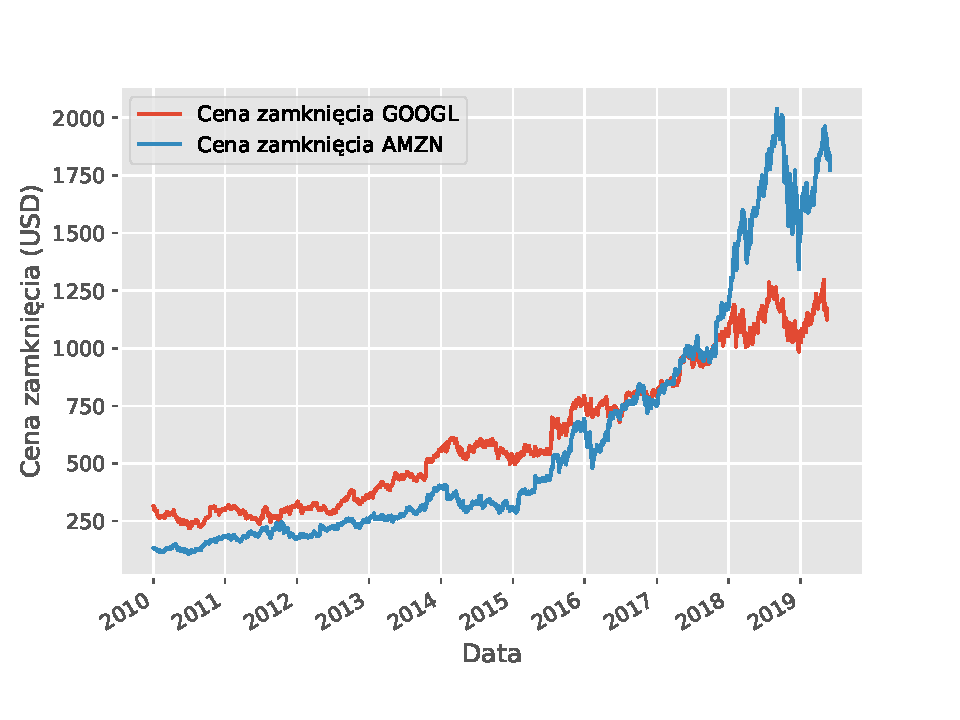
\includegraphics[scale=1]{img/AMZN_GOOGL_close_comparison.pdf}
\caption{Porównanie wykresów ceny zamknięcia spółek \textit{GOOGL} i \textit{AMZN} (opracowanie własne)}
\label{img:amzn_googl_adjusted_comparison}
\end{figure}

\bigskip

Dla \textbf{klasyfikacji na 3 klasy} zostały wykonane analogiczne testy dla 10 spółek. Wyniki zostały przedstawione w tabeli \ref{tab:comparison_final_discrete}. Podobnie jak dla poprzedniego problemu modele \textit{SVM} oraz \textit{random forest} nie wykazały dużo lepszej dokładności od losowego predyktora. Ponownie najlepszy okazał się model \textit{Light GBM} z dokładnością na poziomie $\sim 59.3\%$ oraz AUC $\sim 0.786$. Niewiele gorszy wynik dokładności osiągnął model sieci neuronowej $\sim 56.8\%$, jednak uzyskał on znacznie niższy wynik miary AUC $\sim 0.633$.

%TODO rysunek z dwóch kryteriów średnia dokładność (oś x) + średnia AUC (oś y)

\begin{table}[H]
    \centering
    \begin{tabular}{|c|c|c|c|c|}
    \hline
        \textbf{Spółka} & \textbf{SVM} &  \textbf{MLP}  &  \textbf{Random forest}  &  \textbf{Light GBM} \\ \hline
AAPL   &  0.354689 & 0.584751  & 0.358867 & \textbf{0.587361} \\ \hline
AMGN   &  0.369545 &  0.549268 & 0.352832 &  \textbf{0.553903} \\ \hline
AMZN   &  0.364903 & \textbf{0.568027} & 0.367224  & 0.562268 \\ \hline
CSCO   &  0.354689 &  0.569161 & 0.347261 &  \textbf{0.601301} \\ \hline
FB     &  0.382436 & 0.542850 & 0.371105 & \textbf{0.596591} \\ \hline
GOOGL  &  0.375505 &  0.564951 & 0.374159 & \textbf{0.616420} \\ \hline
INTC   &  0.354089 & 0.581633  & 0.345725 & \textbf{0.599442} \\ \hline
MSFT   &  0.358736 &   0.594671 & 0.351766 &  \textbf{0.635688} \\ \hline
PEP    &  0.390901 & 0.558107  & 0.340297 & \textbf{0.631970} \\ \hline
QCOM   &  0.378830 &  \textbf{0.558107} & 0.350511 & 0.546468 \\ \hline \hline
\textbf{Średnia dokładność} &  0.368432 & 0.567975 & 0.355975 & \textbf{0.593141} \\  \hline  
\textbf{Średnia AUC} &  0.549218 & 0.632774 & 0.538469 & \textbf{0.785912} \\  \hline
    \end{tabular}
    \caption{Końcowe wyniki dokładności dla klasyfikacji na 3 klasy różnych spółek}
    \label{tab:comparison_final_discrete}
\end{table}   

Pomimo gorszych warunków testu dla modelu sieci neuronowej (nowe próbki w zbiorze treningowym co 11 sesji giełdowych), uzyskał on lepszy wynik od modelu \textit{Light GBM} dla 2 spółek. Dodatkowo średnie wyniki tych dwóch modeli są dużo bardziej zbliżone. Dla klasyfikacji binarnej różnica w dokładności tych modeli wyniosła $\sim 9\%$, zaś dla klasyfikacji na 3 klasy różnica wyniosła jedynie $\sim 2.5\%$. 

\bigskip

Klasyfikacja wieloklasowa jest jednak zauważalnie cięższym zagadnieniem od klasyfikacji binarnej gdyż różnica w średnich wynikach dokładności wyniosła ponad $\sim 20\%$. Ta dysproporcja wydaje się być naturalna, ponieważ w przeciwieństwie do klasyfikacji binarnej podział na klasy nie wynika bezpośrednio z różnic cen na giełdzie. Trzecia klasa została wprowadzona w sposób sztuczny na podstawie progu opartego o marżę pobieraną od transakcji giełdowych, nie zaś na podstawie danych naturalnie występujących pośród danych giełdy. Takie działanie bez wątpienia powiększyło złożoność zagadnienia predykcji.

\bigskip

Dodatkowo dla problemu wieloklasowego przeprowadzona została analiza jakości klasyfikacji konkretnych klas. Na wykresie \ref{img:lgbm_roc_amzn} zostały przedstawione krzywe ROC dla 3 klas, wraz z ich mikro-średnią, dla modelu \textit{Light GBM}. Analizując wykres łatwo zauważyć dysproporcję pomiędzy AUC poszczególnych klas. Model dla tej spółki zaskakująco dobrze radzi sobie z predykcją klasy \textit{utrzymanie}. Wynik AUC dla tej klasy jest aż o $0.14$ większy od pozostałych klas. Taka postać rzeczy nie jest jednak regułą. Dla różnych spółek miary AUC dla poszczególnych klas mogą być bardzo zróżnicowane. Taka rozbieżność może być problematyczna na etapie używania nauczonego modelu do predykcji. Im większa rozbieżność między AUC poszczególnych klas tym gorzej. Może się bowiem okazać iż dwa modele o porównywalnej mierze AUC będą uzyskiwały rozbieżne wyniki w grze na giełdzie. Hipotetycznie dany model mógłby w ogóle nie przypisywać wejściowych próbek do jednej z klas, zaś pozostałe klasy estymować z wysokim prawdopodobieństwem. Na przykład model nie wskazujący nigdy klasy spadku, nie dawałby sygnału do sprzedaży akcji. To całkowicie wyklucza jego praktyczne użycie.

\begin{figure}[H]
\centering 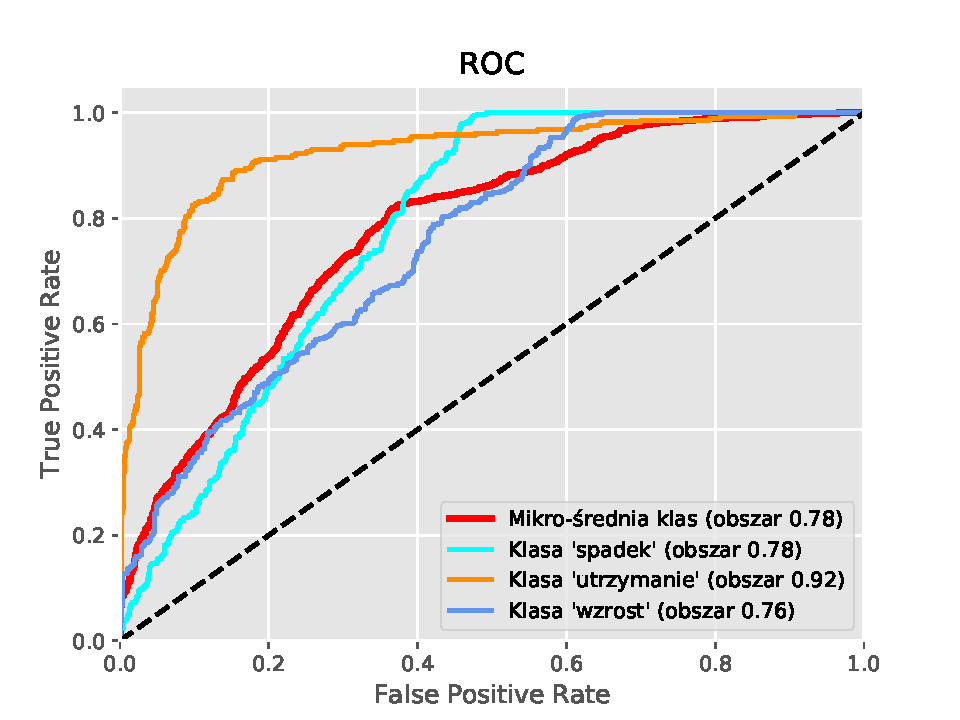
\includegraphics[scale=0.8]{img/AMZN_roc_lgbm.pdf}
\caption{Wykres ROC predykcji modelu \textit{Light GBM} dla klasyfikacji na 3 klasy spółki \textit{AMZN} (opracowanie własne)}
\label{img:lgbm_roc_amzn}
\end{figure}

\newpage

\section{Wspomaganie decyzji giełdowych}

Mając do wykorzystania klasyfikatory o wybranych parametrach można przystąpić do weryfikacji ich skuteczności na giełdzie. Ocena jakości odbyła się poprzez symulację uproszczonego modelu giełdy. Głównym założeniem było dokonywanie transakcji jedynie na początku sesji giełdowej tj. po cenie otwarcia. Taki scenariusz odzwierciedla wykonanie predykcji klasyfikayorem na podstawie danych z sesji giełdowej z dnia \textit{t} oraz podjęcie decyzji w najbliższym możliwym czasie tj. przy rozpoczęciu sesji w dniu \textit{t+1}. Jako zbiór treningowy dla każdej spółki wykorzystane zostały wszystkie dane od początku jej istnienia aż do 31 grudnia 2018. Symulacja giełdowa została przeprowadzona na danych od 1 stycznia 2019, aż do 6 lipca 2019. W tym okresie przeprowadzono 127 sesji giełdowych. Symulacja uwzględniała prowizję od każdej transakcji na poziomie 0.2\% jej wartości. Każda spółka była testowana osobno. Budżet dla każdej spółki wynosił \textit{100~000} dolarów.

\bigskip

Algorytm dokonujący transakcji opiera się na analizie kolejnych sesji giełdowych ze zbioru testowego. Jeżeli klasifikator przewiduje wzrost ceny, algorytm kupuje maksymalną możliwą liczbę akcji (musi to być liczba naturalna więc budżet nie zawsze jest całkowicie wykorzystany). Jeżeli algorytm jest w posiadaniu papierów wartościowych, a klasyfikator daje sygnał utrzymania ceny lub wzrostu, algorytm pozostaje bezczynny. Jeżeli algorytm jest w posiadaniu papierów wartościowych, a klasyfikator daje sygnał spadku ceny, algorytm wyprzedaje wszystkie posiadane akcje. Ostatnim krokiem algorytmu jest monetyzacja wszelkich zakupionych akcji w ostatniej sesji ze zbioru testowego w celu oszacowania zysków.

\bigskip

Do porównania uzyskanych wyników zastosowana była technika \textit{buy and hold}, która polega na kupieniu akcji odpowiednich spółek i pozostanie biernym na wahania rynku do czasu spieniężenia akcji.  Ta metoda jest preferowaną formą inwestowania analityków fundamentalnych, którzy często twierdzą iż niemożliwym jest wypracowanie ponadprzeciętnych zysków w oparciu o analizę techniczną i predykcję trendów. Innym wskaźnikiem stosowanym do oceny wyników aktywnego grania na giełdzie jest indeks giełdowy, który jest odwzorowaniem średniej zmiany wartości dla konkretnej grupy spółek. Inwestowanie w fundusze inwestycyjne oparte o indeksy giełdowe często jest uznawane za wygodną alternatywę do handlu na konkretnych akcjach, gdyż odzwierciedla szeroki rynek i nie wymaga dogłębnej analizy spółek.  Odpowiednim indeksem giełdowym do wybranych w tej pracy spółek jest \textit{S\&P 500} zawierającym 500 przedsiębiorstw o największej kapitalizacji notowanych na giełdach \textit{NYSE} oraz \textit{NASDAQ}. W okresie od 1 stycznia 2019 do 6 lipca 2019 indeks \textit{S\&P 500} zanotował wzrost o \textbf{18.45}\%.

\bigskip

Wyniki dla metody \textit{buy and hold} oraz klasyfikatorów binarnych zostały opisane w tabeli \ref{tab:comparison_simulation_binary}. Dzięki mniejszej liczbie próbek przy tej analizie model sieci neuronowych był uczony na nowo co dwie sesje giełdowe. Metoda \textit{buy and hold} pozwoliła na wypracowanie zysku na poziomie 124.41\% kapitału początkowego. Jak widać wyniki dla poszczególnych modeli są odzwierciedleniem porównania ich pod względem dokładności klasyfikacji (tabela \ref{tab:comparison_final_binary}). Najlepszy średni wynik na poziomie \textbf{140.01}\% kapitału początkowego uzsykał model sieci neuronowej, niewiele gorszy okazał się model \textit{Light GBM} z wynikiem około 131\%. Dla modelu SVM wynik 120\% jest odstępstwem od oczekiwań w porównaniu do dokładności tego modelu. Ta średnia wartość wydaje się być zawyżona przez wynik dla spółki \textit{QCOM}. Dla pozostałych spółek model SVM jest zauważalnie gorszy od biernego uczestnictwa w giełdzie. Najgorszy wynik około 107\% otrzymał model lasu losowego. Dla tego modelu również widać anomalię w przypadku spółki \textit{QCOM}. Analiza wykresu ceny zamknięcia tej spółki (rysunek \ref{img:qcom_adj_close}) pozwala dostrzec gwałtowne wahanie ceny w połowie kwietnia 2019. Przy takich dynamicznych zmianach nawet modele losowe mogą przypadkowo uzyskać wysoki zysk przy odpowiednich decyzjach. Na dłuższą metę takie anomalie są jednak amortyzowane, a modele z niską dokładnością dają dużo gorsze wyniki.

%TODO rysunek z dwóch kryteriów średni zysk (oś x) + średnia dokładność (oś y)


 \begin{table}[H]
    \centering
    \begin{tabular}{|c|c|c|c|c|c|}
    \hline
        \textbf{Spółka}  & \textbf{Buy and hold} & \textbf{SVM} &  \textbf{MLP}  &  \textbf{Random forest}  &  \textbf{Light GBM} \\ \hline
AAPL & 140.61 & 134.64  &  \textbf{143.02} & 100.23 & 137.64\\ \hline
AMGN & 97.23 &  91.93 & \textbf{121.91}  & 80.65 &  108.10 \\ \hline
AMZN & 126.58 &  120.51 & \textbf{145.56} & 113.13 & 129.36 \\ \hline
CSCO & 131.31 & 130.74  & 136.77  & 106.17 &  \textbf{139.56} \\ \hline
FB   & 143.52 & 142.41  & \textbf{179.30} & 125.21 & 156.43 \\ \hline
GOOGL & 105.97 &  94.58 &  \textbf{136.29} & 103.45 & 132.08 \\ \hline
INTC & 103.98 & 102.05  & 115.59  & 86.82 & \textbf{119.19} \\ \hline
MSFT &  136.12 & 111.70  &  133.97  & 108.04 & \textbf{140.00} \\ \hline
PEP  & 121.60 &  114.14 &  \textbf{122.26} & 94.63 & 119.30 \\ \hline
QCOM & 137.18 &  158.54 &  \textbf{165.43} & 157.12 & 135.70  \\ \hline \hline
\textbf{Średni zysk} & 124.41 & 120.12 & \textbf{140.01} &  107.55 & 131.74 \\  \hline 
\textbf{Średnia dokładność} &  - & 55.4\% & \textbf{84.2\%} &  52.8\% & 79.4\% \\  \hline   
    \end{tabular}
    \caption{Uzyskany zysk wyrażony w procentach początkowego budżetu (100 oznacza budżet wejściowy), wyniki symulacji dla klasyfikacji binarnej.}
    \label{tab:comparison_simulation_binary}
\end{table}   

Model sieci neuronowej oraz model \textit{Light GBM} uzyskały dużo lepsze wyniki od strategii \textit{buy and hold} (124\%) czy też indeksu giełdowego (118\%). Model sieci neuronowej nie uzyskał najlepszych wyników dla wszystkich spółek, jednak różnica na korzyść modelu \textit{Light GBM} nie była znaczna, a końcowy wynik dla sieci neuronowej jest aż o $\sim 8\%$ lepszy. Największą korzyść z wykorzystywania klasyfikatorów do handlu na giełdzie widać przy spółkach, które uzyskały najgorsze wyniki przy strategii \textit{buy and hold}. Dla spółki \textit{AMGN} odniesiona została strata na poziomie 3\% kapitału, jednak wykorzystanie modelu sieci neuronowej pozwala na ograniczenie ryzyka i wypracowanie zadowalającego zysku. Wynika to z faktu, iż główną zaletą aktywnego handlu na giełdzie jest spieniężanie akcji przed spadkiem ceny. Jeżeli dla danej spółki cena w głównej mierze rośnie, aktywne zarządzanie portfelem inwestycyjnym nie będzie w stanie znacznie poprawić zysku wynikającego z biernego posiadania akcji.

\begin{figure}[H]
\centering 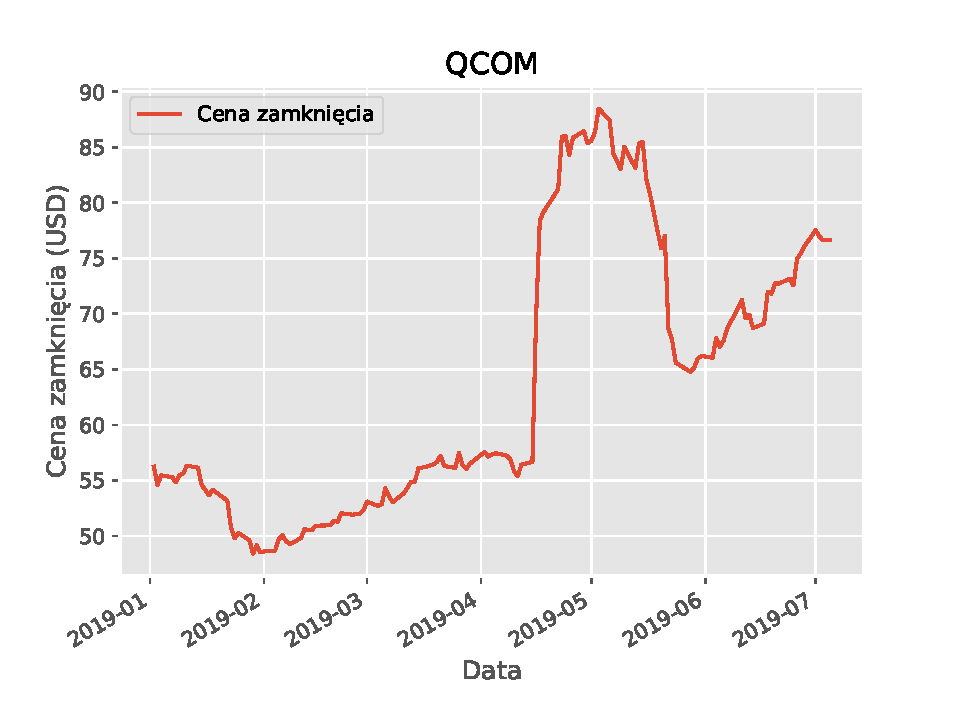
\includegraphics[scale=1]{img/QCOM_adj_close.pdf}
\caption{Wykres ceny zamknięcia spółki \textit{QCOM} (opracowanie własne)}
\label{img:qcom_adj_close}
\end{figure}


Analogiczne wyniki dla klasyfikatorów wieloklasowych zostały opisane w tabeli \ref{tab:comparison_simulation_discrete}. Podobnie jak w poprzednim teście zgodnie z oczekiwaniami najgorsze wyniki zostały uzyskane przez modele o najgorszej dokładności. Porównując model \textit{SVM} oraz \textit{random forest} zauważalny jest proporcjonalny wzrost zysku do wzrostu dokładności. Dla modelu \textit{Light GBM} uzyskany zysk jest niewiele gorszy do zysku tego modelu wykorzystującego klasyfikację binarną. Różnica kapitału końcowego wynosi jedynie $\sim 3.5\%$ podczas gdy różnica dokładności jest na poziomie $\sim 21\%$. Najlepszy wynik został uzsykany dla modelu sieci neuronowej, która wykazała wzrost kapitału do 138.03 \% co jest jedynie o $\sim 2\%$ gorszym wynikiem względem algorytmu opartego o klasyfikację binarną.

%TODO rysunek z dwóch kryteriów średni zysk (oś x) + średnia dokładność (oś y)


 \begin{table}[H]
    \centering
    \begin{tabular}{|c|c|c|c|c|c|}
    \hline
        \textbf{Spółka}  & \textbf{Buy and hold} & \textbf{SVM} &  \textbf{MLP}  &  \textbf{Random forest}  &  \textbf{Light GBM} \\ \hline
AAPL & 140.61 & 121.30  & \textbf{145.69}  & 111.01 & 145.94 \\ \hline
AMGN & 97.23 & 99.48  & \textbf{140.57} & 85.47 &  103.97 \\ \hline
AMZN & 126.58 &  109.94 & \textbf{136.23} & 117.90 & 127.84 \\ \hline
CSCO & 131.31 & 111.07  & \textbf{137.37}  & 101.92 & 122.74  \\ \hline
FB   & 143.52 &  128.23 & \textbf{152.81} & 124.79 & 151.15 \\ \hline
GOOGL & 105.97 &  94.98 &  \textbf{123.36} & 92.11 & 110.52 \\ \hline
INTC & 103.98 & 90.43  & \textbf{111.78}  & 83.59 & \textbf{111.78} \\ \hline
MSFT &  136.12 & 121.94  &  135.68  & 122.13 & \textbf{136.33} \\ \hline
PEP  & 121.60 &  121.13 & \textbf{126.09} & 117.00 & 119.90 \\ \hline
QCOM & 137.18 &  123.95 &  \textbf{170.69} & 95.67 & 151.21 \\ \hline \hline
\textbf{Średni zysk} & 124.41 & 112.24 & 138.03 & 105.16 & 128.14 \\  \hline  
\textbf{Średnia dokładność} &  - & 42.4\% & 75.1\% &  36.4\% & 58.2\% \\  \hline  
    \end{tabular}
    \caption{Uzyskany zysk wyrażony w procentach początkowego budżetu (100 oznacza budżet wejściowy), wyniki symulacji dla klasyfikacji na 3 klasy.}
    \label{tab:comparison_simulation_discrete}
\end{table}   

W symulacjach handlu na giełdzie z pomocą klasyfikatorów widoczna jest zależność końcowych wyników od wyników dokładności. Model sieci neuronowej oraz model \textit{Light GBM} uzyskały zadowalające wyniki dokładności i znacznie przewyższyły zysk z biernej inwestycji w wybrane akcje dla każdej z testowanych spółek. Model SVM oraz model lasu losowego nie potrafiły skutecznie przewidywać trendów giełdowych, a co za tym idzie uzyskały dużo gorsze wyniki od strategii \textit{buy and hold}. Dla przeprowadzonych testów, rozszerzenie problemu predykcji trendu o dodatkową trzecią klasę znacznie zwiększyło złożoność problemu, co można stwierdzić na podstawie uzyskanych wyników dokładności. Pomimo tego modele klasyfikujące na 3 klasy wykazywały zyski zbliżone do modeli klasyfikujących binarnie.

\bigskip


Analizę symulacji można pogłębić o wgląd w decyzje algorytmu. Rysunek \ref{img:amgn_wallet_buy_sell} przedstawia decyzje dokonywane przez algorytm używający klasyfikatora binarnego w zestawieniu z rzeczywistą ceną zamknięcia z każdego dnia. Na czerwono oznaczone są okresy gdy klasyfikator przewidywał spadek lub utrzymanie ceny, a w portfelu znajdowała się gotówka. Na zielono oznaczone zostały okresy gdy klasyfikator przewidywał wzrost lub utrzymanie ceny, a w portfelu znajdowały się akcje spółki \textit{AMGN}. Łatwo dostrzec, że klasyfikator ma największą dokładność w momentach gwałtownych spadków lub wzrostów ceny. W przypadku delikatnych zmian, algorytm zazwyczaj nie zmienia strategii co jest pożądanym zachowaniem pozwalającym na uniknięcie częstych opłat transakcyjnych dla domu maklerskiego. Model nie jest jednak perfekcyjny i nie zawsze jest w stanie odpowiednio przewidzieć zmiany ceny. Widać to w szczególności w okresie końca maja 2019, gdy nastąpił znaczny spadku ceny, zaś model nie dał sygnału do sprzedaży akcji co spowodowało utratę części kapitału.

\begin{figure}[H]
\centering 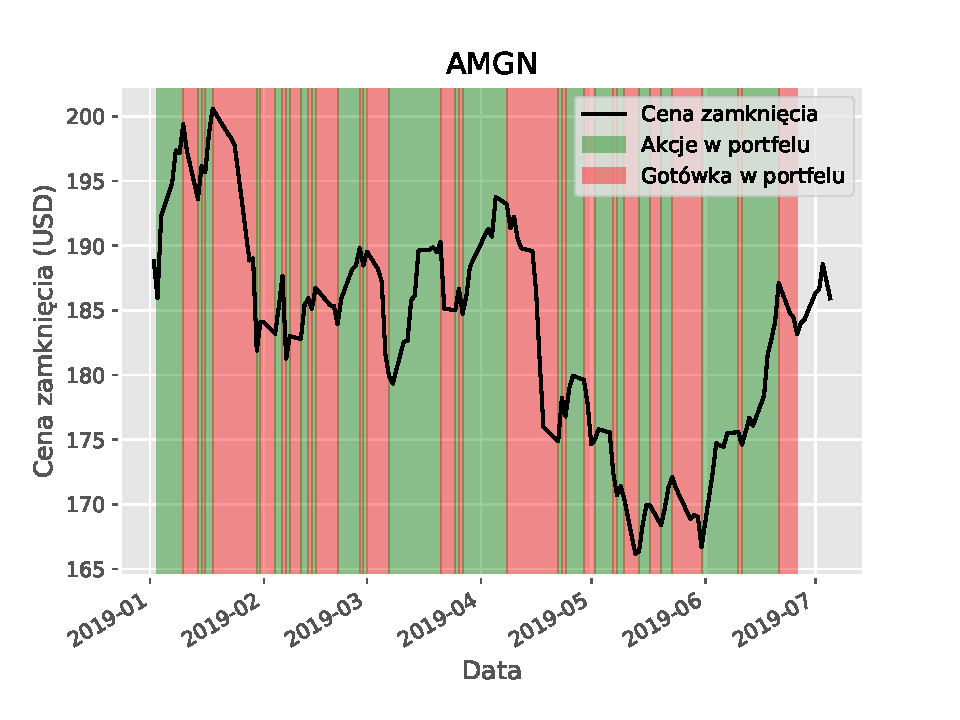
\includegraphics[scale=1.1]{img/AMGN-buy_and_sell_plot.pdf}
\caption{Wykres ceny akcji spółki \textit{AMGN} w zestawieniu z portfelem zarządzany przez algorytm używający wieloklasowego klasyfikatora MLP (opracowanie własne)}
\label{img:amgn_wallet_buy_sell}
\end{figure}

%TODO referencja bez odniesienia 


Na rysunku \ref{img:amgn_wallet_value} została przedstawiona wartość portfela algorytmu w zestawieniu z wartością portfela biernej inwestycji. To zestawienie pokazuje wyższość poprawnej predykcji nad biernym udziałem w giełdzie. Podczas gdy giełda odnotowuje spadki klasyfikator spienięża akcje zachowując środki, zaś gdy ceny akcji rosną algorytm poprawnie inwestuje zarabiając na wzroście ceny. W wykresach wartości obu portfeli widać znaczne podobieństwo jednak straty dla portfela zarządzanego przez algorytm z klasyfikatorem są znacznie mniejsze. Pozwala to reinwestować większość kapitału i z czasem różnica pomiędzy wartością obu portfeli coraz bardziej rośnie.

\begin{figure}[H]
\centering 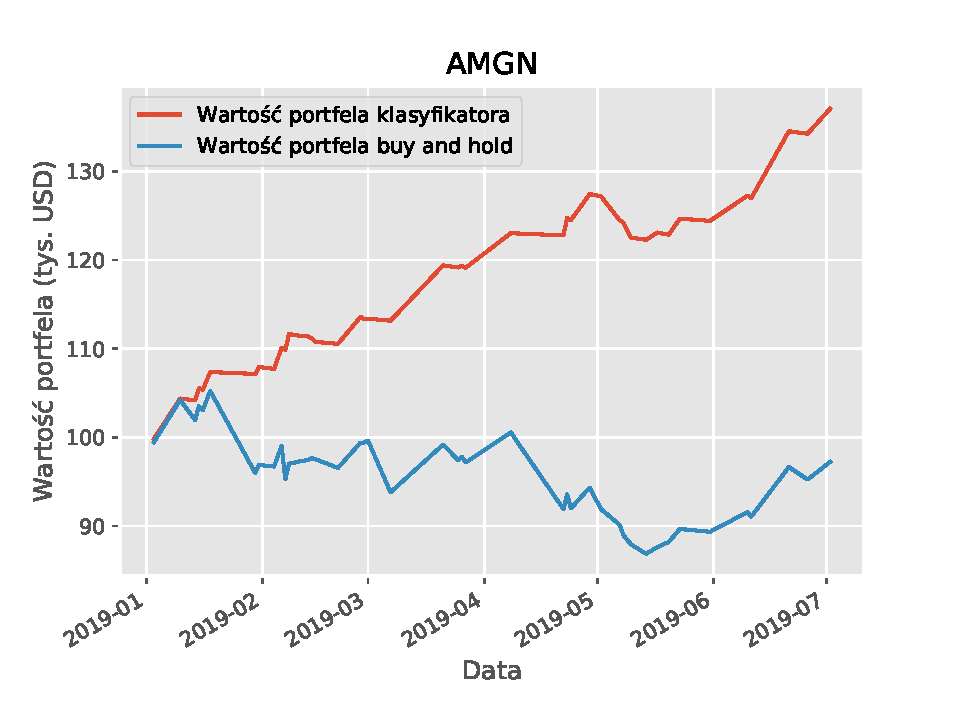
\includegraphics[scale=0.9]{img/AMGN-balance-plot.pdf}
\caption{Wykres wartości portfela algorytmu handlującego akcjami spółki \textit{AMGN} używającego wieloklasowego klasyfikatora MLP (opracowanie własne)}
\label{img:amgn_wallet_value}
\end{figure}

Warto dogłębniej zastanowić się nad użytecznością klasyfikacji na 3 klasy. Co prawda średni zysk dla handlu na podstawie klasyfikacji binarnej był o kilka punktów procentowych wyższy, jednak wprowadzenie trzeciej klasy do podstawowego problemu niesie za sobą inną korzyść. W tabeli \ref{tab:simulation_avg_value_vs_transactions} przedstawione został średni zysk dla najlepszych modeli oraz średnia liczba wykonanych transakcji podczas symulacji giełdowej.


%TODO też wykresik z punktami

 \begin{table}[H]
    \centering
    \begin{tabular}{|c|c|c|}
    \hline
        \textbf{Model}  & \textbf{Średni zysk} & \textbf{Średnia liczba transakcji}\\ \hline
            MLP binarny & 140.01 & 51.0 \\ \hline
            Light GBM binarny & 131.74 & 44.7 \\ \hline 
            \textbf{Średnia modeli binarnych} & \textbf{135.9} & \textbf{47.8} \\ \hline \hline
            
            MLP wieloklasowy & 138.03 & 39.2 \\ \hline
            Light GBM wieloklasowy & 128.14 & 23.3 \\ \hline
            \textbf{Średnia modeli wieloklasowych} & \textbf{133.1} & \textbf{31.2} \\ \hline
    \end{tabular}
    \caption{Porównanie średniego zysku z aktywnością danego modelu na giełdzie}
    \label{tab:simulation_avg_value_vs_transactions}
\end{table} 

 Modele klasyfikujące na 3 klasy wykonały średnio o 16 transakcji mniej niż klasyfikatory binarne (miesięcznie jest to średnio aż o 2.6 transakcji mniej). Wynika to z dodatkowej klasy, która pozwala na pozostanie biernym danego dnia giełdowego. Ta różnica w liczbie transakcji jest bardzo istotna w przypadku gdyby prowizje od każdej z transakcji były wyższe od założonej wartości 0.2\%. Przyjęta wartość jest jedną z najniższych prowizji na polskim rynku. Wyższe prowizje występują w szczególności gdy transakcje nie przekraczają jakiejś określonej kwoty (zazwyczaj jest to kilka tysięcy dolarów). W takim przypadku mniejsza liczba transakcji w dużo większym stopniu wpływa na końcowy wynik, a modele klasyfikacji na 3 klasy wykorzystują swój potencjał i okazują się lepsze od klasyfikatorów binarnych. Pomimo że różnica uzyskiwana przy omijaniu opłat transakcyjnych wydaje się być niewielka, na dłuższą metę, dzięki ponownemu inwestowaniu zyskaego kapitału, będzie ona rosła wykładniczo. W ekonomii to zjawisko nosi miano procenta składanego.
 
\newpage 
 
\section{Podsumowanie}

W pracy przedstawione zostały różnorodne dane mogące posłużyć do analiz cen giełdowych, oraz różne podejścia do problemu przewidywania zmian cen akcji na giełdzie. Wykonane eksperymenty klasyfikacji demonstrują możliwości predykcji zmian cen na giełdzie jedynie z wykorzystaniem podstawowych danych giełdowych oraz wskaźników analizy technicznej. Oba przedstawione problemy klasyfikacji uzyskały nad wyraz satysfakcjonujące wyniki przy użyciu różnorodnych metod uczenia maszynowego. Najlepsze wyniki uzyskał model sieci neuronowej oraz model maszyny wektorów nośnych.

\bigskip

Symulacje z użyciem algorytmu opartego o nauczone klasyfikatory dały doskonałe wyniki w grze na giełdzie. W większości przypadków uzyskiwany zysk znacznie przekroczył wzrost indeksu \textit{S\&P 500} oraz strategię \textit{buy and hold}. Takie rezultaty analiz daje podstawę do rozważenia użycia wbranych modeli w handlu na prawdziwym rynku papierów wartościowych. Jednakowoż wyniki symulacji użycia klasyfikatorów w handlu, pomimo bardzo obiecujących wyników, oparte zostały o uproszczony model giełdy. Przy prawdziwych transakcjach trzeba brać pod uwagę \textit{spread} ceny czyli różnicę między ceną kupna, a ceną sprzedaży danej akcji. Handlując dużą liczbą akcji, istotną rolę odgrywa podaż i popyt. Fakt iż algorytm w danym momencie sugeruje sprzedaż jakiejś liczby akcji po danej cenie, nie oznacza że znajdzie się na nie kupiec. Co za tym idzie cena sprzedaży może zostać obniżona przez konkurencyjną ofertę. Należy mieć na uwadze do jakiego stopnia opłaca się obniżać cenę przy zamiarze sprzedaży akcji oraz analogicznie wyznaczyć maksymalną cenę za jaką jesteśmy w stanie kupić akcje.  Dodatkowo w Polsce przy zyskach z gry na giełdzie trzeba pamiętać o podatku od dochodów kapitałowych (potocznie nazywany podatkiem Belki). Ze względu na symplifikację w kodzie źródłowym, wszystkie operacje zostały oparte o typy zmiennoprzecinkowe co oznacza utratę precyzji przy wykorzystywaniu ułamków, z tego powodu wszelkie wyniki w tej pracy należy traktować jako zaokrąglenia. Ta aproksymacja nie ma żadnych implikacji jeśli chodzi o meritum prezentowane w tej pracy, jednak z perspektywy automatycznych systemów do gry na giełdzie takie uproszczenie jest nieakceptowalne. Powyższe argumenty mają na celu podkreślenie iż wykorzystanie modeli z tej pracy na prawdziwej giełdzie, należy traktować zgodnie z regułą ograniczonego zaufania, analizując decyzje podejmowane przez algorytm.

\bigskip

Kierunki dalszych potencjalnych badań uwzględniają:
\begin{itemize}
	\item rozszerzenie algorytmu o klasyczne narzędzia wykorzystywane przy inwestowanie na giełdzie takie jak \textit{stop loss},
	\item rozszerzenie algorytmu o analizę i ograniczenie ryzyka,
	\item rozszerzenie algorytmu o dobór spółek gwarantujących jak największe zyski,
	\item stworzenie automatycznego systemu do handlu na giełdzie połączonego z API domu maklerskiego,
	\item dalszy rozwój i ulepszanie klasyfikatorów.
\end{itemize}

%TODO albo bibliografia albo literatura, BRAK LICZBY PRZY BIBLIO
%TODO dostępy do wszystkich stron z biblio

\newpage

\addcontentsline{toc}{section}{Literatura}

\begin{thebibliography}{9}
  
 \bibitem{nyse}
Strona główna NYSE
\\\url{https://www.nyse.com}
\\Data dostępu: 15.02.2019
 
 \bibitem{nasdaq}
Strona główna NASDAQ
\\\url{https://www.nasdaq.com/}
\\Data dostępu: 15.02.2019

 \bibitem{jpx}
Strona główna JPX
\\\url{https://www.jpx.co.jp/english/}
\\Data dostępu: 15.02.2019

 \bibitem{paper_regression_radial}
Zhiqiang Guo1, Huaiqing Wang, Jie Yang, David J. Miller,
\textit{A Stock Market Forecasting Model Combining Two-Directional Two-Dimensional Principal Component Analysis and Radial Basis Function Neural Network}
PLoS ONE 10(4): e0122385. doi:10.1371/journal.pone.0122385, 2015.


 \bibitem{paper_classification_svm}
Kyoung-jae Kim,
\textit{Financial time series forecasting using support vector machinesNetwork}
Neurocomputing Volume 55, Issues 1–2, September 2003, Pages 307-319


 \bibitem{paper_classification_index_istanbul}
Yakup Kara, Melek Acar Boyacioglu, Ömer Kaan Baykan,
\textit{Predicting direction of stock price index movement using artificial neural
networks and support vector machines: The sample of the Istanbul Stock Exchange}
Expert Systems with Applications 38 5311–5319, 2011

 \bibitem{paper_classification_index_sp500}
Jigar Patel, Sahil Shah, Priyank Thakkar, K Kotecha
\textit{Predicting stock and stock price index movement using Trend
Deterministic Data Preparation and machine learning techniques}
Expert Systems with Applications 42 259–268, 2015

\bibitem{fundamentalanalysis}
  John C. Ritchie,
  \textit{Analiza fundamentalna}.
  Wig-Press,
  1997.
  
  \bibitem{berkeshire}
Strona główna Berkeshire Hathaway
\\\url{http://www.berkshirehathaway.com/}

\bibitem{technicalanalysis}
  John J. Murphy,
  \textit{Analiza techniczna rynków finansowych}.
  Maklerska.pl,
  2017.

 \bibitem{alphavantage}
Strona główna Alpha Vantage
\\\url{https://www.alphavantage.co/}
\\Data dostępu: 15.02.2019

\bibitem{randwalk}
  Burton G. Malkiel,
  \textit{Random Walk Down Wall Street: The Time-Tested Strategy for Successful Investing}.
  W. W. Norton Company,
  2007.

\bibitem{efficientmarket}
  Eugene Fama,
  \textit{Efficient Capital Markets: A Review of Theory and Empirical Work}
  Journal of Finance. 25:2, pp. 383-417, 1970.

\bibitem{pythonmachinelearning}
  John Hearty
  \textit{Advanced Machine Learning with Python}.
  Packt Publishing,
  2016.

\bibitem{roc}
	Tom Fawcett, 
  \textit{An introduction to ROC analysis.}
  Pattern Recognition Letters 27,
  2005.

\bibitem{roccurves}
	Receiver operating characteristic
	\\\url{https://towardsdatascience.com/understanding-auc-roc-curve-68b2303cc9c5} 
	\\Data dostępu: 15.02.2019

\bibitem{hmeasure}
	David J. Hand, 
  \textit{Measuring classifier performance: a coherent alternative to the area under the ROC curve}
  Machine Learning, 77:103–123, 2009.

\bibitem{roccritique}
	David J. Hand, 
  \textit{Evaluating diagnostic tests: the area under the ROC curve and the balance of errors.}
 Statistics in Medicine, 29:1502–1510, 2010

\bibitem{brier}
	Glenn W. Brier, 
  \textit{Verification of Forecasts Expressed in Terms of Probability}
  Monthly Weather Review, 78:1–3, 1950

\bibitem{kolsmirtest}
	Statystyka Kołmogorowa-Smirnowa
 \\\url{https://en.wikipedia.org/wiki/Kolmogorov%E2%80%93Smirnov_test}
 \\Data dostępu: 30.05.2019


\bibitem{train_test_split}
 Podział danych testowych 
 \\\url{https://medium.com/@rinu.gour123/train-and-test-set-in-python-machine-learning-how-to-split-58029a0d657b} 
 \\Data dostępu: 30.05.2019
 
 
\bibitem{train_test_split_time_series}
 Podział danych testowych metodą kroczącą 
 \\\url{https://robjhyndman.com/hyndsight/tscv/}
\\Data dostępu: 30.05.2019
 
\bibitem{svm}
	Bell, Jason, \textit{Machine Learning : Hands-On for Developers and Technical Professionals}  Indianapolis, IN, USA: John Wiley \& Sons, 2015. 139-160. Web.
	
\bibitem{wikisvm}
	Support vector machine
	\\\url{https://en.wikipedia.org/wiki/Support-vector_machine} 
	\\Data dostępu: 03.03.2019

\bibitem{neural-nets}
	Bell, Jason, \textit{Machine Learning : Hands-On for Developers and Technical Professionals}  Indianapolis, IN, USA: John Wiley \& Sons, 2015. 91-116. Web.


\bibitem{mlp}
	Angel Kuri-Morales, 
  \textit{Closed determination of the number of neurons in the hidden layer of a multi-layered perceptron network}
  Soft Computing, 21:597–609, 2017

\bibitem{mlpnn}
	Artificial neural network
	\\\url{http://www.saedsayad.com/artificial_neural_network_bkp.htm} 
	\\Data dostępu: 04.03.2019

\bibitem{randforest}
	Breiman, L, 
  \textit{Random forests}
	MACHINE LEARNING  Volume: 45   Issue: 1   Pages: 5-32   Published: OCT 2001

\bibitem{lgbm}
Guolin Ke, Qi Meng, Thomas Finley, Taifeng Wang,Wei Chen, Weidong Ma, Qiwei Ye, Tie-Yan Liu
  \textit{LightGBM: A Highly Efficient Gradient Boosting Decision Tree}
	MACHINE LEARNING  Volume: 45   Issue: 1   Pages: 5-32   Published: OCT 2001

\bibitem{wikidecisiontree}
	Decision tree learning
	\\\url{https://www.wikiwand.com/en/Decision_tree_learning} 
	\\Data dostępu: 06.04.2019

\bibitem{bib:sklearnsvm}
	Biblioteka Sklearn implementacja SVM
	\\\url{https://scikit-learn.org/stable/modules/generated/sklearn.svm.SVC.html#sklearn.svm.SVC}
	\\Data dostępu: 23.06.2019

\bibitem{lightgbm:dart}
	K. V. Rashmi, Ran Gilad-Bachrach
	\textit{DART: Dropouts meet Multiple Additive Regression Trees}
	CoRR Volume: abs/1505.01866 \url{http://arxiv.org/abs/1505.01866} Published: AUG 2018

\end{thebibliography}

\newpage

\addcontentsline{toc}{section}{Spis rysunków}

\listoffigures

\newpage 

\addcontentsline{toc}{section}{Spis tabel}

\listoftables

\newpage
%TODO jakiś ciekawszy fragment kodu dodać!

\addcontentsline{toc}{section}{Dodatek: opis aplikacji}

\section*{Dodatek: opis aplikacji}


Kod źródłowy dołączony do niniejszej pracy magisterskiej został napisany w języku \textit{Python 3.6}. Główne biblioteki użyte podczas realizacji projketu to:
\begin{itemize}
    \item \textit{numpy} - biblioteka do operacji na macierzach danych,
    \item \textit{pandas} - biblioteka do analizy i przetwarzania danych,
    \item \textit{scikit-learn} - klasyfikatory SVM oraz random forest, narzędzia służące do obróbki danych w kontekście uczenia maszynowego,
    \item \textit{lightgbm} - implementacja algorytmu Ligh GBM,
    \item \textit{tensorflow} - implementacja sieci neuronowych MLP,
    \item \textit{keras} - nakładka API upraszczająca użycie biblioteki \textit{tensorflow},
    \item \textit{matplotlib} - biblioteka do generowania wykresów.
\end{itemize}

Całość programu jest przygotowana w formie aplikacji konsolowych, które na wyjściu podają komunikaty konsolowe oraz pliki wyjściowe w formacie \textit{csv}. Cała logika aplikacji można podzielić na 3 grupy odpowiadające trzem etapom tworzenia pracy.

\bigskip

\textbf{Pobranie i wstępne przetworzenie danych}

Głównym skryptem odpowiadającym za pobranie i przygotowanie danych jest skrypt z pliku \textit{api\_to\_db\_importer.py}.~Pobranie odstawowych danych giełdowych oraz danych analizy technicznej z API \textit{Alpha Vantage} \cite{alphavantage} odbywa się za pomocą skyptu \textit{alpha.py}. Po otrzynaniu danych z API dane są zapisywane do lokalnej instancji bazy danych MongoDB służącej do przechowania pobranych informacji giełdowych. Dzięki bazie danych wielokrotne uruchomienia skryptu pobierającego, komunikują się z zewnętrznym API tylko raz, zapamiętując pobrane informacje. Operacje na bazie danych wydzielone zostały do pliku \textit{db\_access.py}. Po pobraniu wszystkich potrzebnych danych skrypt tworzy nowe kolumny z informacjami na podstawie istniejących wskaźników (np. kolumna różnicy między dwoma wskaźnikami). Ostatecznie przetworzone dane o spółkach są zapisywane do bazy danych oraz do plików \textit{csv} dla wygodniejszego dostępu i przenoszenia danych. Zapis i odczyt z plików \textit{csv} odbywa się przez skrypt pomocniczy zawarty w pliku \textit{csv\_importer.py}

\newpage

\textbf{Testy klasyfikacji}

Do testów klasyfikacji został stworzona bazowa klasa \textit{Benchmark} (plik \textit{benchmark.py}). Na wejściu przyjmuje ona listę symboli giełdowych spółek, dla których mają zostać wykonane testy oraz obiekt klasy \textit{BenchmarkParams} (plik \textit{benchmark\_params.py}) zawierający wszystkie parametry testu. Dla każdego z modeli klasyfikacyjnych powstała klasa implementująca odpowiednie metody dostosowujące klasę \textit{Benchmark} do potrzeb danego klasyfikatora. Ponadto dla każdego z modeli powstała klasa rozszerzająca klasę \textit{BenchmarkParams} o dodatkowe parametry dostępne dla danego klasyfikatora. Pliki nazwane według schematu \textit{*\_benchmark\_executions.py} zawierają przykładowe wywołania dla testów każdego z klasyfikatorów.  Przy zakończeniu testu klasyfikacji tworzony jest plik \textit{csv} zawierający informacje o dokładności, \textit{AUC} oraz czasie nauki dla każdej ze spółek.

\bigskip

\textbf{Symulacja giełdy}

Kod symulacji giełdy został zaprojektowany w sposób analogiczny do kodu testów klasyfikacji. Bazowa klasa \textit{MarketSimulation} (plik \textit{market\_simulation.py}) zawierająca logikę symulacji giełdowej, została rozszerzona przez klasy dziedziczące o unikalne metody potrzebne do stworzenia każdego z klasyfikatorów. Klasa \textit{MarketSimulation} przyjmuje listę symboli giełdowych konkretnych spółek, oraz obiekt klasy \textit{BenchmarkParams} definiujący parametry modelu oraz uczenia. Dodatkowo konstruktor klasy symulacji przyjmuje opcjonalne parametry daty początku oraz końca symulacji, umożliwiając wykonanie symulacji na dowolnym zakresie czasowym. Plik \textit{market\_simulation\_executions.py} zawiera przykładowe wywołania dla symulacji giełdowych. Po wywołaniu zakończonym sukcesem symulacja tworzy plik \textit{csv} z informacją o otrzymanym zysku dla każdej ze spółek, dodatkowo tworzone są pliki \textit{csv} z historią transakcji dla każdej ze spółek.

\end{document}